\documentclass[mscexam]{cls_bst/cls_file_ufam_v2}

% PARA DEFESA DE DISSERTAÇÃO DE MESTRADO USE   : msc
% PARA DEFESA DE QUALIFICAÇÃO DE MESTRADO USE  : mscexam

% PARA DEFESA DE TESE DE DOUTORADO USE         : dsc
% PARA DEFESA DE QUALIFICAÇÃO DE DOUTORADO USE : dscexam

% Preamble (antes do \begin{document})
\usepackage{ltablex,booktabs,ragged2e,array}
\keepXColumns
\newcolumntype{Y}{>{\RaggedRight\arraybackslash}X} % coluna que wrapa
\newcolumntype{C}[1]{>{\Centering\arraybackslash}p{#1}} % coluna centralizada de largura fixa
\setlength{\tabcolsep}{3pt}
\renewcommand{\arraystretch}{1.05}

%% pacotes e sets
%\usepackage{lscape}
\usepackage{pdflscape}
\usepackage[english,brazil]{babel}
\usepackage[utf8]{inputenc}
\usepackage[T1]{fontenc}
\usepackage{indentfirst}
\usepackage{fancyhdr}
\usepackage{url}
\usepackage{cite}
\usepackage{epstopdf}
%\usepackage{subfigure}
\usepackage{subcaption} 
\usepackage{epsfig}
\usepackage{longtable}
\usepackage{setspace}
\usepackage{rotating}
\usepackage{graphicx}
\usepackage{dsfont}
\usepackage{enumerate}
\usepackage{amsmath}
\usepackage{color}
\usepackage{bbm}
\usepackage{amssymb}
\usepackage[final]{pdfpages}
%\usepackage[number=none]{glossary}
\usepackage[noredefwarn]{glossaries}
%\usepackage[acronym]{glossaries}
\usepackage{float}
\usepackage{multirow,colortbl,array}
\usepackage{hhline}
\usepackage{makecell}
\usepackage{nomencl}
\usepackage[mathletters]{ucs}
\usepackage{comment}
\usepackage[dvipsnames]{xcolor}
\usepackage{pdfpages}
%% pacote para hyperlinks
\usepackage{listings}

\usepackage{amsmath}
\usepackage{amsfonts}
\usepackage{algorithm}
\usepackage{algpseudocode}
\usepackage{geometry}
\usepackage{amsmath}
\usepackage{amssymb}
\usepackage{amsthm}
\usepackage{amsmath}  % Para os comandos matemáticos como \lfloor, \lceil, etc.
\usepackage{amsthm}   % Para o ambiente de teoremas/lemas

% Defining the style for the Definition block
\newtheorem{definition}{Definition}
\newtheorem{lemma}{Lemma} 
\newtheorem{theorem}{Theorem}

\geometry{margin=1in}

\usepackage[
    colorlinks=true,  % Ativa links coloridos em vez de caixas
    linkcolor=blue,   % Cor dos links internos (ex: sumário)
    citecolor=blue,    % Cor dos links de citação
    urlcolor=magenta,  % Cor dos links externos (URLs)
     pagebackref=true,
]{hyperref}



\makenomenclature

\setcounter{secnumdepth}{3}
\setcounter{tocdepth}{2} %where 3
\setcounter{chapter}{0}
\setlength{\parindent}{1.25cm}
%%%%%%%%%%%%%%%%%%%%%%%%%%%%%%%%%%%%%%%%%%%%%%%%%%%%%%%%%%

%% LISTA DE SIGLAS
\makeglossaries
\newacronym{qnn}{QNN}{Quantized Neural Network}
\newacronym{dnn}{DNN}{Deep Neural Network}
\newacronym{relu}{ReLU}{Rectified Linear Unit}
\newacronym{bnn}{BNN}{Binary Neural Network}
\newacronym{smt}{SMT}{Satisfiability Modulo Theories}
\newacronym{milp}{MILP}{Mixed-Integer Linear Programming}
\newacronym{nn}{NN}{Neural Network}
\newacronym{ptq}{PTQ}{Post-Training Quantization}
\newacronym{qat}{QAT}{Quantization-Aware Training}

\begin{document}

%\pagenumbering{Roman}
%\pagenumbering{Arabic}


%%%%%%%%%%%%%%%%%%%%%%%%%%%%%%%%%%%%%%%%%%%%%%%%%%%%%%%%%%
  \title{Preimage-Guided Bit-Precise Verification of Quantized Neural Networks with SMT Solvers}
  
  \foreigntitle{Preimage-Guided Bit-Precise Verification of Quantized Neural Networks with SMT Solvers}
  
  \author{João Victor}{Lima de Souza}
  
  \advisor{Prof.}{Lucas}{Carvalho Cordeiro}{Ph.D.}
  %\coadvisor{Prof.}{André Luiz}{Aguiar da Costa}{D.Sc.}
  % \socoadvisor{Prof.}{André Luiz}{Aguiar da Costa}{D.Sc.}
  \examiner{Prof.}{}{D.Sc.}
  \examiner{Prof.}{}{D.Sc.}
   \department{MEE} %nao mudar---- formato para mestrado
  %\department{EE}
  \date{01}{2026}

% \keyword{Classificação Automática de Modulação}
% \keyword{Comunicações Ópticas}

\maketitle

%\frontmatter

%inserir linha em cima da pagina ---------
\thispagestyle{empty}
%-----------------------------------------

\dedication{I would like to dedicate...}

\chapter*{Agradecimentos}


%\begin{abstract}


%\textbf{Palavras-chave:} Classificação Automática de Modulação, Redes Ópticas, \textit{Random Forest}, \textit{Perceptron} Multicamada.
%\end{abstract}

\begin{foreignabstract}


\textbf{Keywords:} Formal Methods, SMT, MILP, Neural Networks, Quantization, Quantized Neural Networks, Bound Model Check, State Explosion, Safety, Adversarial Attack.
\end{foreignabstract}
%inserir linha em cima da pagina --------------------------------------------------------
   \pagestyle{plain}
   \lhead[\fancyplain{}{\bfseries\tiny\thepage}]{\fancyplain{}{\bfseries\tiny\rightmark}}
   \rhead[\fancyplain{}{\bfseries\tiny\leftmark}]{}
%----------------------------------------------------------------------------------------

  \tableofcontents
  \listoffigures
  \listoftables
\renewcommand{\glossaryname}{Lista de Siglas}
\printglossaries
\mainmatter

\begin{comment}
    

    Nessa paper vamos focar na verificação de redes Redes Neurais Convulacionais Quantizadas (QCNNs) lidando como o problema da equivalência de código entre a função original e a função quantizadas.

    O objetivo do paper é mostrar que o método de verificação BMC com SMT pode ser usado para garantir a confiabilidade de QCNNs no processamento de imagens em sistemas de menor potência computacional.
    
    Existem trabalhos que usam SMT para verificar o modelo matemático, mas como mostrado por \cite{cordeiro2025neuralnetworkverificationprogramming} ele deve ser tratado como um programa de verificação de programa.

    Verificar no BMC
    --multi-property
    --parallel-solving
    --smt-symex-guard


\end{comment}


\chapter{Introduction}\label{cap:intro}

%%% First talk about the advances of AI in everyday life 
%%% Then talk about how much have AI models grown 
%%% Use present tense when talking about this dissertation and past tense when talking about past works.

From the first Artificial Neural Network (ANN) models, such as the Perceptron, which was proposed in 1958 by Frank Rosenblatt \cite {Rosenblatt1958}, to the current state-of-the-art models such as Large Language Models (LLMs)~\cite{OpenAI2023GPT4, guSurveyLLMasaJudge2025}, ANN has become a transformative force across various sectors. Its usage spans many fields, including healthcare for diagnostics of Parkinson's disease~\cite{Luo2025Efficient}, autonomous vehicles for safety features using Convolutional Neural Networks (CNNs) to detect driver distraction in real time~\cite{Lei2025An}, and in finance for fraud detection by analyzing transaction patterns using advanced machine learning algorithms~\cite{10859521}. These examples illustrate the impact of these models on our daily lives, improving efficiency, safety, and decision-making processes. 

%%% Then talk about the usage of AI in embbeded fields, such as smartphones and IoT devices
%\textcolor{red}{However, beyond their increasing adoption, NNs have also undergone a pronounced scaling trend, with models such as GPT-3, which boasts 175 billion parameters \cite{Brown2020Language}, to GPT-4, which is pushing the boundaries even further \cite{OpenAI2023GPT4}. This escalation in model size has been paralleled by significant performance gains across a variety of tasks, from natural language processing to image recognition \cite{katz2019marabou, amir2021smt}. The trend towards larger models is driven by the observation that increased parameter counts often lead to improved generalization and capacity \cite{dantasComprehensiveReviewModel2024}, allowing these models to handle more complex problems and deliver more precise output. At the same time, this growth also presents challenges, particularly the computational resources required for training and inference \cite{amir2021smt, sena2021verifying}, which inherently also leads to higher energy consumption \cite{gholami2021surveyquantizationmethodsefficient}. As a result, there is increasing interest in developing more efficient architectures that can yield the power of large-scale models while mitigating their resource demands \cite{gholami2021surveyquantizationmethodsefficient,dantasComprehensiveReviewModel2024}.}

{However, beyond their increasing adoption, ANNs have also undergone a pronounced scaling trend, with models such as GPT-3, which boasts 175 billion parameters \cite{Brown2020Language}, to GPT-4, which is pushing the boundaries even further \cite{OpenAI2023GPT4}. This escalation in model size has been paralleled by significant performance gains across a variety of tasks, from natural language processing to image recognition \cite{katz2019marabou, amir2021smt}. The observation drives the tendency to implement larger models that increase the number of model parameters, producing a more powerful model capable of handling complex problems and producing precise results \cite{dantasComprehensiveReviewModel2024}. At the same time, this growth also presents challenges, particularly the computational resources required for training and inference \cite{amir2021smt, sena2021verifying}, which inherently also leads to higher energy consumption \cite{gholami2021surveyquantizationmethodsefficient}. As a result, there is increasing interest in developing more efficient architectures that can yield the power of large-scale models while mitigating their resource demands \cite{gholami2021surveyquantizationmethodsefficient,dantasComprehensiveReviewModel2024}.}
%%However, these state-of-the-art ANNs are often too large and complex to be deployed on devices with limited resources, such as smartphones and IoT devices \cite{gholami2021surveyquantizationmethodsefficient} \textcolor{red}{are you sure? don't we have small ANNs that can be deployed, e.g., in autonomous vehicles?}. The computational demands of these models can lead to significant latency and energy consumption, making them impractical for real-time applications in resource-constrained environments \textcolor{red}{add a citation}.



\begin{comment}
    %%%% These papers talk using quantization to reduce the floating point precision to fixed-point precision.
    (JACOB et al., 2017;  LIN; TALATHI; ANNAPUREDDY, 2016)
    %%%% These techniques reduce network size and computational requirements
    (HAN; MAO; DALLY, 2016; NAGEL et al.,  2021)
    %%% However it lead to a trade-off between model size and accuracy
    (JACOB et al., 2017; HUBARA et  al., 2017)
\end{comment}

%%% Here we will talk about the quantization problem of neural networks, the use of SMT solvers to solve combinatorial problems, and the motivation for this work.

%\textcolor{red}{To address these challenges, quantization techniques are commonly used to reduce the size of models~\cite{Zhu2016Trained, gholami2021surveyquantizationmethodsefficient} \textcolor{red}{what about other methods to prune the ANN? check our recent paper at https://link.springer.com/article/10.1007/s10489-024-05747-w}. It involves reducing the precision of the model's parameters, such as weights, activation functions, and bias, which can lead to a significant reduction in memory usage and computational requirements. However, the known process often results in a trade-off between model size and accuracy, as lower precision leads to degration of the network, leading to potential vulnerabilities \cite{Zhou2017Incremental}.}

%To improve the portability of artificial neural networks (ANNs) across heterogeneous hardware platforms, model compression techniques such as pruning, lightweight architectures, and quantization are widely employed \cite{dantasComprehensiveReviewModel2024}. In embedded systems, pruning and quantization are particularly relevant because they directly address the constraints of limited memory, storage, and computational throughput. Pruning eliminates redundant neurons and connections, thereby reducing model size and energy consumption, while quantization adapts the numerical representation of parameters and activations to the finite-precision arithmetic of the target device. Together, these techniques significantly reduce the computational footprint and enable real-time inference on low-power hardware.



%\textcolor{red}{To enhance the portability of ANNs across diverse hardware platforms, compression techniques such as pruning, lightweight architectures, and quantization are commonly adopted \cite{dantasComprehensiveReviewModel2024}. Within the domain of embedded systems, quantization and pruning are particularly employed due to their direct alignment with hardware constraints. Quantization adapts neural representations to fixed-point precision representation, facilitating efficient deployment on resource-constrained environment, whereas pruning reduces memory footprint by removing redundant neurons and connections. This optimization process involves converting parameters and activations from high-precision formats, e.g., 32-bit floating-point to lower bit-width representations such as fixed-point or 8-bit integers \cite{abdi2021counterexample}, thereby diminishing model size and computational demand.}

{To cope with the rapidly increasing size of neural networks and the limited computational power of embedded hardware, several compression techniques are employed, including pruning, lighter architectures, and, finally, quantization \cite{dantasComprehensiveReviewModel2024}. Of these techniques, quantization is the most suitable for embedded hardware, as it allows defining the precision of the numerical representation of each network parameter based on the hardware to be used. In this way, the representation previously used with floating-point numbers is now implemented with fixed-point numbers, requiring fewer bits to represent a given value, e.g., from a 32-bit real number to an 8-bit integer \cite{abdi2021counterexample}.}



%However, both pruning and quantization can introduce approximation errors that affect predictive accuracy and model robustness \cite{abdi2021counterexample}. Quantization, in particular, presents additional challenges, as the reduction of numerical precision can amplify rounding errors and sensitivity to input perturbations \cite{giacobbe2020how}. Thus, while both methods are essential for efficient deployment, quantization stands out as the most critical from a verification perspective, since it fundamentally alters the arithmetic semantics of the network and can expose vulnerabilities not present in its floating-point counterpart \cite{abdi2021counterexample, cordeiro2025neuralnetworkverificationprogramming}.

{As previously described, pruning and quantization techniques are widely used to make neural networks lighter and potentially portable to weaker hardware, such as embedded boards. However, they come at the cost of reduced precision and even greater model vulnerability \cite{abdi2021counterexample}. Quantization, in particular by reducing the precision of network parameters, can make the model sensitive to input disturbances \cite{giacobbe2020how}, leading to classification errors. This makes the model unreliable. Therefore, although both methods are fundamental for the portability of models to weaker hardware, they do not come without a trade-off, as is the case with quantization, which alters the model's arithmetic semantics and exposes it to problems that did not previously exist in the floating-point model \cite{abdi2021counterexample, cordeiro2025neuralnetworkverificationprogramming}.}

%However, this reduction in numerical precision entails a trade-off between efficiency and accuracy: aggressive quantization may degrade predictive performance and increase the model’s susceptibility to numerical and adversarial vulnerabilities \cite{Zhou2017Incremental}.

% Devo abordar melhor as tecnicas de pruning e lightweight architectures
%is it sTo address the portability of ANNs, compression techniques such as pruning, lightweight architectures, and quantization are commonly employed \cite{dantasComprehensiveReviewModel2024}. In the context of embedded systems, quantization and pruning are often preferred because quantization can directly target the finite-precision arithmetic of the target hardware while the later can reduce memory usage by eliminating unnecessary neuron and connections. 

%This process entails the rigorous conversion of parameter and activation representations from floating point, e.g., 32-bit to lower bit-width formats as fixed-point or 8-bit integers, thus reducing model size and, consequently, compute and memory usage. Nevertheless, quantization introduces a trade-off between model size and accuracy: reduced numerical precision can degrade network performance and render the model more susceptible to vulnerabilities \cite{Zhou2017Incremental}.

% incluir equivalência funcional (FE), que é o termo formal que englobal a manutençao da acurária e do comportamento
%The verification of Quantized Neural Networks (QNNs) has garnered significant attention in the literature, with numerous studies emphasizing the critical need to ensure that these models preserve essential properties, such as robustness and backdoor-freeness, as well as accuracy, i.e., their \textcolor{red}{Equivalência Funcional (FE)}, from their original counterparts post-quantization \cite{cai2025certified,giacobbe2020how, henriksenp.EfficientNeuralNetwork2020,katz2019marabou,cordeiro2025neuralnetworkverificationprogramming,song2023qnnrepair}. Robustness refers to the model's capacity to withstand minor input perturbations without altering its classification, whereas backdoor-freeness denotes the absence of vulnerabilities that could be exploited for malicious purposes. The accuracy is the capacity of the model of keeping classifying correctly the output. Based on the works of \cite{dantasComprehensiveReviewModel2024}, these propeties cited before are essencial to garantee the safety and realibility of a neural network.

\begin{comment}
Hence, the verification of Quantized Neural Networks (QNNs) has attracted significant attention in the literature. The foundations for this field were largely established by early work on Satisfiability Modulo Theories (SMT), which pioneered the formal verification of deep neural networks by encoding them and their properties into logical constraints \cite{pulinaAbstractionRefinementApproachVerification2010, Pulina2012Challenging}. This SMT-based approach provides a rigorous and bit-precise framework that is naturally suited for verifying of QNNs. Building on this foundation, numerous studies now emphasize the critical need to ensure that these models preserve essential properties of their original counterparts after quantization \cite{katz2019marabou, giacobbe2020how, henriksenp.EfficientNeuralNetwork2020,song2023qnnrepair, cai2025certified, cordeiro2025neuralnetworkverificationprogramming}. These properties include robustness, backdoor-freeness \cite{cai2025certified}, and behavioral integrity \cite{ cai2025certified,cordeiroAutomatedMethodNeural}, which ensures the preservation of the original model’s accuracy and decision mapping. Robustness refers to the model’s ability to withstand small input perturbations without changing its classification \cite{sena2021verifying, huangEfficientVerificationQuantized2023, dantasComprehensiveReviewModel2024}, while backdoor-freeness denotes the absence of vulnerabilities that could be exploited for malicious purposes \cite{cai2025certified}. Such characteristics are indispensable to ensure the reliability and safety of QNNs, especially in resource-constrained safety critical systems \cite{zhang2020qvip, abdi2021counterexample, cordeiroAutomatedMethodNeural}.

Verificações de QNNs têm atraido bastante atenção na literatura, sabendo que o processo de quantização, embora benéfico, traz consigo vulnerabilidades a redes neurais. Trabalhos recentes começaram pelo uso da verificação usando solvers SMT, que foram pioneiros na verificação de métodos formais de redes neurais por meio da codificação 
\end{comment}
%% Paragraph new structure from the above.
{As a consequence, the field of verifying QNNs has attracted attention in the literature. The foundation of this field was established mainly by early works on Formal Methods that used SAT and SMT solvers, which were pioneers in encoding the safety properties of these networks into logical constraints \cite{pulinaAbstractionRefinementApproachVerification2010, Pulina2012Challenging}. In particular, the use of SMT solvers provides the verifier with a rigorous, bit-precise backend that is naturally suited to a bit-precise verification of QNNs \cite{baranowski2020smt}. Expanding upon this groundwork, several studies in the field have now highlighted the significant need to ensure that quantized models preserve the essential properties they had before Quantization \cite{katz2019marabou, giacobbe2020how, henriksenp.EfficientNeuralNetwork2020,song2023qnnrepair, cai2025certified, cordeiro2025neuralnetworkverificationprogramming}. In state-of-the-art works, these properties include robustness, backdoor-freeness, and behavioral integrity, which provide the preservation of the model’s original accuracy. In a general explanation, robustness refers to the model’s ability to withstand small disturbances at its input and still classify correctly \cite{sena2021verifying, huangEfficientVerificationQuantized2023, dantasComprehensiveReviewModel2024}. At the same time, backdoor-freeness guarantees that the model will be protected against malicious attackers \cite{cai2025certified}. }

%% Vms abordar a motivação do uso de quantização e a necessidade de verificar a integridade dos modelos quantizados.

% vms introduzir a motivação com problemas que surgem com a quantização de redes neurais e pequenas pertubações que podem levar a grandes mudanças na saída do modelo.
%Indeed, small perturbations in the input of an ANN can lead to significant changes in the model's output classification, which could result in disastrous consequences depending on the application scenario \cite{Szegedy2014Intriguing}. A classic example is an autonomous driving system, where a small sticker placed on a traffic sign, or even a slight change in lighting, could lead the system to interpret a ``Stop'' sign as a ``Speed Limit'' sign, resulting in a severe accident \cite{Eykholt2018Robust}. 

%In these scenarios, models must be efficient enough for deployment on resource-constrained hardware and preserve safety properties particularly robustness and resistance to backdoor attacks without compromising accuracy \cite{.
%\textcolor{red}{add a citation}. 

% The process of quantization tries to mitigate the disadvantages of process, but fail. let's write about it.
%Modern quantization techniques, as discussed in the literature \cite{gholami2021surveyquantizationmethodsefficient}, aim to minimize accuracy loss while reducing model size through strategies such as weight sharing, pruning, and low-rank factorization. \textcolor{blue}{However, in contrast to formal verification, these techniques are heuristic-based and do not guarantee soundness\footnote{\textcolor{red}{traduzir texto em portugues?} Uma ferramenta sólida nunca afirmará que uma propriedade de segurança é válida quando, na verdade, não é} or completeness\footnote{A completude é a contraparte da solidez. Enquanto a solidez garante que as respostas "seguro" são corretas, a completude garante que o algoritmo é capaz de sempre chegar a uma conclusão definitiva, provando uma propriedade se ela for verdadeira e encontrando um contraexemplo se ela for falsa}.} 

%These methods primarily evaluate performance degradation using statistical metrics, such as accuracy and loss \textcolor{red}{which methods? add citations...}. While these metrics provide valuable insights, they fail to fully capture the subtle behavioral changes introduced by quantization, which can be critical in safety-sensitive applications~\cite{cordeiro2025neuralnetworkverificationprogramming}. To address this, quantization-aware training (QAT) approaches have been developed to improve model robustness under predefined quantization strategies. However, even these advanced techniques lack formal guarantees of robustness~\cite{cai2025certified}.


%{Early work by Pulina and Tacchella \cite{pulinaAbstractionRefinementApproachVerification2010,Pulina2012Challenging} proposed using SMT solvers for neural network verification using abstract refinement techniques to handle nonlinear activation functions. However, while effective for small Multilayer Perceptron (MLP), it struggled with scalability to larger models. Thus, these first studies exposed scalability as a key challenge. Following the early works in real ANN, authors also tried to verify QNNs. These verifications were more alligned to compare the Real domain network with the quantized one by verifying properties like equivalence and robustness of the model. As early work, the verification of QNNs also face scalibility problems. \cite{henzingerScalableVerificationQuantized2022}, by verifying in bit-precision domain the problem becomes Subsequent efforts developed specialized encoding and solvers for piecewise-linear networks, including Reluplex, Marabou, and CEG4N \cite{katz2017reluplex,katz2019marabou, abdi2021counterexample}, and investigated properties such as robustness and backdoor-freeness. In the context of quantized models, SMT is particularly appealing because finite precision semantics can be expressed natively with bit-vector and arithmetic theories \cite{baranowski2020smt}; the central challenge is to control the resulting search space so that proofs and counterexamples remain tractable \cite{henzinger2021scalable}.}

%Early work by Pulina and Tacchella pioneered the verification of Deep Neural Networks (DNNs) using SMT by introducing the Counterexample-guided Abstraction Refinement (CETAR) technique to encode the safety of Multi-Layer Perceptrons (MLPs) \cite{pulinaAbstractionRefinementApproachVerification2010,Pulina2012Challenging}. However, these approaches faced severe scalability difficulties, managing to verify only small networks due to the search space explosion \cite{Pulina2012Challenging}. Building upon this foundation, research expanded to QNN verification, a crucial problem due to the implementation gap between ideal models and hardware implementations with integer arithmetic \cite{henzingerScalableVerificationQuantized2022}. QNN verification in the bit-precise domain proved to be inherently more difficult than verification of networks in real arithmetic being it PSPACE-hard, in contrast to the NP-completeness of verification in reals \cite{henzingerScalableVerificationQuantized2022}. To address this complexity, specific SMT methods were developed to encode finite precision semantics, such as the Theory of Bit-Vectors (QF\_BV) \cite{giacobbe2020how,henzingerScalableVerificationQuantized2022} and the Theory of Fixed-Point Arithmetic (FXP) \cite{sena2021verifying}, which explicitly model rounding and overflow. Modern tools, such as Marabou, QEBVerif, and the EQV framework, utilize these exact techniques to investigate properties like robustness and equivalence, but the central challenge remains developing scalable optimizations and heuristics to keep proofs computationally tractable in the face of bit-precise domain complexity \cite{huangEfficientVerificationQuantized2023,henzingerScalableVerificationQuantized2022}.

%Early work by Pulina and Tacchella \cite{pulinaAbstractionRefinementApproachVerification2010,Pulina2012Challenging} introduced SMT-based verification for neural networks, employing abstraction and refinement to handle nonlinear activations. These methods were effective on small multilayer perceptrons but revealed a central limitation: scalability to larger models. For real valued networks, subsequent research developed specialized encodings and solvers for piecewise linear activations, notably Reluplex, Marabou, and CEG4N \cite{katz2017reluplex,katz2019marabou,abdi2021counterexample}, and examined properties such as robustness and backdoor freeness.

%Quantized neural networks shift the verification problem. Parameters and activations live in discrete domains, and computations follow finite precision arithmetic with rounding, clipping, and possible overflow. This motivates SMT formulations over bit vectors and related arithmetic theories \cite{baranowski2020smt}. Early QNN verification often related a real valued model $N$ to its quantized counterpart $\hat{N}$ by checking functional proximity and robustness; however, reasoning in the bit precision domain enlarges the search space and amplifies scalability challenges \cite{henzingerScalableVerificationQuantized2022,henzinger2021scalable}. Controlling this search so that proofs and counterexamples remain tractable is therefore the central difficulty.


%% Here we delve into the history of neural network verification and the motivation for using SMT solvers.
%\textcolor{red}{Pulina and Tacchella conducted pioneering work in verification in 2012~\cite{Pulina2012Challenging}, proposing the use of SMT solvers to verify the property constraints of ANNs. However, successful, it also demonstrated that scalability for SMT solvers was a significant challenge, limiting practical applications. Since then, several studies have explored the use of SMT solvers to verify the integrity of ANNs, including the verification of properties such as robustness and ausence of backdoor exploits~\cite{katz2017reluplex, amir2021smt, abdi2021counterexample, song2023qnnrepair}} \textcolor{red}{can you formally define ```safety'' and ``robustness''?}. %These methods can be used to verify the integrity of the quantized model by checking whether the quantized model still meets the safety properties of the pre-quantized model \cite{giacobbe2020how,Cai2020Certified, amir2021smt,cheng2021milp, henzinger2021scalable,sena2021verifying, zhangQVIPILPbasedFormal2022, song2022airepair, zhangQEBVerifQuantizationError2023, huangEfficientVerificationQuantized2023}.



\begin{comment}
    
    %% We will talk about the need to verify the integrity of quantized neural networks, and how SMT solvers can be used to verify the integrity of these models.
    Therefore, it is essencial to have a robust mehtod to verify the integrity of QNNs, ensuring they still meet their requirements and perform securily to their intended tasks. 
    
    
    While quantization can make models more efficient, it is crucial to verify that the quantized model still meets the required performance standards. 
    
    Think of a scenario where a quantized model is embbeded in a medical device for a real-time diagnostics or a self-driving car where the most precision is required. In such cases, any degradation in model performance due to quantization is unacceptable. Therefore, given the important of these applications, it is essential to have a robust method for verifying the integrity of quantized models.
    
    ANN are widely used in various applications, but their computational and memory resource demands are high \cite{amir2021smt, han2020understanding, abdi2021counterexample, song2023qnnrepair}. Quantization is a crucial technique to mitigate this problem by reducing the bit-width (from 32-bit floating-point to 8-bit integers or even binary) used to represent weights, biases, and activations, making networks more efficient on embedded and low-power devices \cite{amir2021smt, han2020understanding,song2023qnnrepair, abdi2021counterexample, Cai2020Certified}.
    % This paragraph we will talk about other works that have verified the integrity of neural networks. Then we will talk about the use of MILP to verify preimage of neural networks and use it to verify the integrity of quantized neural networks. However, this approach does not verify using fixed-point precision like SMT solvers do.
\end{comment}



\section{Problem Statement}\label{sec:problem_statement}

%The formal method aims to address the implementation gap \cite{cordeiro2025neuralnetworkverificationprogramming}. 
The majority of canonical verification frameworks, such as Reluplex \cite{katz2017reluplex}, Marabou \cite{amir2021smt}, and Counterexample-Guided Quantization for Neural Networks (CEG4N) \cite{abdi2021counterexample}, assume that networks operate with real-number arithmetic; since the theoretical complexity of fixed-point verification is PSPACE-hard \cite{henzinger2021scalable}, making scalability a significant challenge. However, actual hardware implementations use fixed-point arithmetic, or integer arithmetic implementation \cite{choukrounLowbitQuantizationNeural2019a}, which inherently introduce rounding and overflow errors~\cite{han2020understanding}. This discrepancy means that even if a property $\Xi$ is verified to {hold} for the real-valued model, it may not hold for the actual implementation due to numerical mismatches between precision implementation, leading to an ``implementation gap'' \cite{cordeiro2025neuralnetworkverificationprogramming}.

Furthermore, quantization, though helpful for efficiency, can degrade accuracy and introduce additional nonlinear rounding operations into the semantics of an ANN~\cite{giacobbe2020how}, and, more critically, compromise desired safety properties, e.g., robustness, backdoor-freeness, and behavioral integrity. Existing studies on QNN verification generally focus on post-hoc\footnote{Analysis after the quantization process; i.e., it is purely diagnostic, assessing the resulting model without proposing or implementing remedies for any identified issues.} analysis; that is, they verify a network after it has been quantized, in order to ensure that the quantization process does not introduce vulnerabilities or degrade the accuracy \cite{katz2017reluplex, baranowski2020smt, eleftheriadis2022neuralnetworkequivalencechecking,song2023qnnrepair}. However, these approaches do not guarantee an optimal quantization strategy, unlike the CEG4N and Quadapter frameworks \cite{abdi2021counterexample,cai2025certified}, which have been designed to determine the optimal quantization bit-width for each network layer. 


Among these, Quadapter presents a pioneering ideia by proposing the synthesis of a quantization strategy that guarantees the preservation of robustness and backdoor-freeness properties while showing improved scalability compared to other off-the-shelf frameworks as the previously cited CEG4N, since the latter needs to verify the equivalence property on the entire network at each iteration, which may lead to timeouts or excessive computation time, such as for a small 100 neurons network as shown by \cite{cai2025certified}.

Despite that, both studies that present themselves as quantization frameworks overlook the practical nuances of quantization, specifically fixed-point arithmetic, which is crucial for ensuring the desired properties in real hardware implementations~\cite{han2020understanding}. As noted by~\cite{giacobbe2020how}, the robustness and non-robustness are  nonmonotonic with respect to the number of bits. They are not preserved from the floating-point network to the quantized one, highlighting the need for bit-precise verification. Other studies that use formal methods to verify QNNs have considered fixed-point arithmetic but did not optimize quantization strategies \cite{baranowski2020smt,song2023qnnrepair,amir2021smt}. 

%% Now introduce the scalability issue of these approachs and how some works inclusing MILP have been used to verify while scaling better.
\begin{comment}
    Para mitigar os riscos introduzidos pela quantização de NNs em redes neurais quantizadas (QNNs), a fronteira da pesquisa tem se movido de análises post-hoc — que verificam uma rede após a quantização — para frameworks de síntese certificada. A abordagem pioneira do Quadapter exemplifica esse avanço. Em vez de simplesmente verificar, o Quadapter sintetiza uma estratégia de quantização (isto é, as larguras de bits por camada) que é garantida para preservar propriedades desejadas, como robustez e ausência de backdoors. Ele alcança isso calculando recursivamente uma sub-aproximação da pré-imagem de "regiões seguras" para guiar o processo de quantização camada por camada.
    
    Apesar de sua inovação na síntese, a garantia fornecida pelo Quadapter ainda reside em uma abstração de números reais. Seu motor de análise principal, baseado em Programação Linear Inteira Mista (MILP), modela as ativações dos neurônios como variáveis contínuas. Consequentemente, a "certificação" que ele oferece não captura os efeitos da aritmética de ponto fixo que ocorrem durante a inferência. Isso reintroduz a lacuna de implementação original em um novo contexto: a propriedade é garantida no modelo de síntese, mas não necessariamente no hardware bit-preciso.
\end{comment}

%% Have to check
%Thus, the objective is to bridge this gap by integrating the verification of fixed-point arithmetic constraints into the quantization synthesis process proposed by Quadapter~\cite{Cai2020Certified,Zhu2021Quadapter}. Consequently, quantization can be performed while preserving the desired properties in an integer-arithmetic setting, so that they remain satisfied despite rounding and overflow effects~\cite{baranowski2020smt,giacobbe2020how}.

{Thus, the objective is to bridge this gap by integrating the verification of fixed-point arithmetic constraints into the quantization synthesis process proposed by Quadapter~\cite{cai2025certified}. The proposed integration will enable fast verification of QNNs while also preserving the desired properties within the context of fixed-point arithmetic, ensuring they are maintained even in the presence of rounding and overflow effects \cite{baranowski2020smt,giacobbe2020how}.}

\begin{comment}
    
    Several works have explored the verification of neural networks, particularly focusing on verification problem like a code problem \cite{cordeiro2025neuralnetworkverificationprogramming}. Some works like \cite{katz2017reluplex,katz2019marabou,abdi2021counterexample,song2023qnnrepair} use SMT solvers to verify the integrity of QNN by checking properties such as robustness\footnote{resistência a perturbações} and safety. However, these approuches typically do not scale well to large models and also do not take into account the fixed-point precision used in quantized models. In contrast, the use of MILP solvers has been proposed to verify the preimage of QNNs \cite{cai2025certified}. This approach allows for the verification of robustness and backdoor-freeness properties of QNNs. Though the work lacks to consider the fixed-point precision used in quantized models as done by \cite{baranowski2020smt}. It then lays the foundation for our work.
    
\end{comment}

\section{Objectives}\label{sec:objectives}

%This work aims to develop a novel framework for bit-precisely certified synthesis of quantization strategies, ensuring that functional and safety properties of ANNs are formally preserved in hardware implementations with integer arithmetic. This framework aims to bridge the ``implementation gap'' \cite{cordeiro2025neuralnetworkverificationprogramming} and the deficiencies of post-hoc analyzes~\cite{giacobbe2020how} by integrating the SMT theory of fixed-point arithmetic, as formalized by Baranowski et al.~\cite{baranowski2020smt}, into the synthesis process, ensuring that the strategies are certified for specific finite precision. To achieve this goal, we define the following specific objectives:


{Our work aims to develop a novel framework that leverages the layer-by-layer preimage verification Quadapter to obtain optimal bit-widths for each layer, while using a bit-precise verification strategy in the SMT backend to ensure that the safety properties of the QNN are preserved. This framework aims to bridge the ``implementation gap'' \cite{cordeiro2025neuralnetworkverificationprogramming}. The deficiencies of post-hoc analyses~\cite{giacobbe2020how} are addressed by integrating the SMT theory of fixed-point arithmetic, as formalized by Baranowski et al.~\cite{baranowski2020smt}, into the synthesis process, ensuring that the strategies are certified for specific finite precision. To achieve this goal, we define the following specific objectives:}

Investigate how changes in the precision of QNN parameter values affect their behavior: Study and analyze how fixed-point representation and integer arithmetic affect models with rounding and overflow.

Understand how changes in bit-precision affect the ANN's safety properties. As before, examine the effect of varying quantization precision layer by layer, focusing on how it affects the safety property at the network output. Make a comparison between ANN and QNN.

 \begin{comment}
%% Older
Propose a formal methodology for bit-precise preimage computation: Design/Develop and formalize a novel SMT-based method for computing the preimage of neural network layers that operates directly under fixed-point arithmetic semantics, ensuring an accurate representation of rounding and overflow effects.
        % New
Propose a verification methodology that uses the computed preimage of each layer: Construct a verifier that verifies if, after the quantization process, the preimage of QNN still lies within the preimage of ANN bounds. The verifier will use an SMT backend different from Quadapter, which will take into account the semantics of fixed-point and integer arithmetic.

Integrate bit-precise equivalence verification: Estabilish a verification step within the synthesis framework to rigorosly verify that the behavior of the QNN is faithful representation of the original model, considering
    fixed-point arithmetic effects.
        
    Develop a bit-precise synthesis framework: Design and implement a synthesis algorithm that integrates the proposed preimage methodology. This framework will be capable of generating per-layer quantization strategies that are formally verified to preserve desired properties under fixed-point arithmetic.
\end{comment}
\begin{itemize}
    \item \textbf{Understand how quantization affects the ANN's safety properties:} Quantize the ANN and check, by running benchmarks, how robustness and backdoor-freeness are affected. Make a comparison between ANN and QNN.
    
    \item \textbf{Understand how changes in bit-precision affect the ANN's safety properties:} As before, try to understand how changing numerical precision in the quantization process affects the safety property at the network output layer-by-layer. Make a comparison between different bit-precision width.
    
    \item \textbf{   Propose a verification methodology that uses the computed preimage of each layer:} Construct a verifier that verifies if, after the quantization process, the preimage of QNN still lies within the preimage of ANN bounds. The verifier will use an SMT backend different from Quadapter, which will take into account the semantics of fixed-point and integer arithmetic.
   
    \item \textbf{Develop a bit-precise synthesis framework:} Design and implement a synthesis algorithm that integrates the proposed preimage calculation methodology. The synthesized model will be capable of generating per-layer quantization strategies that are formally verified to preserve desired properties, considering fixed-point arithmetic with the use of SMT solvers.
   
    \item \textbf{   Integrate bit-precise equivalence verification:} Establish a verification phase within the synthesis framework, carefully verify that the behavior of the QNN is a faithful representation of the original model, considering
    fixed-point arithmetic effects.

    
    \item \textbf{Evaluate the proposed framework:} Empirically validate the developed methodologies using relevant benchmarks, assessing both the effectiveness in preserving properties and the computational effectiveness of the approach by comparing with existing state-of-the-art Synthesis Frameworks.
\end{itemize}




\section{Contributions}\label{sec:contributions}

From this work, we expect to contribute to the field of QNN verification by providing a framework for synthesizing quantization strategies that account for the fixed-point precision used by QNN models. The main contributions will be:
\begin{itemize}
    \item A formalization of the SMT Theory of fixed-point Arithmetic to encode quantization strategy synthesis, allowing for the synthesis of quantization strategies that are certified for specific finite precision.
    \item An adaptation of the MILP formulation used in \cite{cai2025certified} to an SMT formulation as a set of constraints that reflects fixed-point operations, ensuring that the preimage calculation accounts for the effects of finite precision.
       \item  An evaluation of the proposed framework will be conducted by applying it to a trained ANN model and specific test datasets to demonstrate how effectively it synthesizes quantization strategies while preserving desired system properties.
    \item An evaluation of the performance of the proposed framework in terms of scalability and efficiency, comparing it with existing approaches.
\end{itemize}   

\section{Dissertation Structure}\label{sec:dissertation_structure}

The document structure unfolds as follows. Chapter \ref{cap:intro} introduces the background, motivations, and objectives of the work. Chapter \ref{chap:fundamentos} delves into the theoretical foundations, including the SMT Theory, Neural Networks, and Quantization. In Chapter \ref{chap:methodology}, we will present our proposed methodology, then compare the results in Chapter \ref{chap:experimental_evaluation}, and conclude with the findings in Chapter \ref{chap:conclusao}.


\begin{comment}
\section*{End here}

\newpage

\begin{table}[H]
\footnotesize
\centering
\begin{tabular}{|p{0.2\textwidth}|c|p{0.65\textwidth}|}\hline
         Work & Year & Verified Property\\\hline
         1. ``QEBVerif: Quantization Error Bound Verification of Neural Networks'' (Yedi Zhang, Fu Song, Jun Sun et al.)
 &2023& QEBVerif verifica se a diferença de output entre o modelo original ($N$) e o modelo quantizado ($\hat{N}$), para qualquer input dentro de uma região de perturbação $\ell_\infty$ definida pelo raio $r$, é sempre menor que o limite de erro $\epsilon$\\\hline
 2. ``An SMT-Based Approach for Verifying Binarized Neural Networks'' (Guy Amir, Haoze Wu, Clark Barrett, and Guy Katz)
 &2021&O problema de verificação de Redes Neurais Profundas (DNNs) busca determinar se existe uma entrada $x_0$ que satisfaça uma pré-condição $P(x_0)$ (tipicamente um limite de perturbação $\ell_\infty$ em torno de uma entrada válida) e uma pós-condição $Q(N(x_0))$ (tipicamente a negação de uma propriedade desejada, como a classificação correta). A robustez adversarial, nesse contexto, verifica se pequenas perturbações no input causam uma classificação errada\\\hline
 3. ``An SMT Theory of Fixed-Point Arithmetic'' (Marek Baranowski, Shaobo He, Mathias Lechner et al.)
 &2019& Introduces SMT theory for fixed-point arithmetic, enabling formal verification of quantized operations with rounding and overflow handling.\\\hline
 4. ``Formal Verification of Quantized Neural Network'' (Wahiba Bachiri, Yassamine Seladji, Pierre-Loïc Garoche)
 &2024&1. Equivalência Aproximada Baseada em Norma ($\epsilon_p$ Approximation)
O trabalho define o erro de aproximação ($\epsilon_p$) como a distância máxima, medida por uma norma ($L_p$-norm), entre a saída da Rede Neural Racional (NNr) e a saída da Rede Neural Quantizada (NNq) para um conjunto finito de entradas $I$:
\[ \epsilon_p \triangleq \max_{x \in I} (|NNr(x) - NNq(x)|_p) \tag{2} \]
Onde $\epsilon_p$ é o máximo de distância para o conjunto de $k$ entradas $I$. O trabalho utiliza as normas $L_1$ e $L_\infty$ para medir essa distância\\\hline
 5. ``Counterexample Guided Neural Network Quantization Refinement'' (João Batista P. Matos Jr., Eddie B. de Lima Filho, Iury Bessa et al.)
 &2024&1. Equivalência TOP (Top Equivalence / CBE): Garante que a QNN e a DNN tenham a mesma predição de classe (o argmax do output é o mesmo) para tarefas de classificação.
2. Equivalência $\epsilon$ (Epsilon Equivalence / NBE): Garante que a diferença entre os outputs da QNN e a DNN seja menor que uma tolerância especificada $\epsilon$ (usando uma norma $L_p$, geralmente $L_{\infty}$). Este critério é mais adequado para tarefas de regressão\\\hline
 6. ``Low-bit Quantization of Neural Networks for Efficient Inference'' (Yoni Choukroun, Eli Kravchik, Fan Yang, and Pavel Kisilev)
 &2019& • A qualidade matemática da conversão de precisão (MMSE).
• A conformidade e eficiência da implementação (integer-only / kernel-wise).
• A preservação da acurácia (minimal accuracy loss\\\hline
 7. ``Towards Efficient Verification of Quantized Neural Networks'' (Pei Huang, Haoze Wu, Yuting Yang et al.)
 &2023&$x^$ com  $l^$, e um raio de perturbação $r$, a propriedade de robustez verifica se a QNN mantém a classificação correta $l^$ para **qualquer  $x$ dentro da bola $\ell_\infty$ de raio $r$ centrada em $x^$**. Ou seja, busca-se verificar se: $$ \forall x (x \in B_{\infty}(x^, r) \to F(x) = l^) $$ Onde $F(x)$ é a predição da rede
O trabalho sugere que, embora a quantização reduza a acurácia, ela nem sempre reduz a robustez; em certos raios de perturbação, as QNNs demonstraram robustez superior às suas contrapartes de ponto flutuante. Futuros trabalhos propostos incluem a análise formal da equivalência ou da diferença entre a rede original e a QNN, e a quantificação formal da perda de precisão\\\hline
 8. ``How Many Bits Does it Take to Quantize Your Neural Network?'' (Mirco Giacobbe, Thomas A. Henzinger, and Mathias Lechner)
 &2020& O foco principal do trabalho é a Robustez Adversarial de QNNs, mas ele estende a verificação para outras propriedades críticas, como a Justiça (Fairness)
O trabalho também aplicou o método para avaliar o efeito da quantização no viés de gênero de um preditor de notas de estudantes. O estudo verificou a especificação $\land_{i \ne \text{gênero}} (s_i = t_i \land s_{\text{gênero}} \ne t_{\text{gênero}}) \Rightarrow |f(s) - f(t)| \le \beta$, que verifica se a diferença máxima na nota prevista entre dois alunos twins (idênticos, exceto pelo gênero) excede um viés $\beta$.
• Resultado da Análise: Foi demonstrado que a quantização aumentou monotonicamente o viés, ou seja, quanto menor a largura de bits, maior era o viés encontrado\\\hline
 9. ``Scalable Verification of Quantized Neural Networks (Technical Report)'' (Thomas A. Henzinger, Mathias Lechner, Ðorđe Žikelić)
 &2022&O problema central é a verificação da robustez adversarial de QNNs de múltiplos bits, considerando a semântica bit-exata da implementação em hardware de ponto fixo.
• Robustez Adversarial: A propriedade verificada é a robustez local, que checa se, para um dado input quantizado, a classificação da QNN permanece inalterada dentro de uma região de perturbação $\ell_\infty$ no domínio dos inteiros quantizados.
• Contraste com Modelos Reais: O trabalho enfatiza que os métodos de verificação desenvolvidos para redes DNNs idealizadas (aritmética real) não são sólidos (sound) para QNNs, uma vez que ignoram os erros de arredondamento e quantização. A verificação de QNNs requer considerar a interpretação de ponto fixo do hardware ($\text{J}_{\text{int-k}}$), onde as operações de arredondamento são cruciais\\\hline
 10. ``Formal verification for quantized neural networks'' (Gergely Kovásznai, Dorina Hedvig Kiss, Péter Mlinkó)
 &2023&Verificação de Robustez: O estudo de caso principal envolve verificar se a QNN é robusta contra perturbações de entrada na região $\ell_{\infty}$ (raio $\epsilon$), garantindo que a classificação permaneça inalterada para qualquer input dentro dessa vizinhança\\\hline
 11. ``Integer-arithmetic-only Certified Robustness for Quantized Neural Networks'' (Haowen Lin, Jian Lou, Li Xiong, Cyrus Shahabi)
 &2021& Robustez Certificada ($\ell_2$-Norm Bounded Integer Adversarial Perturbation Attack): O método garante que, para qualquer entrada quantizada $x$ e qualquer perturbação $\delta$ (onde $x$ e $\delta$ pertencem a um subgrupo aditivo discreto $H^d$) com magnitude limitada ($|\delta|_2^2 \le L^2$), a classificação certificada da rede suavizada $g(x)$ permanece estável\\\hline
 12. ``QNNRepair: Quantized Neural Network Repair'' (Xidan Song, Youcheng Sun, Mustafa A. Mustafa, and Lucas C. Cordeiro)
 &2023&O QNNRepair foi desenvolvido para melhorar a acurácia de um modelo de rede neural após o processo de quantização, que frequentemente introduz erros significativos.
A. A Propriedade de Reparo (Objetivo)
O objetivo de reparo é formulado como uma meta de otimização sujeita a restrições: corrigir os comportamentos incorretos do modelo em testes que falham (failing tests), sem comprometer seu desempenho original em testes que passam (passing tests).
O reparo é alcançado através da modificação direta dos pesos de neurônios selecionados no modelo quantizado. A magnitude da modificação ($\delta_i$) é minimizada (função objetivo) enquanto se satisfazem as restrições que codificam o comportamento desejado da rede (restrições).\\\hline
 13. ``Verifying Quantized Neural Networks using SMT-Based Model Checking'' (Luiz Sena, Xidan Song, Erickson Alves et al.)
 &2021&O framework QNNVerifier busca verificar se uma ANN (ou QNN) é robusta contra perturbações adversariais em uma determinada região de input.
• Formalização: A propriedade é expressa na forma de implicação: $\text{x} \in H \implies f(\text{x}) \in G$. Onde $H$ é a região de input (como uma região de perturbação $\ell_{\infty}$ em torno de um ponto) e $G$ é a região de output segura (e.g., a classificação correta)\\\hline
 14. ``QVIP: An ILP-based Formal Verification Approach for Quantized Neural Networks'' (Yedi Zhang, Zhe Zhao, Guangke Chen et al.)
 &2022& Robustness and equivalence verification using ILP for QNNs, ensuring properties like adversarial robustness are preserved under quantization.\\\hline
 15. ``Certified Quantization Strategy Synthesis for Neural Networks'' (Yedi Zhang, Guangke Chen, Fu Song et al.)
 &2023&A. Robustez (Robustness)
O Quadapter lida com a Robustez Local definida por um par $\langle I_r^u, O_g \rangle$, onde $I_r^u$ é uma região de perturbação ($\ell_{\infty}$-ball de raio $r$) ao redor de uma entrada $u$, e $O_g$ é a região de saída correspondente à classificação correta $g$. O objetivo é encontrar a estratégia $\Xi$ tal que a QNN resultante ($\hat{N}$) satisfaça a robustez, ou seja, $\hat{N} \models \langle I_r^u, O_g \rangle$.
B. Ausência de Backdoor (Backdoor-Freeness)
O framework também é aplicado à síntese de estratégias que preservem a ausência de backdoors. Essa propriedade garante que, mesmo quando uma entrada é perturbada com um trigger (padrão malicioso) em uma região específica, a QNN não classifica o input na classe alvo do ataque $t$.\\\hline
 16. ``Verifying Binarized Neural Networks by Angluin-Style Learning'' (Andy Shih, Adnan Darwiche, and Arthur Choi)
 &2021&A propriedade primária que este trabalho permite analisar é a robustez local de BNNs dentro de uma região de input específica, mas o foco é na capacidade de realizar consultas quantitativas sobre o espaço de contraexemplos.
• Robustez Local: O objetivo inicial é verificar se uma BNN mantém sua classificação para inputs em uma vizinhança $S_x$ definida em torno de uma instância $x$. Esta região $S_x$ deve ser codificável como uma fórmula CNF (Forma Normal Conjuntiva).
• Consultas Quantitativas (O Ganho Teórico): A principal vantagem reside na conversão da BNN em um Diagrama de Decisão Binária Ordenado (OBDD). Após essa compilação, o sistema pode realizar consultas sobre a distribuição ou características dos contraexemplos em $S_x$, tarefas que são tipicamente #P-completas e intratáveis para solvers SAT/SMT convencionais. Essas consultas incluem:
    ◦ Contagem de Contraexemplos: Determinar o número exato de inputs na região $S_x$ que levam à classificação incorreta.
    ◦ Probabilidade de Contraexemplos: Calcular a probabilidade de um input violar a propriedade.
    ◦ Identificação de Características Comuns: Encontrar um subconjunto de pixels (ou recursos) que, se fixados, garantem que a saída da rede permaneça inalterada (consulta de prime-implicant), o que é útil para explicar a decisão da rede\\\hline
 17. ``The Marabou Framework for Verification and Analysis of Deep Neural Networks'' (Contém extensões para BNNs, que são QNNs de 1-bit) (Guy Katz et al.)
 &2019&Robustez Adversarial Local: Busca provar que pequenas perturbações (e.g., limitadas por uma norma $\ell_p$) em torno de um ponto de entrada $x_0$ não alteram a classificação da rede.
• Propriedades de Segurança (Safety Properties): Garante que a rede nunca tomará uma decisão indesejada ou que os outputs permanecerão dentro de limites específicos em um dado domínio de entrada (e.g., no contexto do Airborne Collision Avoidance System – ACAS Xu).
• Propriedades no Nível do Neurônio (Neuron Activation Patterns - NAPs): O Marabou pode ser usado para verificar formalmente propriedades de padrões de ativação de neurônios ocultos, o que auxilia na Explicação de IA (XAI).
• Verificação de Sistemas de Deep Reinforcement Learning (DRL): Tem sido aplicado para analisar propriedades de segurança, como a ausência de loops infinitos (o agente retorna sempre ao mesmo estado) em sistemas DRL\\\hline
 18. ``On Neural Network Equivalence Checking using SMT Solvers'' (Aborda o Equivalence Checking de modelos, incluindo a implicação para QNNs) (Charis Eleftheriadis, Nikolaos Kekatos, Panagiotis Katsaros, and Stavros Tripakis) &2021&1. Equivalência Estrita (Strict Equivalence - SE)
A equivalência mais forte, que exige que duas NNs produzam exatamente a mesma saída para cada entrada possível.
• Definição Formal ($\equiv$): $f \equiv f'$ se e somente se $\forall x \in I, f(x) = f'(x)$, onde $I$ é o domínio de entrada.

2. Equivalência Aproximada Baseada em Norma (Norm-Based Equivalence - NBE)
Permite que as saídas de duas NNs sejam próximas dentro de uma tolerância especificada $\epsilon > 0$, medida por uma norma $L_p$.
• Definição Formal ($\sim_{p,\epsilon}$): $f \sim_{p,\epsilon} f'$ se e somente se $\forall x \in I, |f(x) - f'(x)|p < \epsilon$. As normas comuns são $L_1$ (Manhattan), $L_2$ (Euclidiana) e $L{\infty}$ (Máxima)

• Propriedades: É uma forma mais flexível de equivalência (reflexiva e simétrica, mas não necessariamente transitiva)
3. Equivalência Baseada na Ordem de Saída (Order-Based Equivalence / Classification Based Equivalence - CBE)
Foca em classificadores, onde a ordem das saídas (logits ou probabilidades) é mais importante do que seus valores exatos.

• Definição Formal ($\approx_k$): Equivalência Top-k argsort ($f \approx_k f'$) ocorre se as primeiras $k$ classes mais prováveis são idênticas em ambas as NNs\\ \hline
    \end{tabular}
    \caption{Summary of Key Works in QNN Verification}
    \label{tab:qnn-works}
\end{table}
\newpage


\begin{itemize}
    \item \textbf{Formalize the SMT Theory to encode Quantization Synthesis:} Integrate the SMT Theory into the preimage calculation and quantization process, allowing for the synthesis of quantization strategies that are certified for specific finite precision.
    \item \textbf{Adapt the MILP Formulation to SMT:} Adapt the Mixed-Integer Linear Programming (MILP) formulation used in \cite{cai2025certified} to a SMT formulation that reflects fixed-point operations, ensuring that the preimage calculation accounts for the effects of finite precision.
    \item \textbf{Validade Framework:} Validate the proposed framework by applying it to a set of NNs, demonstrating its effectiveness in synthesing quantization that preserve the desired properties.
    \item \textbf{Evaluate Performance:} Evaluate the performance of the proposed framework in terms of scalability and efficiency, comparing it with existing approaches. 
    
\end{itemize}

    
    
    This dissertation proposes the development of a framework for the certified synthesis of quantization strategies that guarantee the preservation of desired properties after quantization, directly addressing finite-precision arithmetic. This differs from post-hoc approaches and quantization techniques that focus solely on accuracy.
    
    \textbf{Synthesis of Quantization Strategies (Inspired by Quadapter):}
    The work Quadapter is the first to propose the synthesis of certified quantization strategies \cite{Zhu2021Quadapter,Cai2020Certified}. Its central idea is to compute the preimage of each layer with respect to the desired output region and then identify the minimum bit-width for each layer, ensuring that the quantized layer's reachable region remains within that preimage.
    
    This work would extend this line of research by focusing on the incorporation of fixed-precision arithmetic during the synthesis process. This is not the primary focus of Quadapter in its current state, which, while dealing with realistic quantization representations, does not yet formally incorporate the nuances of fixed-point arithmetic during verification.
    
    \textbf{Formal Integration of the SMT Theory of fixed-point Arithmetic:}
    A fundamental contribution would be the use of the SMT Theory of fixed-point Arithmetic, as formalized by \cite{baranowski2020smt}. This theory provides a rigorous formalization for fixed-point operations, including rounding modes (roundUp, roundDown) and overflow modes (saturation, wrapAround).
    
    The proposal is to integrate this formal theory into the preimage calculation and quantization procedures of the synthesis framework. This would allow the synthesized quantization strategies to be certified for the specific finite precision of the hardware, ensuring that properties hold even with the effects of rounding and overflow. The methods of \cite{baranowski2020smt} already include decision procedures for this theory, via both bit-vectors and reals, which is essential for a verifier. They themselves demonstrate a case study using this theory to verify QNNs.
    
    This would more robustly solve the "implementation gap," as the formal guarantees would be directly on the behavior of fixed-point arithmetic, not just a real-number approximation.
    
    \textbf{preimage Calculation with fixed-point Semantics:}
    Quadapter uses a method based on Mixed-Integer Linear Programming (MILP) to compute under-approximations of the preimage. This work would adapt this MILP formulation to precisely reflect fixed-point operations (including rounding and overflow) instead of just real numbers. This would ensure that the calculated preimage already accounts for the effects of finite precision.
    
    \textbf{Bit-Precise Verification in Progressive Quantization:}
    In Quadapter's progressive quantization algorithm, the verification step $\left(\gamma(\hat{A}_{2i}) \subseteq P_{2i}\right)$ \textcolor{red}{(Still have to add the math theory)} compares the quantized reachable region with the preimage. The proposal is to use formal SMT-based fixed-point reasoning (potentially through backends like ESBMC) to perform this verification in a bit-precise manner \cite{esbmc2025}. This would mean that the inclusion of the quantized reachable region within the preimage would be verified considering the exact rules of fixed-point arithmetic.
    
    QNN verification is a PSPACE-hard problem, and scalability is a known challenge for all verifiers (e.g., Marabou, Reluplex, CEG4N). Even Quadapter faces timeouts in preimage calculations.
    
    \textbf{Adaptive/Dynamic Quantization:} While Quadapter synthesizes per-layer bit-widths, this research could explore how to fine-tune precision (e.g., different precisions within a layer, as discussed by \cite{han2020understanding,abdi2021counterexample}) in a verification-guided manner to minimize bit requirements without losing properties, seeking a balance that optimizes verifier performance.
    
    
    
\end{comment}


\begin{comment}
    
\section*{Algumas notas}\label{sec:algumas_notas}

%% Algumas notas
\textcolor{blue}{Quantization introduces additional non-linear rounding operations to the semantics of a neural network \cite{giacobbe2020how}.}

\cite{giacobbe2020how}  Especificamente, Giacobbe et al. (2020) demonstraram que a robustez e a não-robustez não são monotônicas em relação ao número de bits e não são preservadas da rede de ponto flutuante para a quantizada, evidenciando a necessidade de verificação bit-precisa

\cite{linIntegerarithmeticonlyCertifiedRobustness2021} propõe um método de teste de robustez para aritmética de ponto fixo que utiliza gausiana noise para suavização randomizada.

Eficiência Energética: Reduz substancialmente o consumo de energia. Por exemplo, uma adição INT8 é 30 vezes mais eficiente em energia e 116 vezes mais eficiente em área do que uma adição FP32 \cite{linIntegerarithmeticonlyCertifiedRobustness2021}

Verificação de QNN usando pontos fixo é mais difícil que usando aritmetica de ponto flutuante \cite{henzinger2021scalable}. Verificar QNNs é PSPACE-hard \cite{henzinger2021scalable}.


algo é dito \textit{sound} se tudo que é provado verdade é verdade. Não existem falsos positivos se o sistema é \textit{sound}. se um verificador prova que a propriedade \textbf{P} é satisfeita, então \textbf{B} é de fato satisfeita.


Robustez local é a propriedade mais estudada na literatura. Uma rede é dita localmente robusta em um ponto de entrada $x$ se pequenas perturbações em $x$ não alteram a classificação da rede. Formalmente, uma rede neural $N$ é localmente robusta em $x$ com raio $\epsilon$ se, para todo $x'$ tal que $||x - x'|| \leq \epsilon$, temos $N(x) = N(x')$ \cite{hungang}.

Mais estudada nas competições de verificação de redes neurais \cite{bak2021second}.

Um dos grandes problemas nessa verificação é a explosão de estados. Para verificar a robustez local, devemos considerar todas as possíveis pertubações dentro do raio $\epsilon$, permitindo assim que a saída da função $\in \hat{A}_{2i} $ que é usada para descrever $\hat N$ esteja dentro da preimagem da região segura $P$. Para resolver no trabalho de \cite{pirzadaLLMGeneratedInvariantsBounded2024} eles usam invariantes\footnote{doesn’t change under the thing you’re doing.} geradas por LLMs para reduzir o espaço de estados.

Um problema na verificação é a explosão de estados induzida por laços (loops). Loops podem introduzir um número infinito de estados, tornando a verificação intratável. Tradicionamente, BMC lida com lanços através do desenrolamento (unrolling) do loop até número k de iterações. No entando, essa técnica é incompleta, pois não cobre todos os possíveis comportamentos do loop.

Um dos principais desafios na verificação formal de software, especialmente para técnicas como Bounded Model Checking (BMC), é a explosão do espaço de estados induzida por laços. A abordagem tradicional do BMC consiste em desenrolar (unrolling) os laços por um número finito de iterações, \textbf{k}, o que transforma o problema de verificação em um problema de satisfatibilidade. Embora eficaz para encontrar contraexemplos de profundidade limitada, essa técnica é inerentemente incompleta para provar a correção de programas com laços de limites grandes ou não determinados estaticamente. Uma alternativa mais robusta para a prova de correção é o uso de invariantes de laço — propriedades que se mantêm verdadeiras a cada iteração. A principal dificuldade, contudo, reside na síntese automática de invariantes que sejam suficientemente fortes para provar a propriedade desejada

Nesse contexto, o trabalho de Pirzada et al. \cite{pirzadaLLMGeneratedInvariantsBounded2024} propõe uma abordagem híbrida inovadora que substitui o desenrolamento de laços no BMC por uma transformação sonora do programa. A metodologia utiliza Large Language Models (LLMs) como uma poderosa heurística para gerar candidatos a invariantes de laço. Reconhecendo que os candidatos gerados por LLM não possuem garantia de correção, cada um é submetido a uma prova formal de que é, de fato, um invariante indutivo, utilizando um provador de teoremas de primeira ordem. Apenas os invariantes cuja validade é formalmente estabelecida são utilizados para substituir a estrutura do laço no programa por uma instrução assume. O programa resultante, agora acíclico, pode ser verificado de forma completa por uma ferramenta de BMC padrão, como o ESBMC. Esta abordagem é sólida para provas de correção (não gera falsos positivos), mas permanece incompleta, pois os invariantes podem superaproximar o comportamento do laço, potencialmente levando a contraexemplos espúrios.

Duas técnicas principais são:

\begin{itemize}
    \item K-induction: Uma extensão do BMC que tenta provar propriedades para todos os caminhos de execução, não apenas aqueles com até k passos. Isso é feito mostrando que se a propriedade é verdadeira para k passos, então ela também é verdadeira para k+1 passos.
    \item Invariantes: Propriedades que permanecem verdadeiras em todas as iterações de um loop. Encontrar invariantes pode ajudar a reduzir o espaço de estados que precisa
    \item Unroling de Loops: Desenrolar loops até um número k de iterações para limitar o número de estados a serem verificados. No entanto, isso não é completo, pois pode haver comportamentos que só se manifestam após mais de k iterações.
\end{itemize}
\end{comment}
%\chapter{Fundamentals} \label{chap:fundamentos}
In this chapter, we will explore the fundamental concepts used throughout this work, including Neural Networks, Quantization, Adversarial Attack, and Neural Network Robustness Verification.

%--------------------------------------------
\section{Artificial Neural Networks}
\label{sec:nn}
%--------------------------------------------

ANNs are a class of machine learning models inspired by the structure and function of the human brain \cite{mcculloch1943logical}. The correlation with the human brain was drawn because it consists of interconnected nodes, such as neurons, arranged in layers that collectively transform input data into output predictions. The primary appeal lies in their ability to approximate highly non-linear functions and automatically learn relevant features from raw data \cite{goodfellow2016deep}.

The origins of neural networks trace back to the seminal work that introduced a simplified mathematical model of a neuron \cite{mcculloch1943logical}. This was followed by Rosenblatt's Perceptron \cite{Rosenblatt1958}, which could learn linear decision boundaries but was shown to be incapable of solving linearly inseparable problems, such as the XOR classification task~\cite{minsky1969perceptrons}. This limitation, widely publicized in~\cite{minsky1969perceptrons}, contributed to reduced research interest during the so-called ``AI Winter.'' The revival came in the 1980s with the formalization and popularization of the \textit{backpropagation} algorithm \cite{werbos1974beyond,rumelhart1986learning}, which enabled the efficient training of multi-layer perceptrons (MLPs) and, later, deep neural networks (DNNs).

In its modern form, a neural network is organized into an input layer, one or more hidden layers, and an output layer, with each layer $l \in \{1, \dots, L\}$ containing a set of neurons that together construct the entire network architecture.

The basic operation of a layer can be expressed as:
%\begin{equation}
%    y = f\left( \sum_{i=1}^{n} w_i x_i + b \right),
%    \end{equation}
\begin{equation}
y = f\left(\sum_{i=1}^{n} w_i x_i + b\right)
\end{equation}

where $x_i$ are the inputs, $w_i$ the corresponding weights, $b$ a bias term, and $f(\cdot)$ a non-linear activation function. The linear operation $w_i x_i + b$ within the activation function $f(\cdot)$ can be considered a layer itself, called an affine layer.

The most common activation functions include sigmoid, ReLU (Rectified Linear Unit), and tanh (hyperbolic tangent). The sigmoid function maps inputs to a range between 0 and 1; The ReLu function outputs the input directly if it is positive; otherwise, it outputs zero; lastly, the tanh function maps inputs to a range between -1 and 1. These functions introduce non-linearity into the model, allowing it to learn complex relationships in the data.

Figure \ref{fig:activation_function} illustrates examples of these activation functions.


\begin{figure}[!ht]
    \centering
    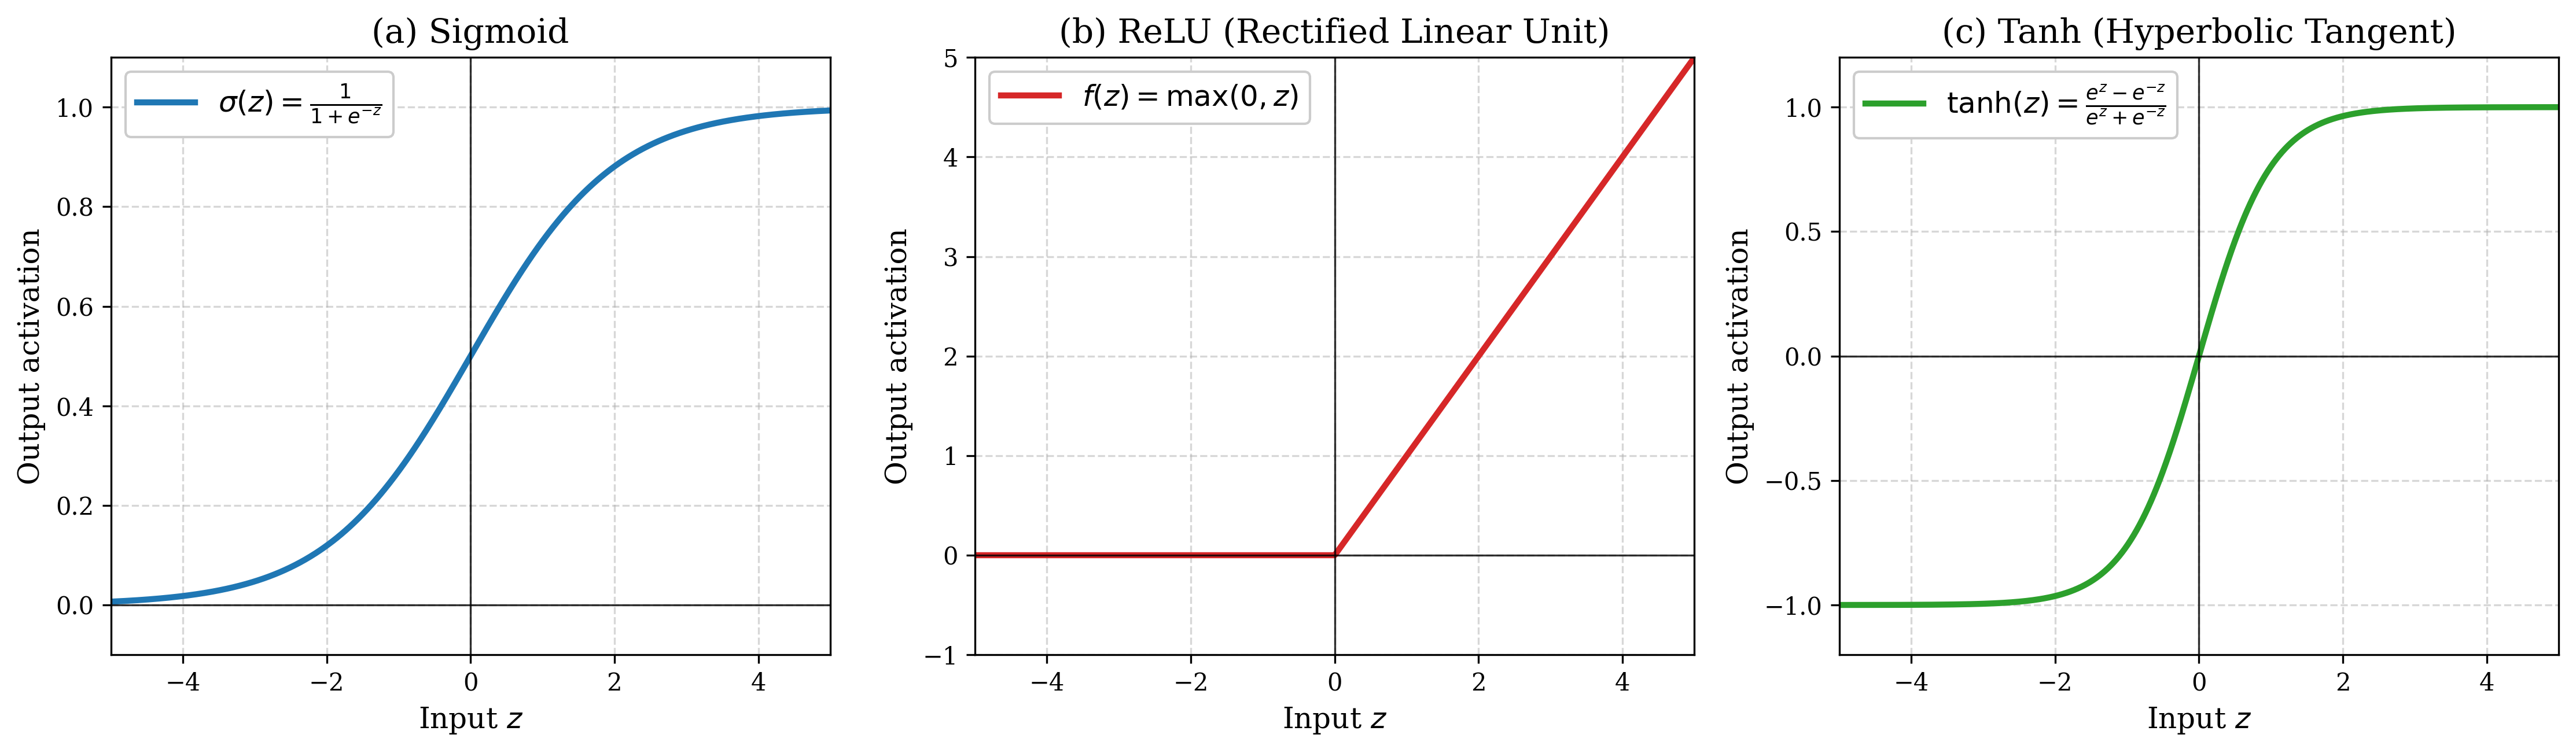
\includegraphics[width=1\textwidth]{figuras/2-fundamentos/activation_functions_combined.png}
    \caption{Activation Functions Examples: Sigmoid, ReLU, and Tanh}
    \label{fig:activation_function}
    \end{figure}

These neurons are the core components of various neural network architectures, which can be organized into layers; the input layer receives the initial data, hidden layers process the data through multiple transformations, and the output layer produces the final predictions or classifications, as shown in Figure \ref{fig:neural_network_architecture}. 
\newpage
\begin{figure}[!ht]
    \centering
    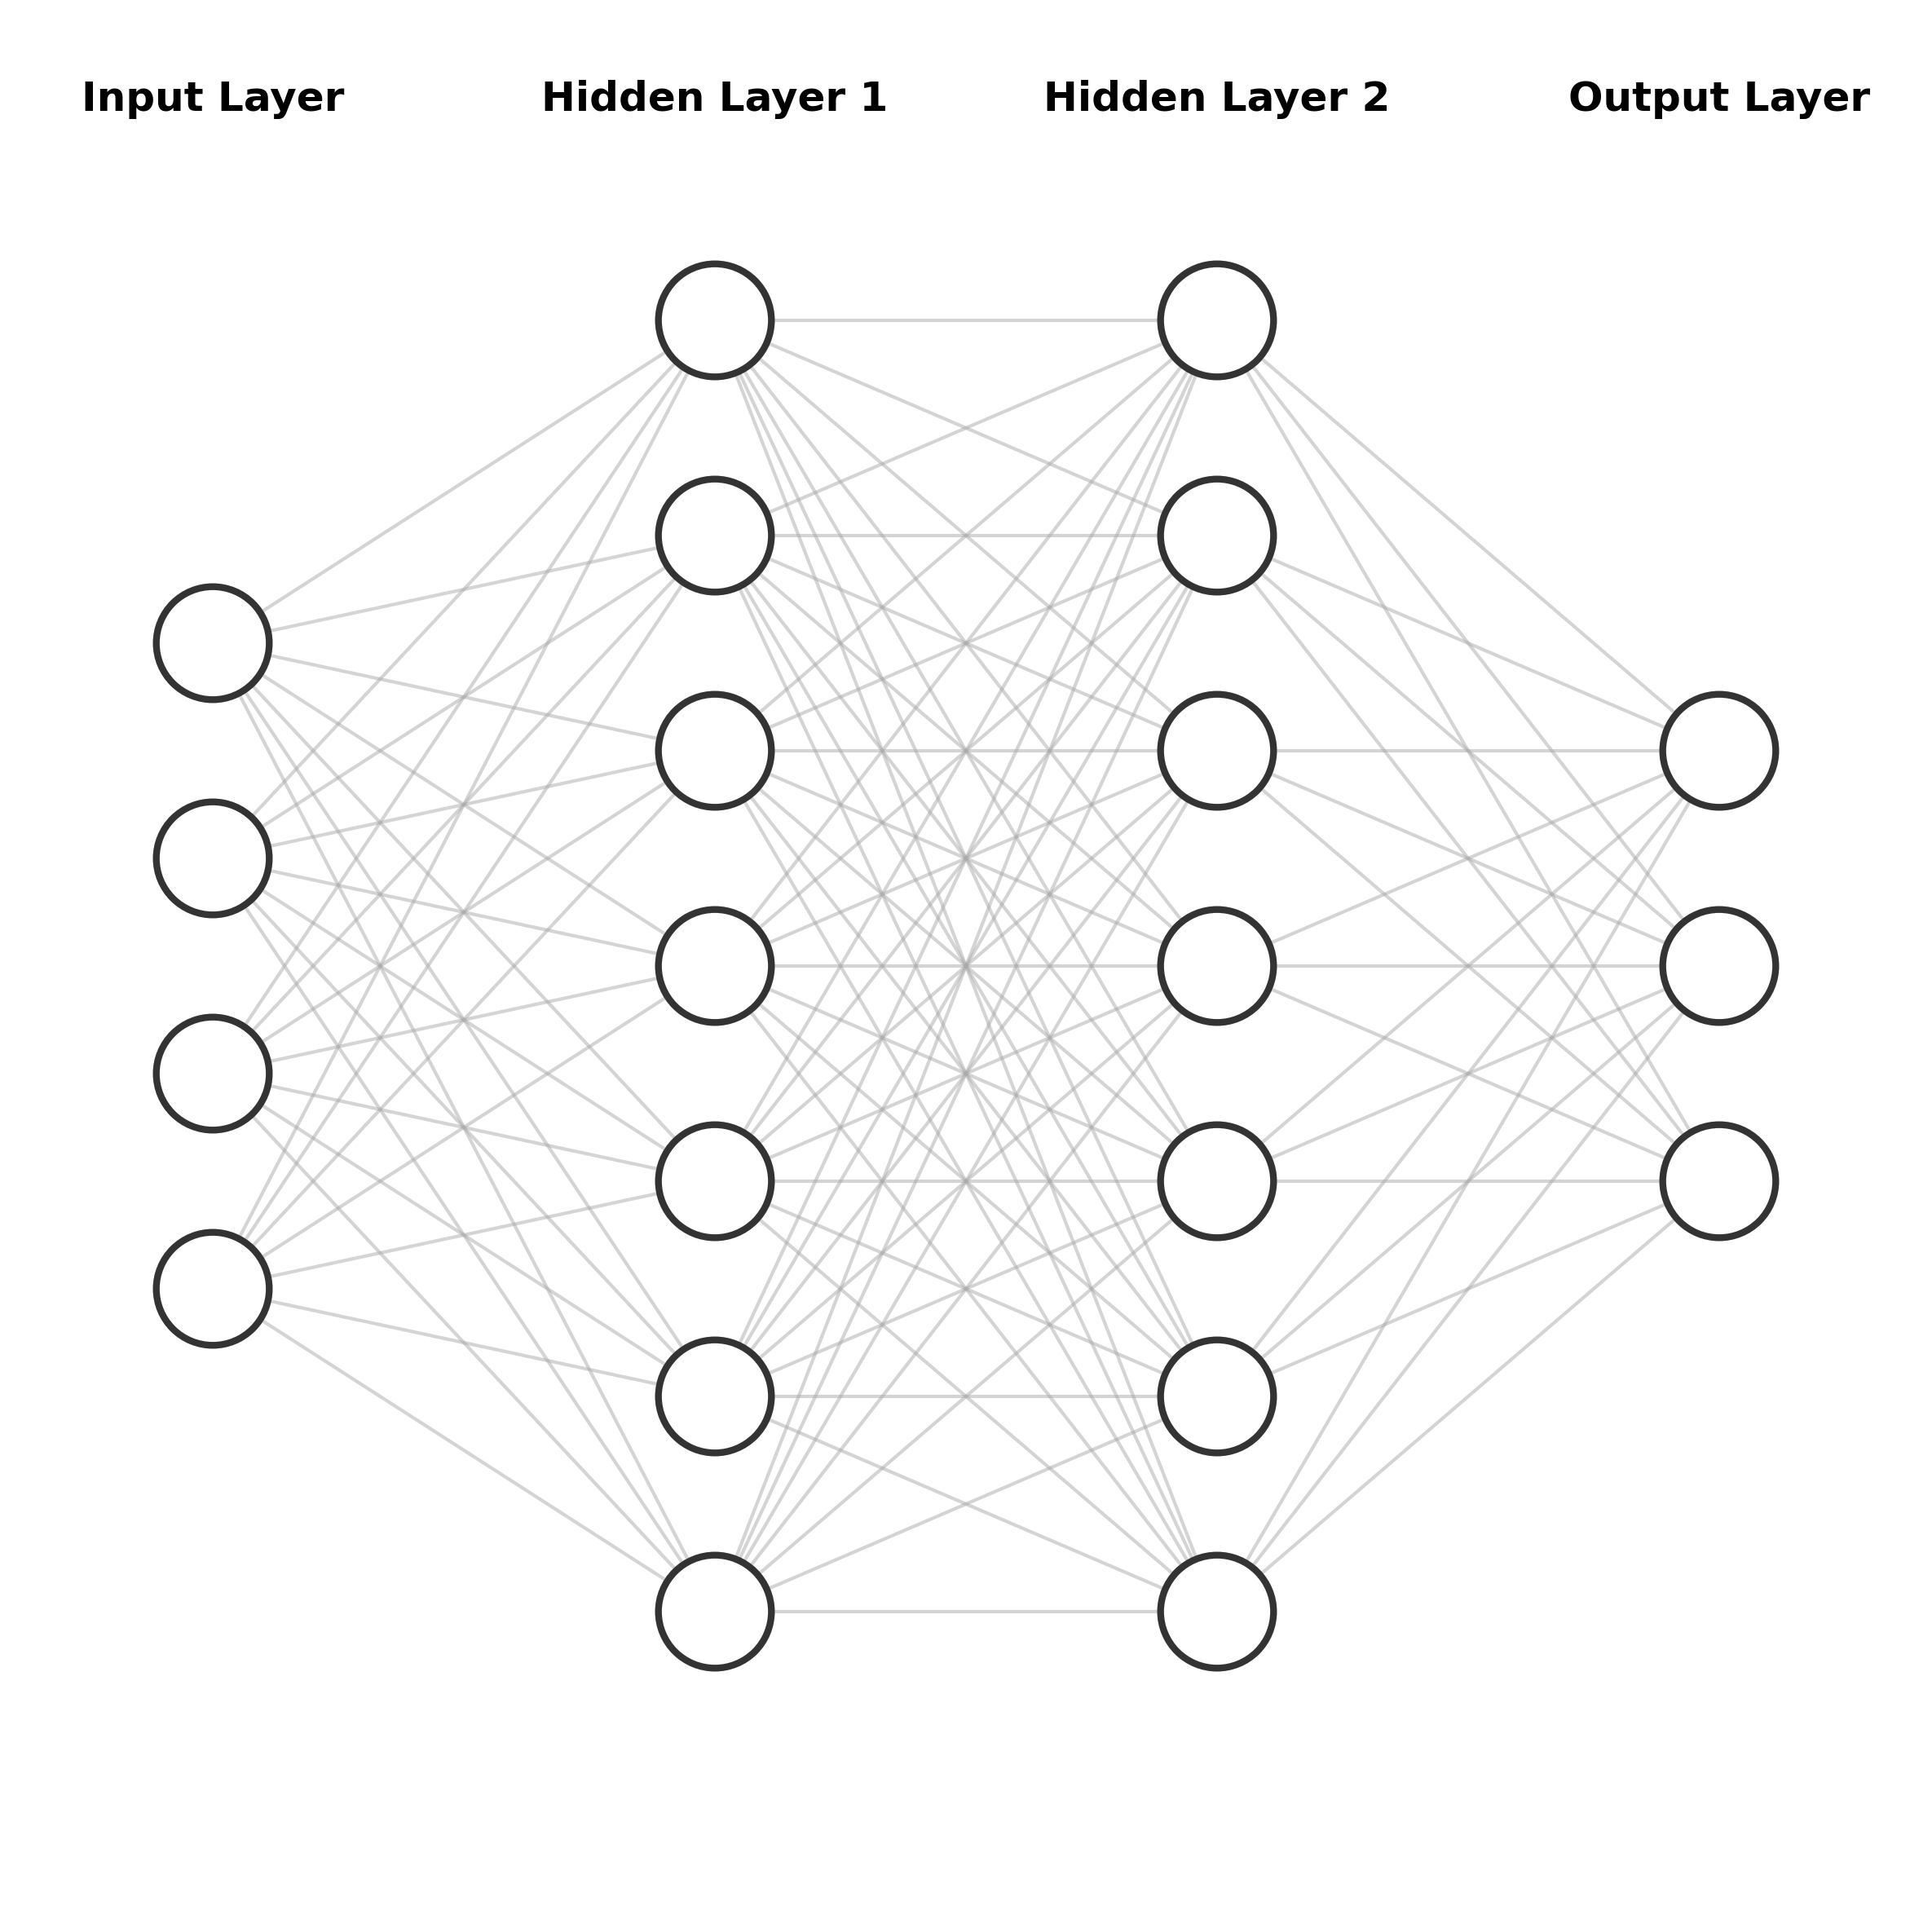
\includegraphics[width=1\textwidth]{figuras/2-fundamentos/neural_network_diagram.png}
    \caption{Diagram of a Neural Network with Input, Hidden, and Output Layers \cite{duda2001pattern}}
    \label{fig:neural_network_architecture}
    \end{figure}

  In practice, it is more convenient to express the forward computation of an entire layer using vectorized notation:
  %  \begin{align}
  %      \mathbf{z}^{[l]} &= \mathbf{W}^{[l]} \mathbf{a}^{[l-1]} + \mathbf{b}^{[l]}, \\
  %      \mathbf{a}^{[l]} &= \sigma^{[l]}\left( \mathbf{z}^{[l]} \right),
  %      \end{align}
\begin{align}
\mathbf{z}^{[l]} = \mathbf{W}^{[l]} \mathbf{a}^{[l-1]} + \mathbf{b}^{[l]}\\
\mathbf{a}^{[l]} = \mathbf{\sigma}^{[l]}(\mathbf{z}^{[l]})
\end{align}

\noindent where $\mathbf{a}^{[0]} = \mathbf{x}$ denotes the input vector, $\mathbf{W}^{[l]} \in \mathbb{R}^{n_l \times n_{l-1}}$ is the weight matrix, $\mathbf{b}^{[l]} \in \mathbb{R}^{n_l}$ is the bias vector, and $\sigma^{[l]}(\cdot)$ is the activation function applied element-wise.
\begin{comment}
    
\begin{figure}[H]
    \centering
    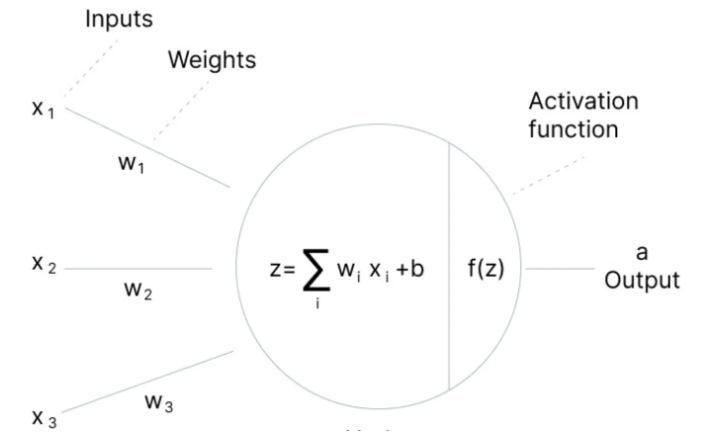
\includegraphics[width=0.8\textwidth]{figuras/2-fundamentos/neural_node.png}
    \caption{Schematic of an artificial neuron: inputs $x_i$ are weighted by $w_i$, summed with a bias $b$, and passed through a non-linear activation function $f(\cdot)$ to produce the output $y$.}
    \label{fig:neuron_diagram}
\end{figure}
\end{comment}

For supervised learning tasks, the output of the final layer $\mathbf{a}^{[L]}$ is compared with the target $\mathbf{y}$ via a differentiable loss function $\mathcal{L}(\mathbf{a}^{[L]}, \mathbf{y})$. The objective of training is to minimize the cost function:
\begin{equation}
    %J(\mathbf{W}, \mathbf{b}) = \frac{1}{m} \sum_{i=1}^m \mathcal{L}\big( \mathbf{a}^{[L](i)}, \mathbf{y}^{(i)} \big),
J(\mathbf{W}, \mathbf{b}) = \frac{1}{m} \sum_{i=1}^{m} \mathcal{L}(\mathbf{a}^{[L](i)}, \mathbf{y}^{(i)})
\end{equation}
\noindent where $m$ is the number of training samples. This minimization requires computing the gradients of $J$ with respect to each parameter $\mathbf{W}^{[l]}$ and $\mathbf{b}^{[l]}$. 

Computing these gradients is expensive due to the network's layered structure. The breakthrough of the backpropagation algorithm \cite{rumelhart1986learning} was to systematically exploit the chain rule of calculus, allowing gradients to be propagated efficiently from the output layer back through the hidden layers. This efficiency reduced the computational cost to a scale proportional to that of the forward pass, making it feasible to train networks with many layers and large numbers of parameters.

Today, neural networks form the foundation of deep learning systems used in various domains such as computer vision \cite{lecun1998gradient}, natural language processing \cite{vaswani2017attention}, and embedded AI for robotics and IoT \cite{lane2017squeezing}. Their adaptability across architectures, from convolutional neural networks (CNNs) to transformers, underscores the enduring relevance of the concepts introduced more than four decades ago.
%\textcolor{red}{this sentence uses the same style of ChatGPT :-) Please check if your text does not contain AI-written patterns} \textcolor{blue}{fixed}.


\begin{comment}
\subsection{Neural Network Architecture}

The architecture of a neural network is composed of layers of interconnected neurons. Each neuron receives inputs, applies a weighted sum followed by an activation function, and produces an output that is passed to the next layer of neurons. 

The basic building block of a neural network is the artificial neuron, which can be mathematically represented as follows:

\begin{equation}
    y = f\left(\sum_{i=1}^{n} w_i x_i + b\right)
    \end{equation}
    
    where \(y\) is the output, \(w_i\) are the weights, \(x_i\) are the inputs, \(b\) is the bias, and \(f\) is the activation function. The activation function introduces non-linearity into the model, allowing it to learn complex relationships in the data.
    
    Or visually as shown in Figure \ref{fig:neuron_diagram}, where the inputs are multiplied by their corresponding weights, summed up, and then passed through an activation function to produce the output.
    
    \newpage
    
    \begin{figure}
    \centering
    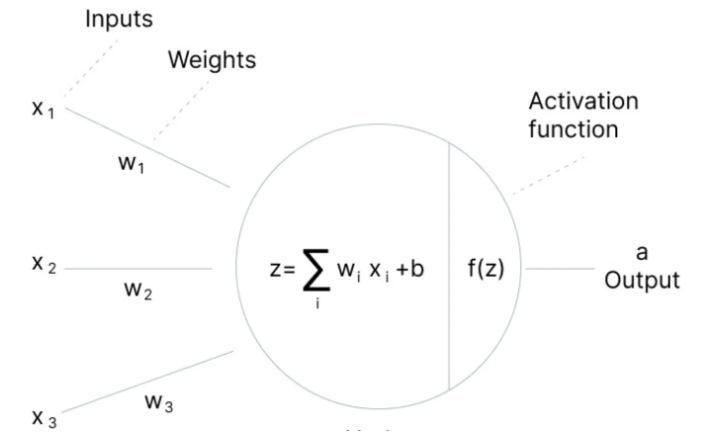
\includegraphics[width=0.8\textwidth]{figuras/2-fundamentos/neural_node.png}
    \caption{Diagram of a Single Neuron \cite{neural_node_pic}}
    
    \label{fig:neuron_diagram}
    \end{figure}
    
    Neural networks can be organized into various topologies, with the most common being Feedforward Neural Networks (FNN) and Multi-Layer Perceptrons (MLP)\cite{goodfellow2016deep}. FNNs consist of an input layer, one or more hidden layers, and an output layer, where information flows in one direction. MLPs are a specific type of FNN that includes multiple layers of neurons, allowing for more complex representations.
    
    Convolutional Neural Networks (CNNs) are another important architecture, particularly in computer vision tasks. They utilize convolutional layers to automatically learn spatial hierarchies of features from images, making them highly effective for image classification and object detection.
    
    
    % 3. Training Process
    % 3.1. Supervised Learning
    % Concept of labeled data

% Dataset split (training, validation, test)

% 3.2. Loss Functions
% MSE, Cross-Entropy (brief mention)

% 3.3. Optimization
% Gradient descent and variants (SGD, Adam)
\subsection{Training Process}
The training process of neural networks typically involves supervised learning, where the model learns from labeled data. The dataset is usually split into three parts: training, validation, and test sets. The training set is used to train the model, the validation set helps tune parameters, and the test set evaluates the model's performance on unseen data.

Loss functions are crucial in training, as they quantify the difference between the predicted outputs and the actual
labels. Common loss functions include Mean Squared Error (MSE) for regression tasks and Cross-Entropy for classification tasks shown respectively in Equations \ref{eq:mse} and \ref{eq:cross_entropy}. The choice of loss function depends on the specific task and the nature of the data.

\begin{equation}\label{eq:mse}
    \frac{1}{n} \sum_{i=1}^{n} (y_i - \hat{y}_i)^2
\end{equation}

\begin{equation}\label{eq:cross_entropy}
    -\sum_{i=1}^{n} y_i \log(\hat{y}_i)
\end{equation}

% 3.4. Backpropagation Algorithm
% How the backpropagation algorithm works
% Gradient calculation and weight updates
% Importance of backpropagation in training neural networks

These loss functions are used within backpropagation algorithm, which is the core of the training process.


% Backpropagation algorithm (brief overview or diagram)

% 4. Inference Process
% What happens when the model is deployed

% Importance of performance, size, and speed (hinting at quantization need)

% How a trained model maps input -> output

\subsubsection*{Backpropagation}
Backpropagation, short for \textit{backward propagation of errors}, is the fundamental algorithm for training artificial neural networks, enabling the efficient computation of gradients of a loss function with respect to the network’s parameters \cite{rumelhart1986learning}. It leverages the chain rule of calculus to propagate errors from the output layer back to earlier layers, systematically adjusting the weights and biases to minimize prediction error. The method was popularized in the mid-1980s, although its theoretical underpinnings can be traced back to earlier works in control theory and automatic differentiation \cite{werbos1974beyond}. Today, it remains the backbone of most supervised deep learning frameworks, being used in conjunction with optimizers such as stochastic gradient descent (SGD) and Adam.

The process begins with a \emph{forward pass}, in which the input vector $x \in \mathbb{R}^{n_0}$ is propagated layer by layer through the network. For a feedforward architecture with $L$ layers, each layer $l \in \{1, \dots, L\}$ computes a pre-activation vector $z^{[l]}$ and an activation vector $a^{[l]}$ according to
\begin{equation}
z^{[l]} = W^{[l]} a^{[l-1]} + b^{[l]}, \quad a^{[l]} = \sigma^{[l]}(z^{[l]}),
\end{equation}
where $W^{[l]} \in \mathbb{R}^{n_l \times n_{l-1}}$ is the weight matrix, $b^{[l]} \in \mathbb{R}^{n_l}$ is the bias vector, and $\sigma^{[l]}(\cdot)$ is a differentiable activation function such as the sigmoid, hyperbolic tangent, or ReLU. The input layer is given by $a^{[0]} = x$, and the network output is $\hat{y} = a^{[L]}$. The discrepancy between $\hat{y}$ and the target $y$ is measured by a differentiable loss function $\mathcal{L}(\hat{y}, y)$, and the cost over a batch of $m$ samples is
\begin{equation}
    J(W,b) = \frac{1}{m} \sum_{i=1}^{m} \mathcal{L}\big(a^{[L](i)}, y^{(i)}\big).
\end{equation}

Once the forward pass has produced the output, the \emph{backward pass} applies the chain rule to determine how a small change in each parameter affects the loss. At the output layer, the error signal is computed as
\begin{equation}
\delta^{[L]} = \nabla_a \mathcal{L}\big(a^{[L]}, y\big) \odot \sigma'^{[L]}\big(z^{[L]}\big),
\end{equation}
where $\odot$ denotes elementwise multiplication. For each preceding hidden layer $l = L-1, \dots, 1$, the error term is propagated backwards as
\begin{equation}
\delta^{[l]} = \big(W^{[l+1]}\big)^{T} \delta^{[l+1]} \odot \sigma'^{[l]}\big(z^{[l]}\big),
\end{equation}
effectively applying the chain rule to relate the sensitivity of the cost to parameters in earlier layers. Given these $\delta$ terms, the gradients with respect to the parameters are
\begin{align}
\frac{\partial J}{\partial W^{[l]}} &= \frac{1}{m} \delta^{[l]} \big(a^{[l-1]}\big)^{T}, \\
\frac{\partial J}{\partial b^{[l]}} &= \frac{1}{m} \sum_{i=1}^m \delta^{[l](i)}.
\end{align}
Finally, the parameters are updated via gradient descent,
\begin{align}
W^{[l]} &\gets W^{[l]} - \eta \frac{\partial J}{\partial W^{[l]}}, \\
b^{[l]} &\gets b^{[l]} - \eta \frac{\partial J}{\partial b^{[l]}},
\end{align}
where $\eta > 0$ is the learning rate.

The efficiency of backpropagation arises from its reuse of intermediate computations from the forward pass, avoiding redundant derivative calculations. In fact, its computational complexity is $\mathcal{O}(n)$ in the number of parameters, making it feasible for networks with millions of weights. This property, combined with the ability to use vectorized matrix operations, has made it the method of choice for modern GPUs and TPUs \cite{goodfellow2016deep}.

A high-level pseudocode for the algorithm is shown in Algorithm~\ref{alg:backprop}, where the vectorized formulation is used for batch processing. An illustration of the flow of information during forward and backward passes is provided in Figure~\ref{fig:backprop_flow}, which should be replaced with a network diagram showing activations $a^{[l]}$, pre-activations $z^{[l]}$, and gradients $\delta^{[l]}$.

\begin{figure}[H]
\centering
\includegraphics[width=0.85\linewidth]{figuras/2-fundamentos/backpropagation_flow.png}
\caption{Placeholder: Forward (left) and backward (right) propagation in a feedforward neural network \cite{duda2001pattern}}
\label{fig:backprop_flow}
\end{figure}

\begin{algorithm}[H]
\caption{Vectorized Backpropagation for a Fully Connected Neural Network}
\label{alg:backprop}
\begin{algorithmic}[1]
\Require Training data $\{(x^{(i)}, y^{(i)})\}_{i=1}^m$, learning rate $\eta$, number of layers $L$
\State Initialize $W^{[l]}, b^{[l]}$ for $l = 1, \dots, L$
\While{stopping criterion not met}
\State \textbf{Forward Pass:}
\State $A^{[0]} \gets X$
\For{$l = 1$ to $L$}
\State $Z^{[l]} \gets W^{[l]} A^{[l-1]} + b^{[l]}$
\State $A^{[l]} \gets \sigma^{[l]}(Z^{[l]})$
\EndFor
\State Compute cost $J$
\State \textbf{Backward Pass:}
\State $\Delta^{[L]} \gets \nabla_A \mathcal{L}(A^{[L]}, Y) \odot \sigma'^{[L]}(Z^{[L]})$
\For{$l = L-1$ down to $1$}
\State $\Delta^{[l]} \gets (W^{[l+1]})^T \Delta^{[l+1]} \odot \sigma'^{[l]}(Z^{[l]})$
\EndFor
\State \textbf{Parameter Updates:}
\For{$l = 1$ to $L$}
\State $W^{[l]} \gets W^{[l]} - \eta \frac{1}{m} \Delta^{[l]} (A^{[l-1]})^T$
\State $b^{[l]} \gets b^{[l]} - \eta \frac{1}{m} \sum_{i=1}^m \Delta^{[l](i)}$
\EndFor
\EndWhile
\end{algorithmic}
\end{algorithm}

From a theoretical standpoint, backpropagation can be interpreted as a special case of reverse-mode automatic differentiation, optimized for layered computational graphs. It assumes differentiable activation functions and loss functions, and its performance may degrade in very deep networks due to the vanishing and exploding gradient problems \cite{hochreiter1998vanishing}. Solutions such as careful weight initialization, normalization layers, and activation function design (e.g., ReLU, Leaky ReLU, GELU) have been developed to mitigate these issues.

In conclusion, backpropagation is the mathematical and computational framework that enables neural networks to learn from data by efficiently computing gradients through the chain rule. Its elegance lies in its generality: once the forward computation of a network is defined, the backward computation follows mechanically, allowing it to adapt seamlessly to a wide range of architectures, from simple perceptrons to modern transformers \cite{goodfellow2016deep}.

\end{comment}

During inference, the trained model is used to predict from input data. The performance, size, and speed of the model are critical factors in this process, especially in resource-constrained environments such as embedded systems and edge devices. The trained model maps input data to output predictions by applying the learned weights and biases through the network's layers.


% 5. Challenges and Motivations for Compression
% Overparameterization

% Memory usage

% Latency

% Deployment on microcontrollers, edge devices

\subsection{Challenges and Motivations for Compression}
Despite their effectiveness, ANNs face several challenges, especially Overparameterization, which can lead to significant increases in memory usage and inference latency \cite{han2016deep}. These challenges become particularly pronounced when deploying embedded systems models, where resources are limited. One standard solution to these challenges is quantization, which reduces model precision to enable faster inference and lower memory usage. 

\section{Quantization}

%1.1 Definition and Basic Idea
%General concept: reducing the precision of data by mapping continuous or high-precision values to a smaller set of fixed levels.

Quantization is a model compression technique that reduces the numerical precision of neural network parameters and activations, thereby lowering both memory usage and computational costs \cite{jacob2018quantization,han2016deep}. In summary, the idea is to map floating-point precision values to smaller, discrete fixed-precision ones. It’s by far one of the most widely used methods to make neural network computations less resource-intensive and has been proven effective for deploying ANN models on low-end devices, e.g., embedded hardware.

Mathematically, given a real-valued matrix of activations or weights $\mathbf{A} \in \mathbb{R}^{m \times p}$ and a target bit-width $n$, the quantization operator $Q$ can be defined as:
\begin{equation}
%Q(n, \mathbf{A}) = \text{clip}\left( \text{round}\left(\frac{\mathbf{A}}{q(\mathbf{A}, n)}\right)-Z,\ -2^{n-1},\ 2^{n-1}-1 \right),
Q(\mathbf{A}, n, \alpha, \beta) = \text{clip}\left(\left\lfloor \frac{\mathbf{A} - \alpha}{\frac{\beta - \alpha}{2^n - 1}} \right\rceil, 0, 2^n-1\right)\\
\label{eq:quantization}
\end{equation}
where $q(\mathbf{A}, n)$ is the scaling factor, $\text{round}(\cdot)$ rounds to the nearest integer, $\text{clip}(\cdot)$ restricts values to the range $[-2^{n-1}, 2^{n-1}-1]$ and $Z$ is an integer zero point.

The scaling factor $q(\mathbf{A}, n)$ partitions the dynamic range of $\mathbf{A}$ into $2^n$ equally spaced levels:
\begin{equation}
%q(\mathbf{A}, n) = \frac{\beta - \alpha}{2^n - 1},
q(\mathbf{A}, n) = \frac{\beta - \alpha}{2^n - 1},
\label{eq:scaling}
\end{equation}
where $\alpha = \min(\mathbf{A})$ and $\beta = \max(\mathbf{A})$. The dequantization step reconstructs an approximation $\hat{\mathbf{A}}$ of the original values:
\begin{equation}
\hat{\mathbf{A}} = q(\mathbf{A}, n) \cdot Q(n, \mathbf{A}).
\label{eq:dequantization}
\end{equation}

Figures~\ref{fig:quant_n1} and \ref{fig:quant_n2} illustrate uniform quantization for $n=1$ and $n=2$, respectively, showing the effect of reducing the representable precision.
\begin{figure}[!ht]
    \centering
    \begin{minipage}{0.8\textwidth}
        \centering
        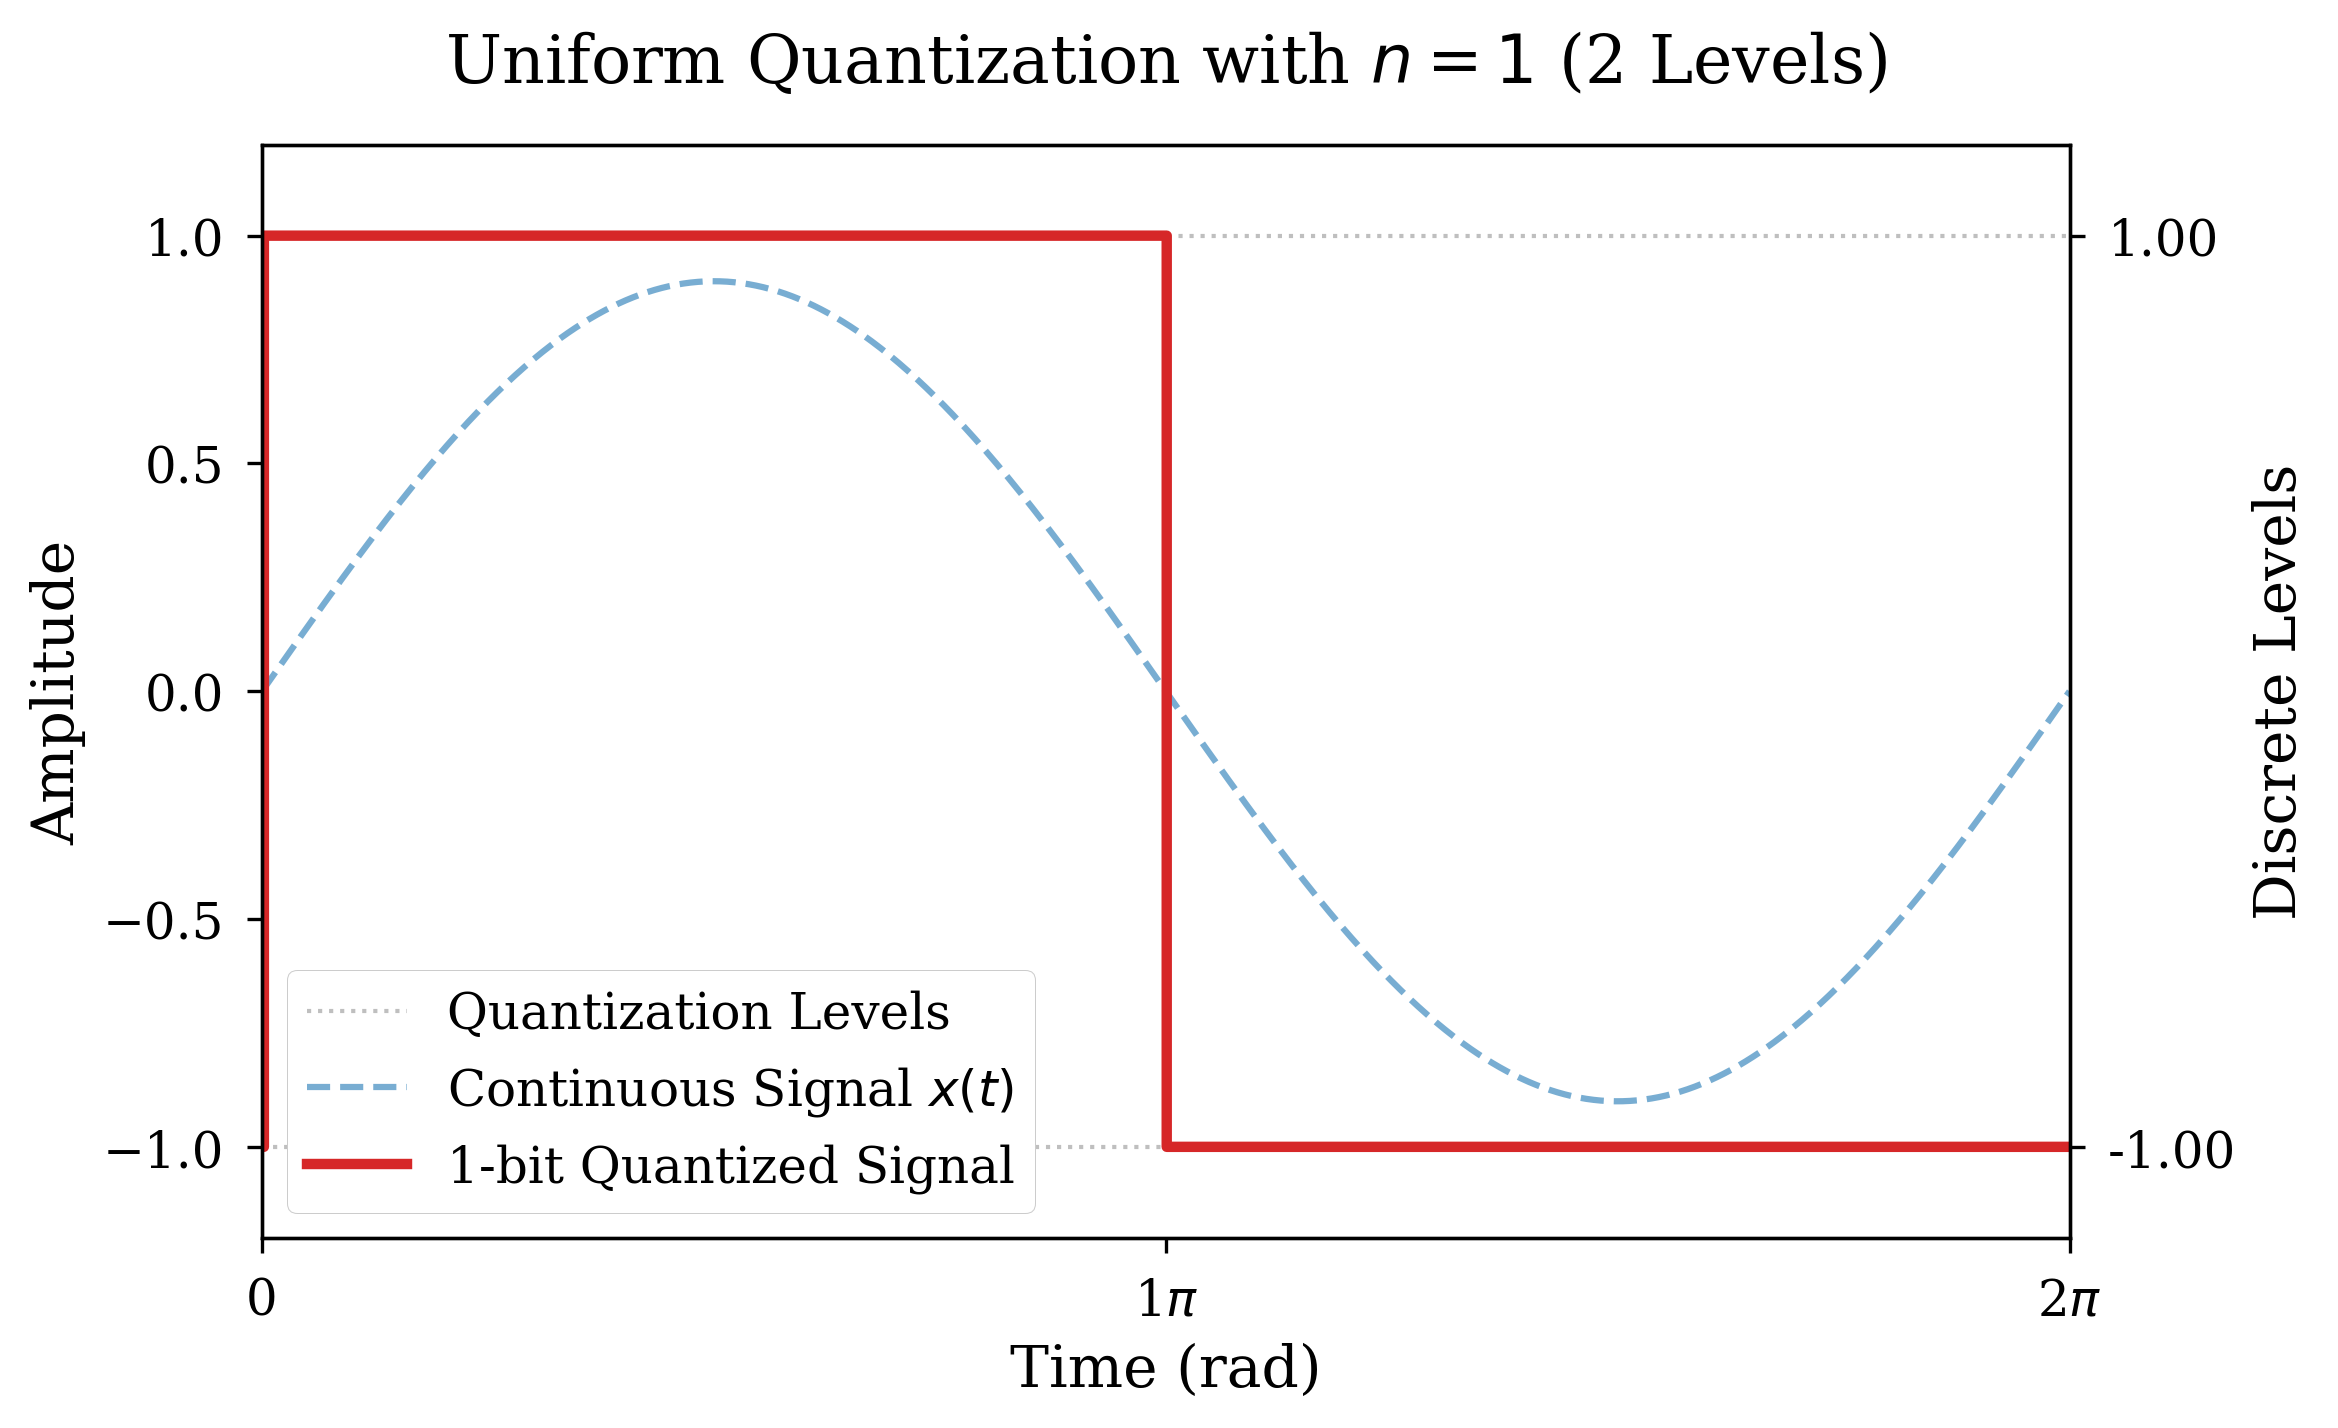
\includegraphics[width=0.75\linewidth]{figuras/2-fundamentos/quantization_n_1.png}
        \caption{Uniform quantization with $n=1$.}
        \label{fig:quant_n1}
    \end{minipage}
    \hfill
    \begin{minipage}{0.8\textwidth}
        \centering
        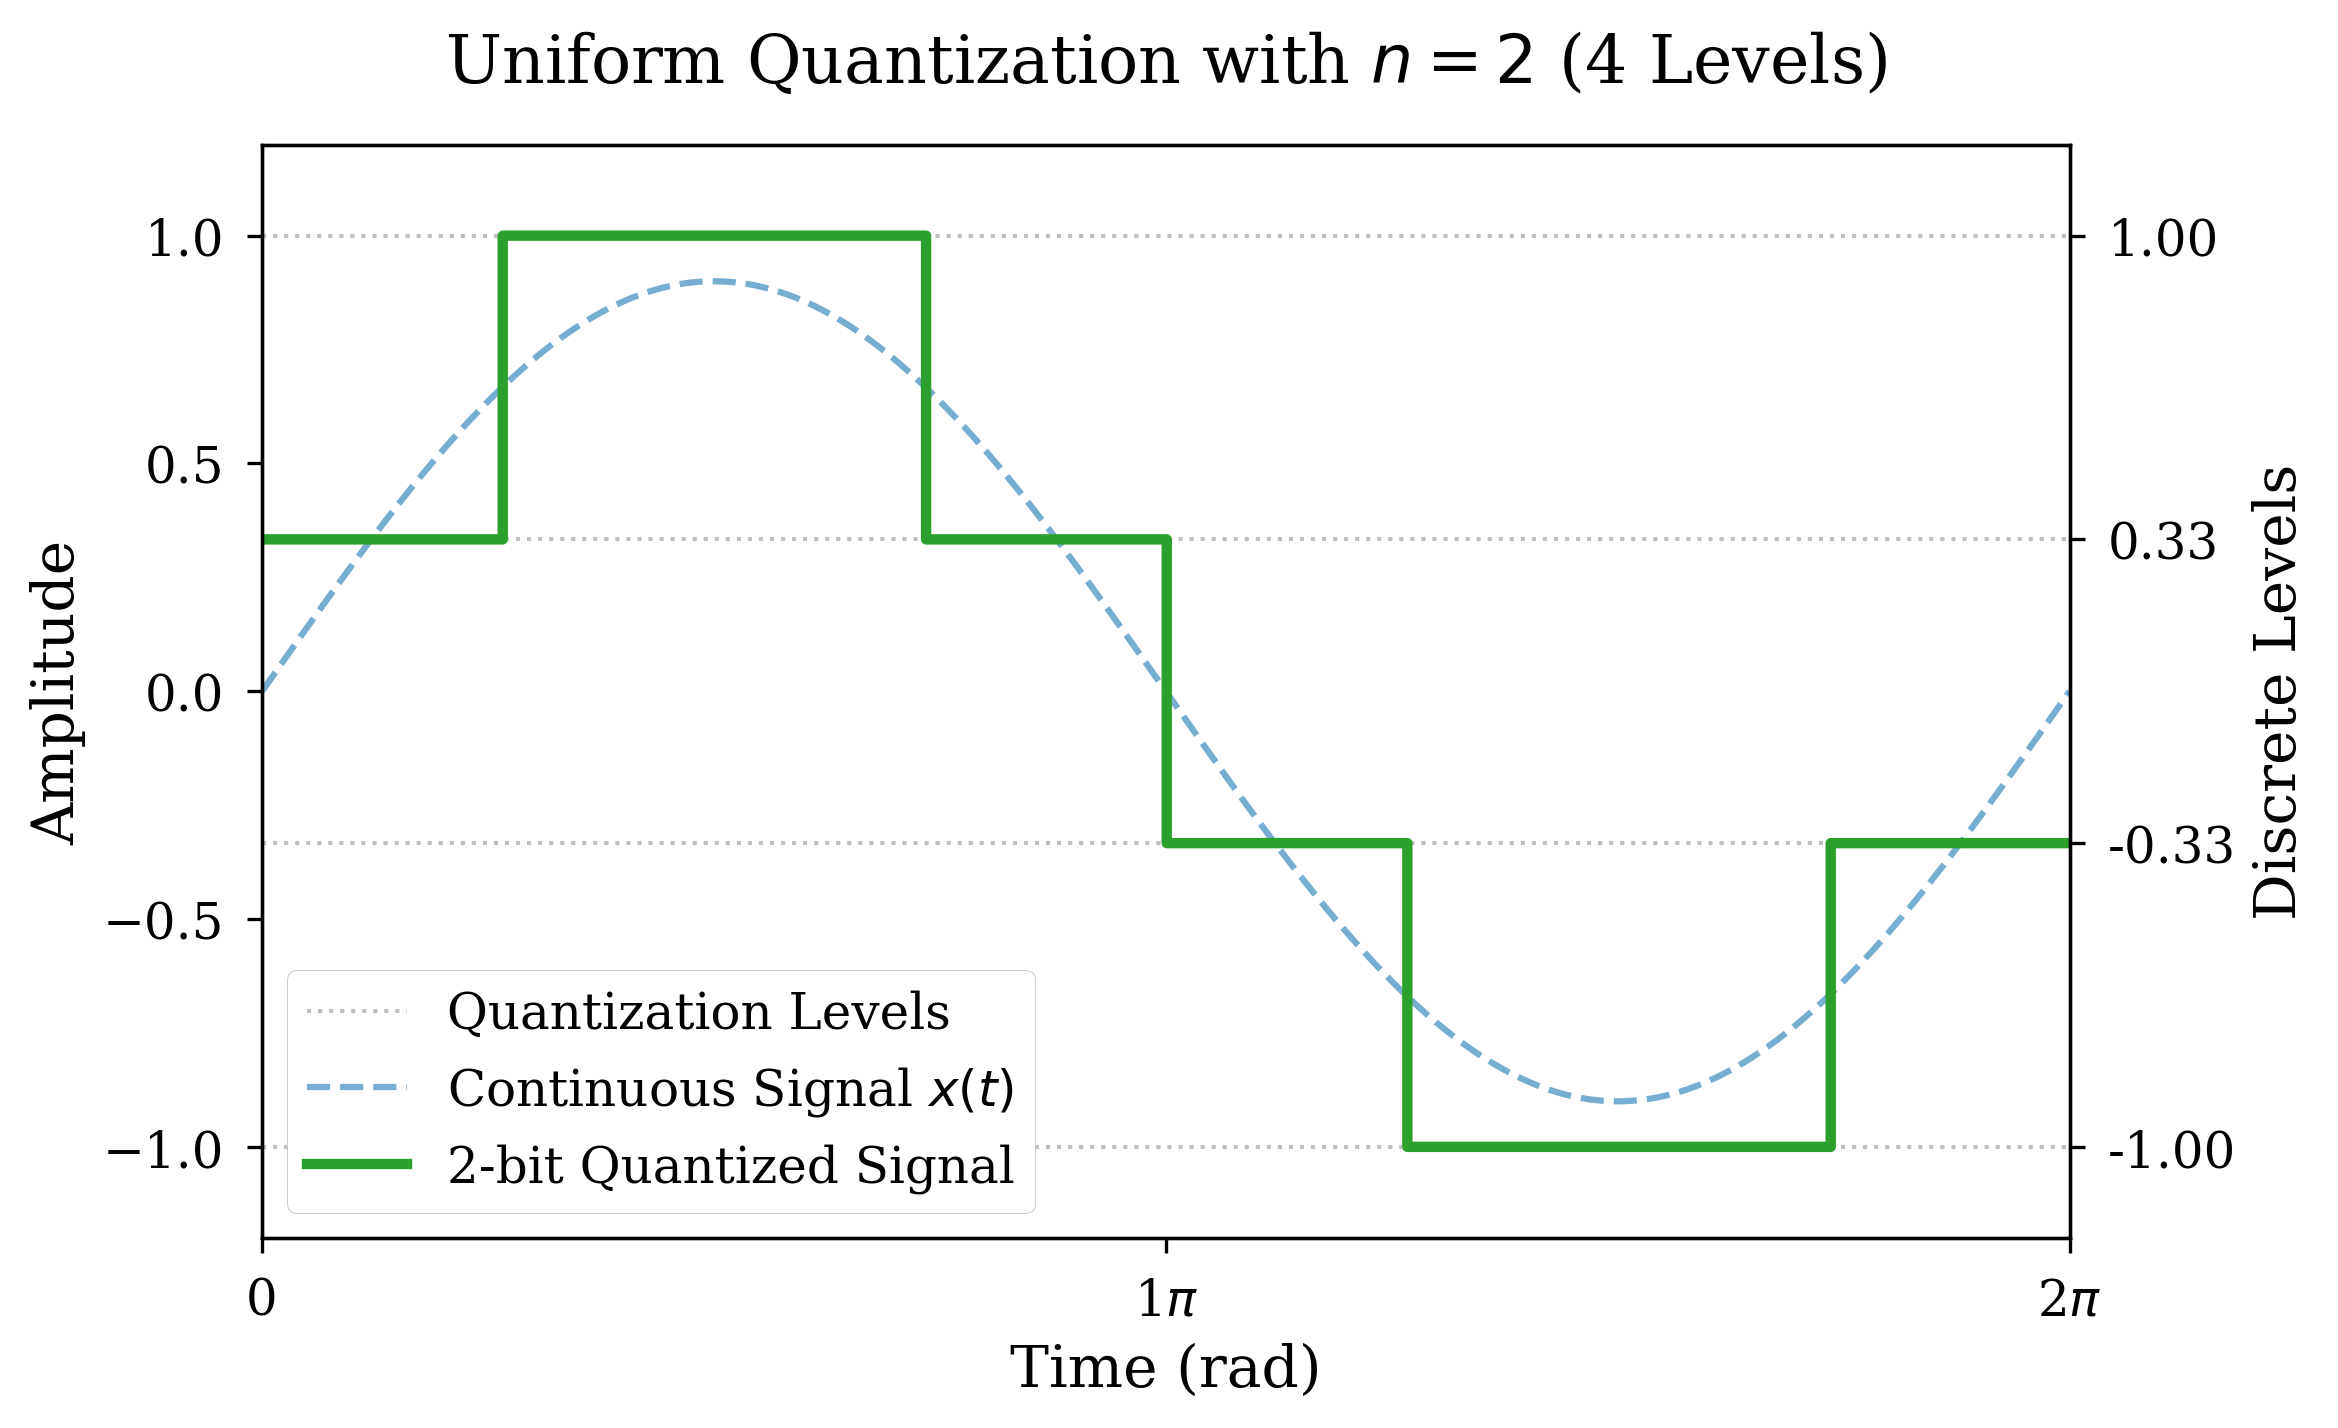
\includegraphics[width=0.75\linewidth]{figuras/2-fundamentos/quantization_n_2.png}
        \caption{Uniform quantization with $n=2$.}
        \label{fig:quant_n2}
    \end{minipage}
\end{figure}

\subsubsection*{Symmetric vs. Asymmetric Quantization}
These quantization strategies are classified as symmetric and asymmetric. In symmetric quantization, the zero-point is set to zero, and the scaling factor is applied evenly over the entire range of values, i.e., $\alpha = -\beta$. This approach is more simple and often sufficient for many applications, mainly when the distribution of values is approximately centered around zero. Consequently, symmetric quantization will be used throughout this work.

\begin{figure}[!ht]
\centering
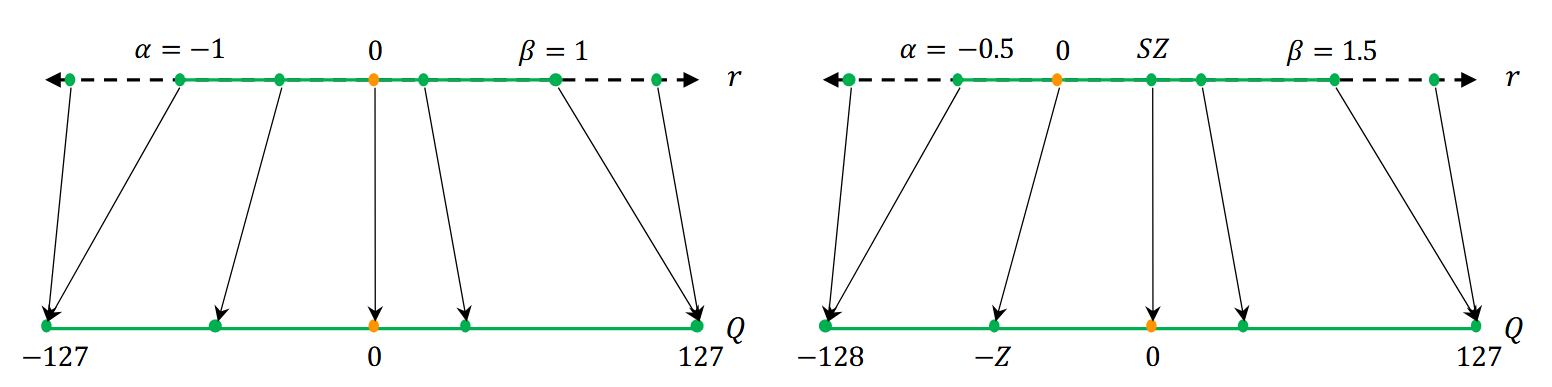
\includegraphics[width=0.8\textwidth]{figuras/2-fundamentos/quantization symetric.png}
\caption{Symmetric and asymmetric quantization.}
\label{fig:symmetric_quantization}
\end{figure}



Quantization strategies can be categorized as:
\begin{itemize}
    \item \textbf{Uniform vs. Non-uniform:} Uniform quantization uses equally spaced levels, while non-uniform uses samples from more densely populated regions.
    \item \textbf{Symmetric vs. Asymmetric:} Symmetric quantization has a zero point at zero, while asymmetric quantization allows for a non-zero zero point, which can better fit unbalanced distributions.
    %\item \textbf{Layer-wise vs. Channel-wise:} Layer-wise quantization applies a single quantization scheme to all parameters in a layer, while channel-wise quantization applies different schemes to each channel or filter, allowing for more flexibility and potentially better accuracy.
    \item \textbf{Fixed-point vs. Floating-point:} Fixed-point formats are more hardware-friendly and power-efficient, whereas low-bit floating-point formats (e.g., FP16, bfloat16) preserve a wider dynamic range.
\end{itemize}

The most crucial aspect of quantization in our scope is floating-point quantization, also called "fake quantization" \cite{gholami2021surveyquantizationmethodsefficient}, which simulates the effects of quantization during training, allowing the model to adapt and be represented in low-precision formats while maintaining the floating-point representation \cite{gholami2021surveyquantizationmethodsefficient}. Maintaining the floating-point representation \cite{gholami2021surveyquantizationmethodsefficient}. It therefore requires hardware to perform calculations in floating-point format, which is more flexible but less efficient than fixed-point arithmetic.

Fixed-point quantization represents numbers with a fixed number of bits for the integer and fractional parts, allowing for faster arithmetic operations and lower memory usage. This representation is most efficient when dealing with resource-constrained embedded devices\cite{sena2021verifying,gholami2021surveyquantizationmethodsefficient, huangEfficientVerificationQuantized2023}.

\subsection{ANN Quantization}

Strategies for quantizing ANNs are numerous, with many combinations of techniques \cite{jacob2018quantization, gholami2021surveyquantizationmethodsefficient}. The choice of strategy depends on the specific application, hardware constraints, and desired trade-offs between accuracy and efficiency. For this work, we will focus on quantizing the network’s parameters: weights, activation functions, and biases.

In general, we could use the equation \ref{eq:quantization} to quantize the weights, activations, and biases of a neural network. The quantization of the weights is performed layer by layer, where each layer $l$ has its own bit-width $n_l$:

\begin{equation}
W^{[l],q} = Q(n_l, W^{[l]}) \quad \text{for } l = 1, \dots, L,
\end{equation}
where $n_l$ is the bit-width for the $l$-th layer. The quantization of the biases follows a similar approach:
\begin{equation}
b^{[l],q} = Q(n_l, b^{[l]}) \quad \text{for } l = 1, \dots, L.
\end{equation}

However, there are considerations that must be taken into account when mapping each neural network element to the quantized representation. 

\subsubsection*{Weights}

Weights can be quantized using symmetric or asymmetric schemes \cite{gholami2021surveyquantizationmethodsefficient}. Symmetric quantization is widely adopted for weights because it simplifies the quantization function by setting the zero point ($Z$) to zero \cite{gholami2021surveyquantizationmethodsefficient}. This results in a simpler quantization function \ref{eq:quantization}, reducing computational cost during inference and making implementation more straightforward. In such cases, the clipping range is symmetric around zero, often chosen based on the maximum absolute weight. The ``full range'' approach (e.g., [-128, 127] for 8 bits) is generally more accurate than the "restricted range" (e.g., [-127, 127]) \cite{gholami2021surveyquantizationmethodsefficient}. On the other hand, asymmetric quantization uses a clipping range that is not necessarily symmetric and is preferred when weight distributions are unbalanced, as it can result in a tighter clipping range and better utilization of available bit width.

%The granularity of weight quantization is another critical factor. 
%\begin{itemize} 
%    \item Layerwise quantization applies a single clipping range to all weights within a layer. While simple to implement, it often results in sub-optimal accuracy if the range of individual convolutional filters varies widely. 
%    \item Groupwise quantization groups multiple channels within a layer to calculate the clipping range. This can be useful when parameter distributions vary significantly within a convolution but incurs an additional cost to account for different scaling factors. 
%    \item Channelwise quantization is the standard method for quantizing convolutional kernels. It assigns a dedicated scaling factor to each convolutional filter, ensuring better quantization resolution and often resulting in higher accuracy with negligible overhead. 
%    \item Sub-channelwise quantization offers the most granular control, but adds considerable overhead due to managing multiple scaling factors, making it less common. 
%\end{itemize}

Integer-only quantization, which is more desirable than simulated quantization. This is because all operations are performed using low-precision integer arithmetic \cite{gholami2021surveyquantizationmethodsefficient}, fully leveraging low-precision hardware logic that is faster, more power-efficient, and more area-efficient.

To mitigate post-quantization accuracy degradation, fine-tuning methods are employed. Quantization-Aware Training (QAT) involves retraining the model with quantized parameters to achieve lower loss and improved accuracy \cite{gholami2021surveyquantizationmethodsefficient}. QAT can also learn optimal quantization parameters, such as clipping ranges and weight scaling factors, during training. However, its main disadvantage is the high computational cost associated with extensive retraining. An alternative is Post-Training Quantization (PTQ), which quantizes and adjusts weights without retraining, offering very low, often negligible, overhead~\cite{gholami2021surveyquantizationmethodsefficient}. While faster, PTQ generally achieves lower accuracy than QAT~\cite{gholami2021surveyquantizationmethodsefficient}. For scenarios where no training/validation data is accessible, Zero-Shot Quantization (ZSQ) methods are used.

\begin{comment}
    
    Finally, to mitigate significant accuracy degradation in low-precision scenarios, mixed-precision quantization is utilized [62: \cite{gholami2021surveyquantizationmethodsefficient}; 65: \cite{gholami2021surveyquantizationmethodsefficient}]. This approach applies different bit precisions to different layers of the model [58: \cite{gholami2021surveyquantizationmethodsefficient}; 62: \cite{gholami2021surveyquantizationmethodsefficient}], with more sensitive layers kept at higher precision and less sensitive layers at lower precision [65: \cite{gholami2021surveyquantizationmethodsefficient}; 87: \cite{gholami2021surveyquantizationmethodsefficient}]. This aims to balance accuracy and efficiency across the model, minimizing accuracy degradation while still benefiting from reduced memory footprint and acceleration [65: \cite{gholami2021surveyquantizationmethodsefficient}]. Determining the optimal bit allocation per layer can involve complex search problems, such as reinforcement learning-based methods or Hessian-aware techniques [63: \cite{gholami2021surveyquantizationmethodsefficient}; 64: \cite{gholami2021surveyquantizationmethodsefficient}]. This approach has proven hardware-efficient, showing significant accelerations compared to uniform precision quantization [64: \cite{gholami2021surveyquantizationmethodsefficient}; 65: \cite{gholami2021surveyquantizationmethodsefficient}].
\end{comment}


\subsubsection*{Bias}



While the literature does not outline a single, standard quantization method for biases, there is a large discussion focused mainly on correction techniques \cite{gholami2021surveyquantizationmethodsefficient}. 

A known consequence of certain approaches, such as PTQ, is a shift in the means of the weight and activation values, which negatively impacts model accuracy. The solution lies in applying a bias correction method that seeks to readjust these deviations \cite{gholami2021surveyquantizationmethodsefficient}.

The choice between symmetric and asymmetric quantization directly influences this dynamic. In asymmetric quantization, where the clipping range is not necessarily centered at the origin, cross-terms emerge. As these terms are static, they can be absorbed by the layer's bias, thereby enabling practical hardware optimization. In contrast, symmetric quantization is inherently free of this issue, as its zero-centered range does not generate such terms.

Beyond these considerations, other techniques focus on making the neural network more amenable to quantization. Range Equalization, for example, normalizes the weight value ranges across layers, implicitly standardizing activations and lowering total error. The success of this technique is amplified in Zero-Shot Quantization scenarios, without the presence of calibration data makes bias error correction a fundamental step. Indeed, the most reliable approaches for quantization without training data often combine weight equalization and bias correction, therewith safeguarding the robustness of the quantized model.

\subsubsection*{Activations}

Quantizing activations depends on the activation function used in the ANN. For example, ReLU activations are typically quantized using symmetric quantization. Other activation functions may require asymmetric quantization. The process of quantizing activations is performed layer by layer. Each layer $l$ has its own bit-width $n_l$: 

\begin{equation}
A^{[l],q} = Q(n_l, A^{[l]}) \quad \text{for } l = 1, \dots, L,
\end{equation}

\begin{comment}
Quantizing each ANN parameter results in a loss of precision and accuracy in the quantized model due to numerical precision, known as the implementation gap between the idealized real-valued model and its finite-precision realization \cite{Cai2020Certified,cordeiro2025neuralnetworkverificationprogramming}. As discussed earlier, there are many variations in quantization. Symmetric quantization applies the same scale to the positive and negative values, while asymmetric quantization uses different scales or offsets. Uniform quantization assigns equal intervals between quantized values, whereas non-uniform quantization uses variable intervals \cite{gholami2021surveyquantizationmethodsefficient,gholami2021surveyquantizationmethodsefficient}. The number of bits used to quantize elements, as well as other techniques, also varies\cite{huangEfficientVerificationQuantized2023}. Each technique brings about a disturbance to the overall model. Considering this, safety properties were created for verification and to guide the selection of the best quantization approach for specific models.
    
\section{Vulnerabilities Introduced by Quantization}

Neural Networks have started to be used to replace work classifications that used to be done by human professionals, e.g., partten recognition professions like doctors. A computer, unlike a human, can deal with huge amounts of images and classify them as correctly as it should. However, due to new techniques of adversarial attack, the use of machine learning has become more 


Even small errors may lead to misclassification of the Neural Network due to the "error amplification effect," in which small residual adversarial noise is progressively amplified through the network's layers \cite{liaoDefenseAdversarialAttacks2018}.  

Quantization amplifies the pertubation, i.e., it makes the model more sensive to input pertubation \cite{zhangQEBVerifQuantizationError2023}, thus making the new model to misclassify more than the baseline one. It inherenly brings the model more successiable to adversarial attacks.

As explained by Sena et al. in \cite{sena2021verifying} because of less bit-width, any small pertubation may make significative changes on the hidden layers and then make the model to wronglly classify.

The quantization impacts on the decision borders \cite{gorslineAdversarialRobustnessQuantized2021}. During weight reduction, the netwroks loses the capability to define smooth borders and thus to have a precise inference between classes. This influences direcetly on gradient attacks, beacuse the attacker aims to hit the region where the missclassification happens \cite{gorslineAdversarialRobustnessQuantized2021}.

A concept defined by Giacobbe et al. in \cite{giacobbe2020how} proves that robustness is not non-monotonic bitwise, i.e., a 32 bit may become vulnerable if quantized to a 8 bit precision, but other model might as well become vulnerable if the precision is increased, e.g., from 6 to 8 for example. This phenomenon justifies the need to exist a bit-precision verification because anything can happen to a model by swapping the bit precision.

As discussed previously, Quantization introduces statistical errors into the Quantized model. These errors may affect the model's ability to classify and operate properly on input data. Thus, there is a need to assess safety features.
    My work relies on
ANNs and QNNs are like black boxes: in practice, we only control the input and observe the output, while the internal reasoning is not explicitly accessible. As a result, most safety and security properties naturally express as constraints on their input-output relations. Let $f$ be the network function mapping an input $x \in \mathcal{I}$ to an output space $\mathcal{O}$. Then, a generic safety requirement can be stated as: for every input $x \in \mathcal{I}$, the produced output must lie in a desired set $\mathcal{G}$, i.e., it must satisfy the property $P$:
\[
\forall x \in \mathcal{I} \;\Rightarrow\; f(x) \in \mathcal{G}.
\]

One important safety-related property is adversarial robustness. This property is usually regarded as the requirement that small perturbations in the input should not change the model decision. The predicted label must stay the same even if the input is slightly modified \cite{huangSurveySafetyTrustworthiness2020, linIntegerarithmeticonlyCertifiedRobustness2021}. Consider an input domain $\mathcal{D}$ and a neighborhood around a specific input $x \in \mathcal{D}$, defined by a metric $d_{\text{in}}$ and referred to as $\mathcal{I}(x,d_{\text{in}})$. If $y$ represents the correct label for $x$, robustness can be formalized as
\[
\forall  x' \in \mathcal{I}(x,d_{\text{in}}) \;\Rightarrow\; f(x') = y,
\] 

Here, $\mathcal{I}(x,d_{\text{in}})$ is typically constrained by a radius $\epsilon$. This means the distance between two values must be less than or equal to $\epsilon$, for example, $d_{\text{in}}(x,x') \le \epsilon$ \cite{huangSurveySafetyTrustworthiness2020}. This research uses an $L_\infty$ ball, which restricts the maximum deviation for each feature:
\[
\mathcal{I}(x,\epsilon) = \left\{ x' \in \mathbb{R}^n \;\middle|\; \|x - x'\|_\infty \le \epsilon \right\}.
\]
As defined in the survey \cite{huangSurveySafetyTrustworthiness2020} the adversarial attack can be defined as in Definition \ref{definition:adversarial_atttack}.
\begin{definition}[Adversarial Example]\label{definition:adversarial_atttack}
Given a ANN $f : \mathcal{I} \to \mathcal{O}$, a human decision oracle $\mathcal{H} : \mathcal I \to \mathcal{O}$, and a legitimate input $x \in \mathcal{I}$ with $\arg \max_j f_j(x) = \arg \max_j \mathcal{H}_j(x)$, an adversarial example to a ANN is defined as:
\begin{equation}
\begin{aligned}
\exists \hat{x} : \quad & \arg \max_j \mathcal{H}_j(\hat{x}) = \arg \max_j \mathcal{H}_j(x) \\
& \wedge ||x - \hat{x}||_p \leq d \\
& \wedge \arg \max_j f_j(\hat{x}) \neq \arg \max_j f_j(x)
\end{aligned}
\end{equation}
where $p \in \mathbb{N}, p \geq 1, d \in \mathbb{R}$, and $d > 0$.
\end{definition}

The cause of vulnerability to \textit{adversarial examples} is likely due to to extreme nonlinearity of Neural Network Models \cite{goodfellowExplainingHarnessingAdversarial2015}


%% New text
\subsection{Adversarial Attack Verification Using SMT}

In the context of NN, equivalence refers to the property that two neural networks can produce the same outputs given the same set of inputs. This is particularly important when considering the quantization process, which aims to reduce the network's size to fit the NN into a resource-constrained environment without significantly degrading its performance.

We define neural network equivalence in terms of their outputs over a given input space. Specifically, we consider two neural networks, $f$ and $t$, where $f$ is the original floating-point neural network and $t$ is the quantized neural network. The equivalence condition can be expressed as follows:
\begin{equation}
f(x) \sim t(x), \quad \forall x \in I,
\end{equation}
where $I$ is the input space and $O$ is the output space. This means that for every input $x$ in the input space, the output of the original neural network $f$ and the output of the quantized neural network $t$ must produce the same class label or output value.
\end{comment}

%
\section{Safety and Robustness in Quantized Neural Networks}

Neural Networks have begun to replace work previously performed by human professionals. For example, in pattern recognition, computers perform tasks similar to those of doctors. Unlike humans, a computer can process large numbers of images and classify them with high accuracy. However, new adversarial attack techniques have made the use of machine learning more challenging. Techniques such as Fast Gradient Sign Method (FGSM) \& R+FGSM \cite{goodfellowExplainingHarnessingAdversarial2015}, Random Perturbation, and Basic Interactive Method \cite{kurakin2017adversarialmachinelearningscale} allow an attacker to subtly alter the input data. These small perturbations, although imperceptible to humans, are specifically designed to cause the model to misclassify the input as defined in Definition \ref{definition:adversarial_attack} \cite{goodfellowExplainingHarnessingAdversarial2015}.
\newpage
\begin{figure}
    \centering
    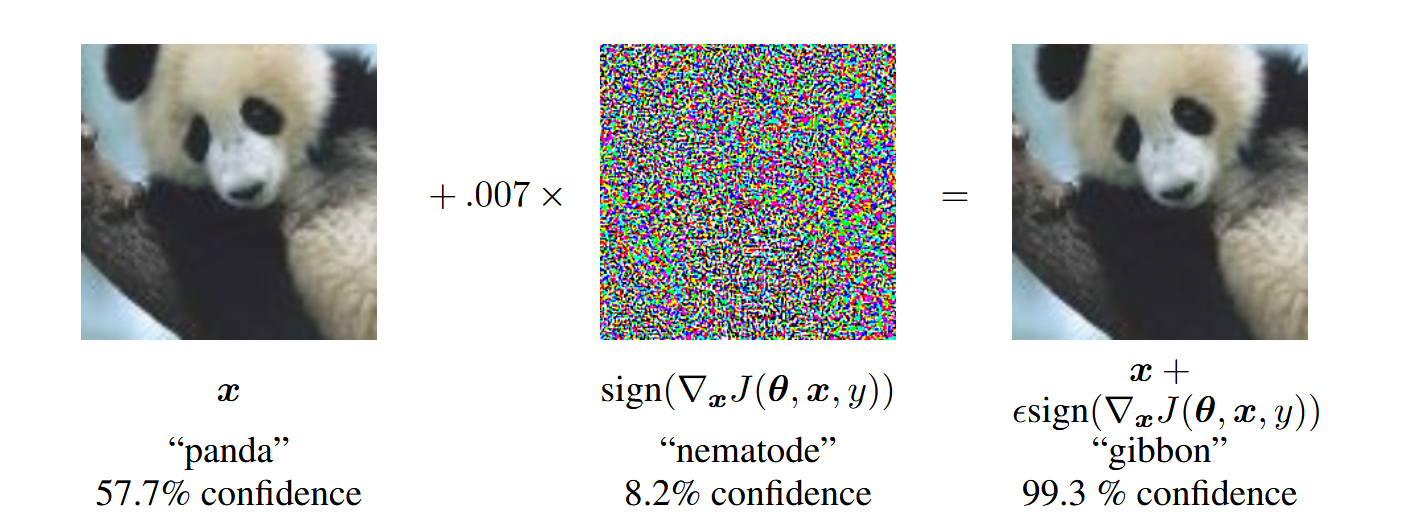
\includegraphics[width=1\textwidth]{figuras/2-fundamentos/safety/adversarial_attack_panda_example.png}
    \caption{Adversarial Attack Extracted from \cite{goodfellowExplainingHarnessingAdversarial2015}}
    \label{fig:panda_example_safety}
    \end{figure}
    
ANNs and QNNs are like black boxes: in practice, we only control the input and observe the output, while the internal reasoning is not explicitly accessible. As a result, most safety and security properties naturally express as constraints on their input-output relations. To formalize this, let $f$ be the network function mapping an input $x \in \mathcal{I}$ to an output space $\mathcal{O}$. Then, a generic safety requirement can be stated as: for every input $x \in \mathcal{I}$, the produced output must lie in a desired set $\mathcal{G}$, i.e., it must satisfy the property $P$:
\[
\forall x \in \mathcal{I} \;\Rightarrow\; f(x) \in \mathcal{G}.
\]

Building on this formal framework, one important safety-related property is adversarial robustness. This property is usually regarded as the requirement that small perturbations in the input should not change the model decision. The predicted label must stay the same even if the input is slightly modified \cite{huangSurveySafetyTrustworthiness2020, linIntegerarithmeticonlyCertifiedRobustness2021}. Consider an input domain $\mathcal{D}$ and a neighborhood around a specific input $x \in \mathcal{D}$, defined by a metric $d_{\text{in}}$ and referred to as $\mathcal{I}(x,d_{\text{in}})$. If $y$ represents the correct label for $x$, robustness can be formalized as:
\[
\forall  x' \in \mathcal{I}(x,d_{\text{in}}) \;\Rightarrow\; f(x') = y.
\] 

Here, $\mathcal{I}(x,d_{\text{in}})$ is typically constrained by a radius $\epsilon$. This means the distance between two values must be less than or equal to $\epsilon$, for example, $d_{\text{in}}(x,x') \le \epsilon$ \cite{huangSurveySafetyTrustworthiness2020}. This research uses an $L_\infty$ ball, which restricts the maximum deviation for each feature:
\[
\mathcal{I}(x,\epsilon) = \left\{ x' \in \mathbb{R}^n \;\middle|\; \|x - x'\|_\infty \le \epsilon \right\}.
\]

As defined in the survey \cite{huangSurveySafetyTrustworthiness2020}, the adversarial attack can be defined as in Definition \ref{definition:adversarial_attack}.

\begin{definition}[Adversarial Example]\label{definition:adversarial_attack}
Given an ANN $f : \mathcal{I} \to \mathcal{O}$, a human decision oracle $\mathcal{H} : \mathcal I \to \mathcal{O}$, and a legitimate input $x \in \mathcal{I}$ with $\arg \max_j f_j(x) = \arg \max_j \mathcal{H}_j(x)$, an adversarial example to an ANN is defined as:
\begin{equation}
\begin{aligned}
\exists \hat{x} : \quad & \arg \max_j \mathcal{H}_j(\hat{x}) = \arg \max_j \mathcal{H}_j(x) \\
& \wedge ||x - \hat{x}||_p \leq d \\
& \wedge \arg \max_j f_j(\hat{x}) \neq \arg \max_j f_j(x)
\end{aligned}
\end{equation}
where $p \in \mathbb{N}, p \geq 1, d \in \mathbb{R}$, and $d > 0$.
\end{definition}

The cause of vulnerability to \textit{adversarial examples} is likely due to the extreme nonlinearity of Neural Network Models \cite{goodfellowExplainingHarnessingAdversarial2015}. Even small errors may lead to misclassification of the Neural Network due to the "error amplification effect," in which small residual adversarial noise is progressively amplified through the network's layers \cite{liaoDefenseAdversarialAttacks2018}.  

\subsection*{Quantization and Robustness}
As discussed previously, Quantization introduces statistical errors into the Quantized model. These errors may affect the model's ability to classify and operate properly on input data. Thus, there is a need to assess safety features. Quantization amplifies the perturbation, i.e., it makes the model more sensitive to input perturbations \cite{zhangQEBVerifQuantizationError2023}, thereby leading the new model to misclassify more frequently than the baseline one. It inherently makes the model more susceptible to adversarial attacks. As explained by Sena et al. in \cite{sena2021verifying}, due to lower bit-width, even small perturbations can significantly alter hidden-layer activations, leading the model to misclassify.

Additionally, quantization affects decision boundaries \cite{gorslineAdversarialRobustnessQuantized2021}. During weight reduction, the network loses the ability to define smooth boundaries and thus to perform precise class inference. This directly influences gradient-based attacks, because the attacker aims to hit the region where misclassification occurs \cite{gorslineAdversarialRobustnessQuantized2021}.

In the work of \cite{goodfellowExplainingHarnessingAdversarial2015}, it's shown that the accuracy drop happens later than the adversarial vulnerability: It states that with quantization, the accuracy of the model in the work does not drop until a 4-bit bit-width is chosen, though the drop happens with 5 bit-width when attacked by the adversarial attack, dropping by 25\% the accuracy of the model.

Further supporting the need for careful analysis, a concept defined by Giacobbe et al. in \cite{giacobbe2020how} proves that robustness is not non-monotonic bitwise, i.e., a 32-bit model may become vulnerable if quantized to 8-bit precision, but another model might as well become vulnerable if the precision is increased, e.g., from 6 to 8. This phenomenon underscores the need for bit-precision verification, as anything can happen to a model when bit precision is swapped.


\section{Safety and Robustness in Quantized Neural Networks}

Neural Networks have begun to replace work previously performed by human professionals. For example, in pattern recognition, computers perform tasks similar to those of doctors. Unlike humans, a computer can process large numbers of images and classify them with high accuracy. However, new adversarial attack techniques have made the use of machine learning more challenging. Techniques such as Fast Gradient Sign Method (FGSM) \& R+FGSM \cite{goodfellowExplainingHarnessingAdversarial2015}, Random Perturbation, and Basic Interactive Method \cite{kurakin2017adversarialmachinelearningscale} allow the attacker to subtly alter the input data. These small perturbations, although imperceptible to humans, are specifically designed to cause the model to misclassify the input as defined in Definition \ref{definition:adversarial_attack} \cite{goodfellowExplainingHarnessingAdversarial2015} and seen in Figure \ref{fig:panda_example_safety}.

\newpage
\begin{figure}[!ht]
    \centering
    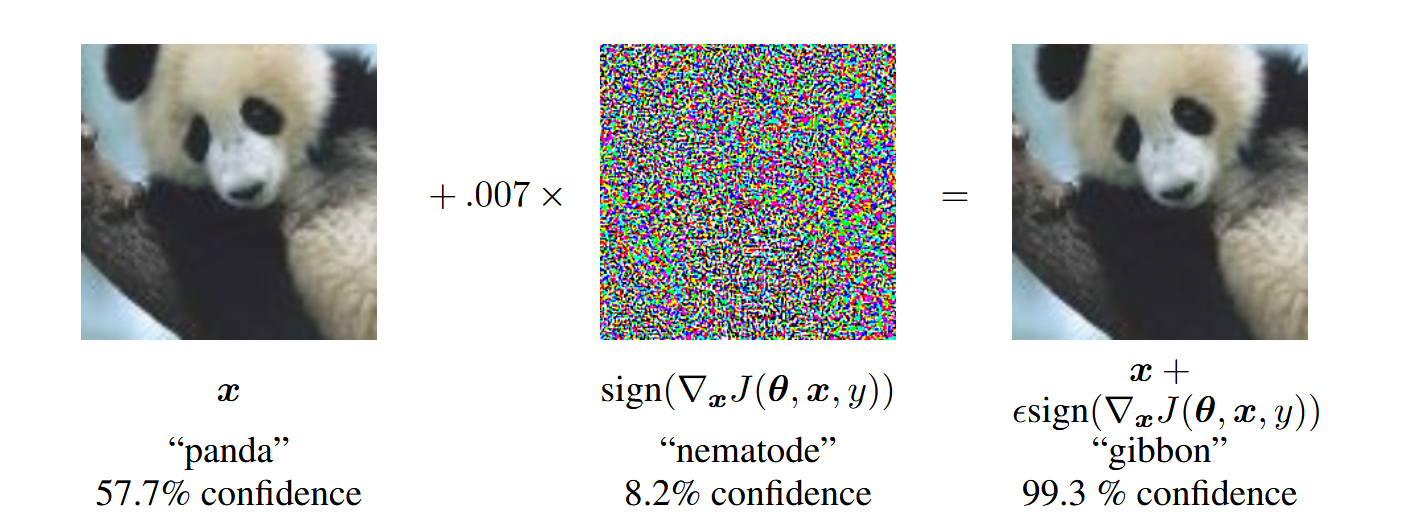
\includegraphics[width=0.8\textwidth]{figuras/2-fundamentos/safety/adversarial_attack_panda_example.png}
    \caption{Example of an adversarial Attack when a noise induces the decision maker to misclassify \cite{goodfellowExplainingHarnessingAdversarial2015}}
    \label{fig:panda_example_safety}
\end{figure}

In simpler words:
\begin{equation}
    original + perturbation = attack
\end{equation}
    
ANNs and QNNs are like black boxes: in practice, we only control the input and observe the output, while the internal reasoning is not explicitly accessible. As a result, most safety and security properties naturally express as constraints on their input-output relations. To formalize this, let $f$ be the network function mapping an input $x \in \mathcal{I}$ to an output space $\mathcal{O}$. Then, a generic safety requirement can be stated as: for every input $x \in \mathcal{I}$, the produced output must lie in a desired set $\mathcal{G}$, i.e., it must satisfy the property $\Phi$:

\begin{equation}\label{eq:security_gen_prop}
%\forall x \in \mathcal{I} \;\Rightarrow\; f(x) \in \mathcal{G}.    
 \forall \mathbf{x} \in \mathcal{I}, \quad f(\mathbf{x}) \in \mathcal{G}
 \end{equation}


It is very important to make a clear ditiguish between global and local robustness. The Equation \ref{eq:security_gen_prop} described the former by implying verification of the whole input space. However, it would lead to state explosions, as there are a infinite number of valid inputs \cite{huangSafetyVerificationDeep2017}. Consequently, formal verification often retricts is scope to a small set of training data to prove local robustness around that points. 

Building on this formal framework, one important safety-related property is local adversarial robustness. This property is usually regarded as the requirement that small perturbations in the input should not change the model decision. The predicted label must stay the same even if the input is slightly modified \cite{huangSurveySafetyTrustworthiness2020, linIntegerarithmeticonlyCertifiedRobustness2021}. Consider an input domain $\mathcal{I}$ and a neighborhood around a specific input $x \in \mathcal{I}$, defined by a metric $d_{\text{in}}$ and referred to as $\mathcal{I}(x,d_{\text{in}})$. If $y$ represents the correct label for $x$, robustness can be formalized as:
\begin{equation}\label{eq:local_robustness}
 \forall \, \mathbf{x}' \in \mathcal{B}_\infty(\mathbf{x}, \epsilon), \quad \arg\max f(\mathbf{x}') = \arg\max f(\mathbf{x}) 
\end{equation}


Here, $\mathcal{B}(x,\epsilon)$ is typically constrained by a radius $\epsilon$. This means the distance between two values must be less than or equal to $\epsilon$, for example, $d_{\text{in}}(x,x') \le \epsilon$ \cite{huangSurveySafetyTrustworthiness2020}. This research uses an $\ell_\infty$ ball, which restricts the maximum deviation for each feature:
\[
 \text{where } \mathcal{B}_{\infty}(\mathbf{x}, \epsilon) = \{\mathbf{x}' : \|\mathbf{x}' - \mathbf{x}\|_\infty \leq \epsilon\}
\] 

As defined in the survey \cite{huangSurveySafetyTrustworthiness2020}, the adversarial attack can be defined as in Definition \ref{definition:adversarial_attack}.

\begin{definition}[Adversarial Example]\label{definition:adversarial_attack}
Given an ANN $f : \mathcal{I} \to \mathcal{O}$, a human decision oracle $\mathcal{H} : \mathcal I \to \mathcal{O}$, and a legitimate input $x \in \mathcal{I}$ with $\arg \max_j f_j(x) = \arg \max_j \mathcal{H}_j(x)$, an adversarial example to an ANN is defined as:
\begin{equation}
\begin{aligned}
\exists \, \hat{x} : \quad & \arg \max_j \mathcal{H}_j(\hat{x}) = \arg \max_j \mathcal{H}_j(x) \\
& \wedge ||x - \hat{x}||_{\infty} \leq d_{in} \\
& \wedge \arg \max_j f_j(\hat{x}) \neq \arg \max_j f_j(x)
\end{aligned}
\end{equation}
\end{definition}

\textcolor{blue}{The equation above will be replaced by the below}


The cause of vulnerability to \textit{adversarial examples} is likely due to the extreme nonlinearity of Neural Network Models \cite{goodfellowExplainingHarnessingAdversarial2015}. Even small errors may lead to misclassification of the Neural Network due to the "error amplification effect," in which small residual adversarial noise is progressively amplified through the network's layers \cite{liaoDefenseAdversarialAttacks2018}.  

\subsection*{Quantization and Robustness Against Adversarial Attack}
As discussed previously, Quantization introduces statistical errors into the Quantized model. These errors may affect the model's ability to classify and operate properly on input data. Thus, there is a need to assess safety features. Quantization amplifies the perturbation, i.e., it makes the model more sensitive to input perturbations \cite{zhangQEBVerifQuantizationError2023}, thereby leading the new model to misclassify more frequently than the baseline one. It inherently makes the model more susceptible to adversarial attacks. As explained by Sena et al. in \cite{sena2021verifying}, due to lower bit-width, even small perturbations can significantly alter hidden-layer activations, leading the model to misclassify.

Additionally, quantization affects decision boundaries \cite{gorslineAdversarialRobustnessQuantized2021}. During weight reduction, the network loses the ability to define smooth boundaries and thus to perform precise class inference. This directly influences gradient-based attacks, because the attacker aims to hit the region where misclassification occurs \cite{gorslineAdversarialRobustnessQuantized2021}.

%In the work of Goodfellow et al. \cite{goodfellowExplainingHarnessingAdversarial2015}, it's shown that the accuracy drop happens later than the adversarial vulnerability: It states that with quantization, the accuracy of the model in the work does not drop until a 4-bit bit-width is chosen, though the drop happens with 5 bit-width when attacked by the adversarial attack, dropping by 25\% the accuracy of the model.
The experiments conducted by Goodfellow et al. \cite{goodfellowExplainingHarnessingAdversarial2015} show that, in Quantized models, the accuracy on the training dataset remains almost unchanged until 4-bit quantization is used. However, unlike the previous result, once an adversarial attack is induced, the accuracy drop occurs much earlier at 5 bit-width, dropping by 25\%. It shows that the model, once quantized, will not suffer from accuracy loss but will become much more vulnerable to adversarial attacks.

Further supporting the need for careful analysis, a concept defined by Giacobbe et al. in \cite{giacobbe2020how} proves that robustness is not nonmonotonic bitwise, i.e., the NN behavior after quantization is unpredictable, a 32-bit model may become vulnerable if quantized to 8-bit precision, whereas another model might as well become vulnerable if the precision is increased, e.g., from 6 to 8 bit-width. This phenomenon underscores the need for bit-precision verification, as anything can happen to a model when bit precision is swapped.

\section{Formal Verification of Quantized Neural Networks}
\begin{comment}
    
The story of Formal Verification started by Schuele and Schneider \cite{article_schule_schneider} which stabilied the based of Bound Model Checking to finite states. And though the focus wasn't to verify ANN, they introduced crucial ideas as reduct the problem of verification to a problem of logical satisfiability. These techniques is what would later allow to reduct the verification problem to an SMT problem years later.

Following this breakthrough,  Pulina et al. \cite{pulinaAbstractionRefinementApproachVerification2010} were the pioneer to use SMT verification in MLPs



To proactively prevent network vulnerabilities, a new verification area was established or revived. This development followed the findings of \cite{gorslineAdversarialRobustnessQuantized2021, kurakin2017adversarialmachinelearningscale}. These attacks intentionally mislead critical systems into incorrect classifications to achieve malicious goals. As a reprisal, several methods were developed to investigate the issue. In our line of work, we will focus on the works that use constraints to define security properties called deterministic guarantees \cite{gholami2021surveyquantizationmethodsefficient}.


\textit{Deterministic} guarantees are realized by transforming the verification problem into a set of constraints (e.g., asserts and assume statements) to be solved by a constraint solver, e.g, MILP solvers or SAT/SMT solvers. The name deterministic comes from the fact that these solvers return a deterministic answer to a query, i.e., either satisfiable or unsatisfiable \cite{gholami2021surveyquantizationmethodsefficient}.

The goal would be to use SMT solvers to verify properties like \ref{eq:security_gen_prop}.

SMT used in the literature extends to Z3, CV4, and Boolevector.

Recent works have shown that verifying Neural Networks with bit-precision is a PS-Hard task \cite{henzinger2021scalable}, thus harder than verifying floating-point Neural Networks.

Baranowski et al. developed a new background theory for fixed-point representation to be verified \cite{baranowski2020smt} that would be ideal to verify with bit-precision QNNs, as the 

SMT has been used to verify robustness from adversarial attacks 

Katz et al. introduced Reluplex to check local robustness on neural networks that use ReLu activation function, and it proves that small perturbations $\ell_\infty$ do not bring about misclassification \cite{katz2017reluplex}. Later Katz et al. and Wu et al. created a new framework called Marabou to verify adversarial robustness at large-scale neural networks. It expanded Reluplex to support any activation fuction \cite{katz2017reluplex, katz2019marabou, wuMarabou20Versatile2024}

Like our work, Huang et al. proposed verification of robustness layer-by-layer \cite{huangSafetyVerificationDeep2017}.

The first work to work with a robustness check of a Quantized Neural Network was Giacobbe, Henzinger, and Lechner at \cite{giacobbe2020how, henzinger2021scalable}. They introduced the use of bit vector theory to verify bit-precise and were the first to demonstrate that the quantization is not monotonic, thus the increase in bit precision can counter-intuitively increase the vulnerability of the model.

Amir et al. extended Marabou  to support $sign(x)$ activation function for the first time and also worked with binarized layers, which is a special case of quantization as it requires only one bit of precision.

among other works such such as \cite{song2021qnnverifier, sena2021verifying}

\subsection{SMT encoding}
In order to verify NN with bit-precision, the NN must be transformed to a code problem instead of a model problem, as it will be embarked into specific hardware, thus the first step is to transform the model into a C code \cite{cordeiro2025neuralnetworkverificationprogramming}. Once into C code, the next step is to transform the constraints into a satisfiability problem, i.e., encode the neural network layer ${f}_{n}$ into an SMT formula that will verify if by inputting a perturbation $\epsilon$ the known layer will be misclassified.
\end{comment}

%%%
The story of Formal Verification started by Schuele and Schneider \cite{article_schule_schneider}, which established the basis of Bounded Model Checking for finite states. Although their focus wasn't to verify {ANNs}, they introduced crucial ideas, such as reducing the verification problem to a problem of logical satisfiability. These techniques are what would later allow reducing the verification problem to an SMT problem years later. Following this breakthrough, Pulina et al. \cite{pulinaAbstractionRefinementApproachVerification2010} were the pioneers in using SMT verification for MLPs.

To proactively prevent network vulnerabilities, a new verification area was established or revived. This development followed the findings of \cite{gorslineAdversarialRobustnessQuantized2021, kurakin2017adversarialmachinelearningscale}, which showed that attacks can intentionally mislead critical systems into incorrect classifications to achieve malicious goals. In response, several methods were developed to investigate the issue. In our line of work, we will focus on works that use constraints to define security properties called deterministic guarantees \cite{gholami2021surveyquantizationmethodsefficient}.

{Deterministic} guarantees are realized by transforming the verification problem into a set of constraints (e.g., \texttt{assert} and \texttt{assume} statements) to be solved by a constraint solver, e.g., MILP solvers or SAT/SMT solvers. The name "deterministic" comes from the fact that these solvers return a deterministic answer to a query, i.e., either \textit{satisfiable} or \textit{unsatisfiable} \cite{gholami2021surveyquantizationmethodsefficient}. The goal is to use SMT solvers to verify properties like Equation \ref{eq:security_gen_prop}. SMT solvers used in the literature extend to Z3 , CVC4, and Boolector \cite{de2008z3, barrett2011cvc4, brummayer2009boolector} as solvable backend.

Recent works have shown that verifying Neural Networks with bit-precision is PSPACE-hard \cite{henzinger2021scalable}, making it harder than verifying floating-point Neural Networks. However, Baranowski et al. developed a new background theory for fixed-point representation \cite{baranowski2020smt} that is ideal for verifying bit-precision QNNs. This theory was integrated into off-the-shelf ESBMC, enabling QNN operations to be treated as verifiable C code \cite{song2021qnnverifier}. Through Operational Models, ESBMC faithfully captures the effects of rounding and overflow, enabling the search for adversarial counterexamples to account for the finite precision of the target hardware. Thus, the implementation in ESBMC resolves the semantic inconsistencies common to verifiers based on real representations, providing robustness guarantees that are solid for a deployment-constrained system.

SMT has been used extensively to verify robustness against adversarial attacks. Katz et al. introduced Reluplex to check local robustness on neural networks that use the ReLU activation function, proving that small perturbations $\ell_\infty$ do not bring about misclassification \cite{katz2017reluplex}. Later, Katz et al. and Wu et al. created a new framework called Marabou to verify adversarial robustness for large-scale neural networks, expanding Reluplex to support any activation function \cite{katz2017reluplex, katz2019marabou, wuMarabou20Versatile2024}. Like our work, Huang et al. proposed verification of robustness layer-by-layer \cite{huangSafetyVerificationDeep2017}.

The first work to address the robustness check of a Quantized Neural Network was by Giacobbe and Henzinger \cite{giacobbe2020how, henzinger2021scalable}. They introduced the use of bit-vector theory to verify bit-precision and were the first to demonstrate that quantization is nonmonotonic; thus, an increase in bit precision can counter-intuitively increase the vulnerability of the model. Amir et al. extended Marabou to support the $sign(x)$ activation function for the first time and also worked with binarized layers, which is a special case of quantization as it requires only one bit of precision. This field includes other works such as \cite{song2021qnnverifier, sena2021verifying}.

Instead of relying on heuristic adversarial attacks like FGSM to assess robustness, this work will use $\ell_\infty$-norm ball perturbation as it is more aligned with other formal methods in the literature \cite{cai2025certified, sena2021verifying}, as Gradient-based attacks (like PGD or JSMA) are incomplete, i.e., they can find vulnerabilities, but cannot prove their absence \cite{huangSafetyVerificationDeep2017}. It will allow our framework to verify whether, under a uniform-interval perturbation $\epsilon$, the network is safe and sound; therefore, allowing us to verify the local robustness property \ref{eq:local_robustness}. The affirmation can be visually checked in the Figure \ref{fig:uniform_norm_verification}.

\begin{figure}[!ht]
    \centering
    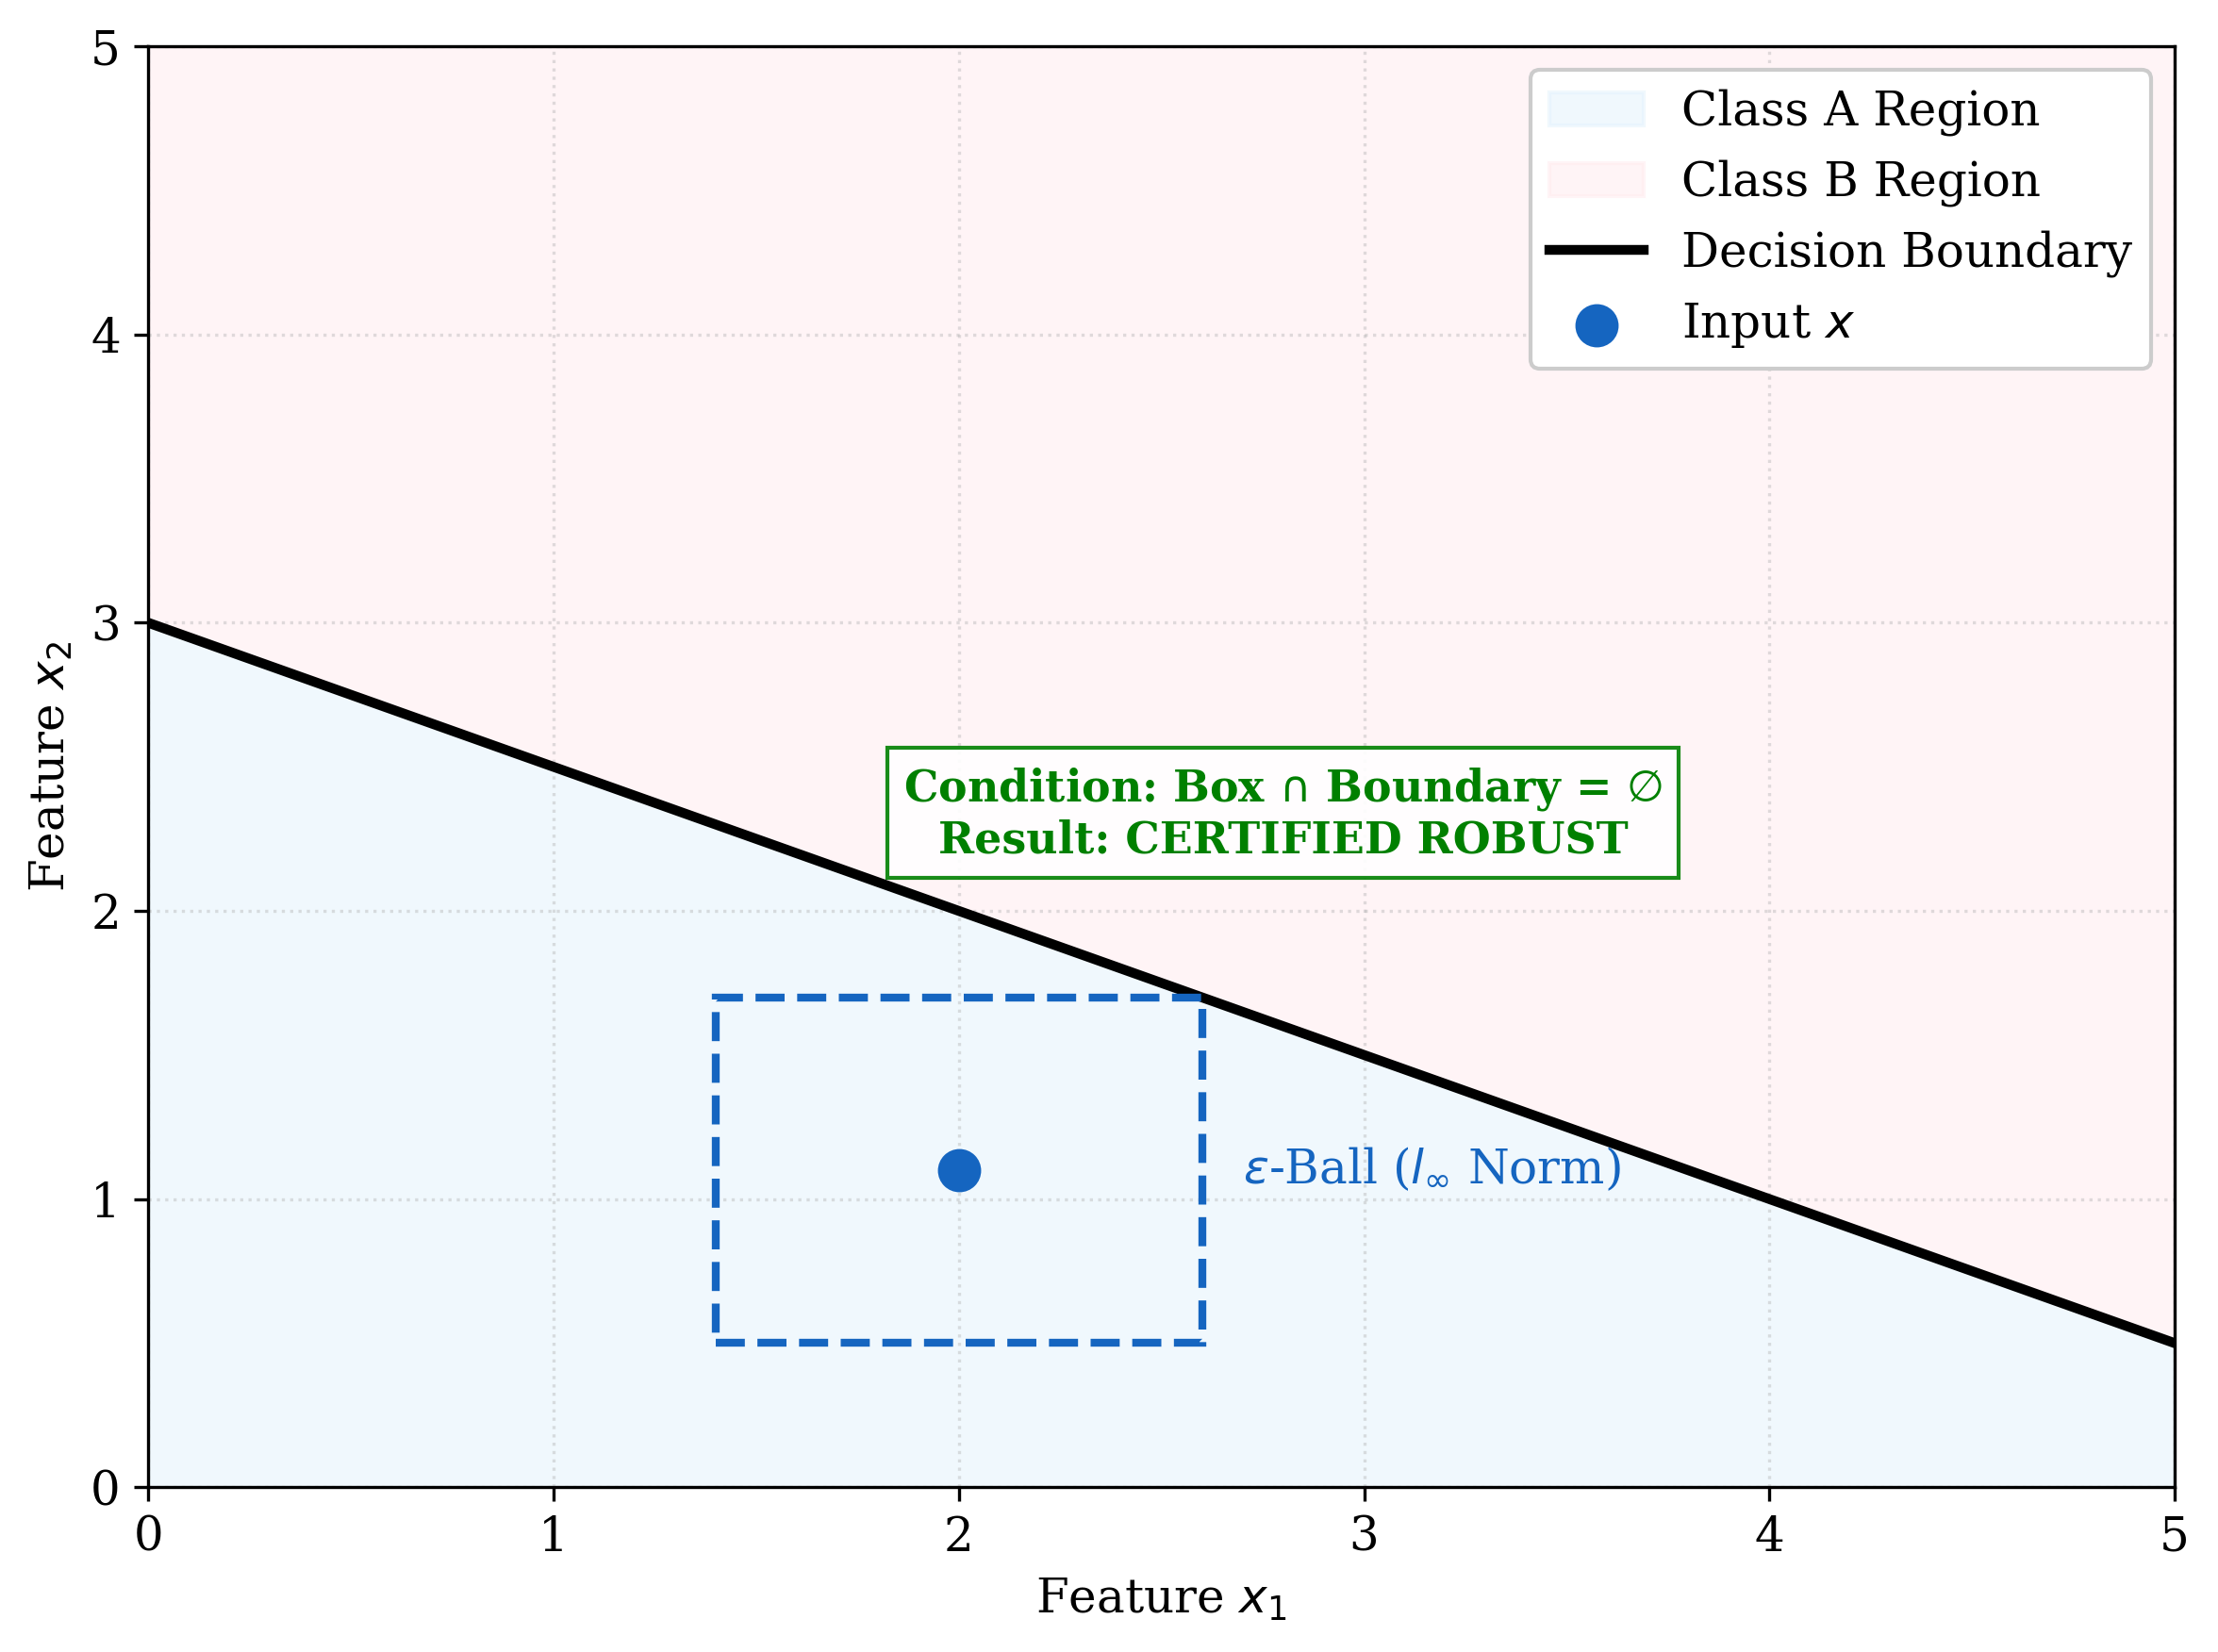
\includegraphics[width=0.8\textwidth]{figuras/2-fundamentos/safety/fig_why_uniform_linf.png}
    \caption{Example of $\ell_\infty$-norm ball}
    \label{fig:uniform_norm_verification}
    \end{figure}


\subsection{SMT Encoding}
In order to verify {QNNs} with bit-precision, the network must be transformed into a code problem rather than a model problem. As it will be embedded onto specific hardware, the first step is to transform the model into C code \cite{cordeiro2025neuralnetworkverificationprogramming}. Once in C code, the next step is to transform the constraints into a satisfiability problem, i.e., encode the neural network layer $f^{[l]}$ into an SMT formula that will verify if, by inputting a perturbation $\epsilon$, the known layer will be misclassified.

\begin{equation}
    \textbf{x}' = \textbf{x}+\epsilon,
\end{equation}
\begin{equation} \label{eq:safety_prop}
    \exists \, \textbf{x}' \in \mathcal{I} \rightarrow f'(\textbf{x}')\notin \mathcal{O}
\end{equation}

SMT solvers work by defining equations and constraints; we must write the safety property as a negation, i.e., a counterexample to be found. To use the Equation \ref{eq:safety_prop} with SMT solvers, it must be written as constraints:

\begin{align*}
\Phi_{\text{robust}}(\mathbf{x}, \epsilon) = & \exists \, \mathbf{x}' \in \mathcal{I} : \\
& \bigwedge_{i=1}^n (x_i - \epsilon \leq x'_i \leq x_i + \epsilon) \ \land \\
& \lnot (\arg\max \hat{f}(\mathbf{x}') \equiv \arg\max \hat{f}(\mathbf{x}))
\end{align*}
    
\begin{comment}
\subsubsection*{CEG4N}


\textbf{Neural Networks:} $\Gamma$ and $F$ \\
\textbf{Input Space:} $I \in \mathbb{R}^n$ \\
\textbf{Output Space:} $O \in \mathbb{R}^n$ \\

\textbf{Objective:} Prove that the mathematical functions of $\Gamma$ and $F$, $f:I \rightarrow O$ and $t:I\rightarrow O$, are equivalent.

\textbf{Equivalence:} Both NNs produce the same outputs for the same inputs.

\textbf{Definition 1 (Top-1-Equivalence):} Two NNs $f$ and $t$ are Top-1-equivalent if:
$$ \arg\max f(x) = \arg\max t(x), \forall x \in I $$

\textbf{Assumption 1:} For NN $F$ without quantization:
$$ \arg\max f(x) = y, \text{ for } x \in H $$

\textbf{Assumption 2:} For NN $F$ with quantization:
$$ \exists N \text{ such that } \arg\max f(x) = \arg\max f^q(x) = y, \forall x \in H $$



\textbf{Objective:} Maximize quantization while maintaining QNN equivalence to the floating point NN.

\textbf{Definition 2 (Robust Quantization):}
Let \( f \) be the reference NN and \( H \subset \mathbb{R}^n \) be a set of instances. Robust quantization is defined as:
\[ \text{Quantization of } f \text{ resulting in } f^q \text{ such that } \arg\max f(x) \Leftrightarrow \arg\max f^q(x), \forall x \in H \]

\textbf{Quantization Assumption:}
There exists a set \( N = \{n_1, n_2, \ldots, n_L\} \), where \( n_l \in N \) represents the number of bits for quantizing the \( l \)-th layer in \( f \).

\textbf{Robust Quantization Problem:}
Obtain a sequence of \( N \) where each \( n \in N \) is minimized, ensuring the equivalence between \( f \) and \( f^q \) is satisfied.


We consider the robust quantization of a neural network (NN) as an iterative minimization problem. Each iteration consists of two complementary sub-problems:

\begin{enumerate}
  \item Minimize the quantization bit widths by finding a candidate set \( N \).
  \item Verify the equivalence property, i.e., check if an NN quantized with the bit widths in \( N \) is equivalent to the original NN.
\end{enumerate}

\textbf{If the latter fails, we iteratively return to the minimization sub-problem with additional information.}

\begin{equation}
    N^o = \arg\min_{n_1,...,n_L} \sum_{l \in N_l <= L} n_l 
\end{equation}
    
$$
\begin{aligned}
& \arg\max f(x) = \arg\max f^q(x), & \forall x \in H^o_{CE} \\
& n_l \geq \underline{N} \vee n_l  \in N^o \\
& n_l  \leq \overline{N}  \vee n_l  \in N^o 
\end{aligned}
$$
    

Consider \( \overline{N} \) to be the upper limit and \( \underline{N} \) the lower one.
\begin{itemize}
  \item \( \overline{N} \) ensures two things:
  \begin{enumerate}
    \item It gives an upper bound to the quantization bit width.
    \item It provides a termination criterion. If a candidate \( N^o \) is found such that \( n_l = \overline{N} \) for every \( n_l \in N^o \), the optimization stops as it reaches Assumption 2.
  \end{enumerate}
  \item Assumption 2 ensures the termination of CEG4N, built on the premise that there exists a set of \( N \) where quantization introduces minimal error to the NN.
  \item If CEG4N proposes a quantization solution equal to \( \overline{N} \), this solution is verified, and if verification returns a counter-example, CEG4N finishes with failure.
  \item Note that \( H^o_{CE} \) is an iterative parameter, updated at each iteration based on the verification sub-problem.
\end{itemize}

In the Verification sub-problem $o$, we check whether the $N^o$ generated by the optimization sub-problem $o$ satisfies the following equivalence property:

\[\Psi(f,f^q, x,y)=\Psi_x(x)\rightarrow \Psi_y(y)\]

if  $\Psi_x(x)\rightarrow \Psi_y(y)$ holds for the candidate $N^o$, the optimization halts and $N^o$ is declared as solution; otherwise, a new counter-example $H_{CE}$ is generated. Iteration o+1 starts where iteration o stopped. That is, the optimization sub-problem o + 1 receives as parameter a set of $H^{+1}_{CE}$ such that $H^{o+1}_{CE}=H^o_{CE}\cup x_{CE}$.

    
    \subsection{Problem Encoding}
    
    \subsection{Neural Network Equivalence Problem}
    
    
    \subsection{Network Repair}
    
    Like said before, QNN are widely employed in human-activity. However, the quantization process can lead to a significant loss of accuracy. To address this issue, researchers have explored various techniques to repair quantized neural networks (QNNs).
    
    Repair NN have two main objectives: fix defects found in Neural Networks. It can be classified into three categories: retraining/fine-tuning, direct weight modification, and architecture extension \cite{song2023qnnrepair}.
    
    The equivalence problem is a fundamental challenge in the field of neural Network Repair. It shows that the equivalence problem can be reduced to a Satisfiability problem \cite{eleftheriadis2022neuralnetworkequivalencechecking}.
    
    
    
    
    \textcolor{red}
    {This approuch is not exclusive to QNNs.}
    
    \begin{itemize}
    \item AIREPAIR: A Repair Platform for Neural Networks
\end{itemize}

Reluplex: An Efficient SMT Solver for Verifying  Deep Neural Networks?

- This paper does not deal with quantized neural network
- Deep Neural Networks (DNN)
- It has been discovered that DNN can be disturbed even by the slighest pertubation
- Verifying DNN is a difficult problem. They are large, non-linear, and non convex.
- It's a NP-COMPLETE problem.
- LP Solvers and SMT solvers can be employed to verify DNN but until now have only be used to verify small Models.
- Activation function are a problem because they are non linear, thus the papers focus only in Relu
- It found out that some of RELU during search can be ignored.

Contribution
- Reluplex presents itself as a SMT solver for a theory of real time arithmetic with ReLu constrains

\end{comment}

%\textcolor{red}{can you add a table that compares your method with others from the literature?}

%\textcolor{red}{Can you add a summary section to describe the main findings?}

\section{The proposal work against state-of-the-art works}\label{sec:comparison_against_state_of_the_art}

In the work by Abdi et al.  \cite{abdi2021counterexample}, the authors present a method for quantizing a neural network that also uses ESBMC as a verification backend. Their approach is carried out as follows: (1) quantization bit-widths are initialized; (2) verification is performed with ESBMC, which may generate counterexamples ($\mathcal{H}_{CE}$); (3) these counterexamples are fed back to a Genetic Algorithm (GA) module; (4) the GA returns a new bit-width configuration for further testing. This iterative cycle continues to minimize bit-widths while ensuring equivalence between the baseline floating-point model and the quantized networks, in line with the goals of this work.


CEG4N was selected due to its similarities with this work: it employs ESBMC, which can switch SMT backends (including boolevector), and targets optimal bit-width. However, it does not factor adversarial attack robustness into quantization. Instead, it measures the quantized model against the floating-point baseline, treating the latter as robust. If the quantized model is NN-equivalent, it is also considered robust. The CEG4N framework was tested on small, fully connected NNs with the Iris and Seeds datasets. In these experiments, both the quantization similarity radius ($\epsilon$) and the dataset were varied. The reported results include the base ANN and quantized QNN accuracies, as well as verification time, summarized in Table~\ref{tab:ceg4n_results}. 



\begin{table}[!hb]
\centering
\caption{Results of quantization experiments.}
\label{tab:ceg4n_results}
\begin{tabular}{l c c c c c}
\hline
Dataset & Robustness Radius & Bit sequence &  ANN$_{acc}$ & QNN$_{acc}$ & Time (s)\\
\hline
iris\_10x2 &  0.01 &3-2-4 & 0.9000 & 0.9667 & 73 \\
iris\_10x2 &  0.03 &3-2-4 & 0.9000 & 0.9667 & 72 \\
iris\_10x2 &  0.05 &3-2-4 & 0.9667 & 0.9667 & 76 \\
\midrule
iris\_3x2 &  0.01 &2-3-4 & 0.9333 & 0.8667 & 8 \\
iris\_3x2 &  0.03 &2-3-4 & 0.9333 & 0.9000 & 8 \\
iris\_3x2 &  0.05 &2-3-4 & 0.9667 & 0.9667 & 10 \\
\midrule
seeds\_10x1 &  0.01 &3-3 & 0.9048 & 0.8810 & 74 \\
seeds\_10x1 &  0.03 &3-3 & 0.8571 & 0.8095 & 74 \\
seeds\_10x1 &  0.05 &3-3 & 0.9048 & 0.8333 & 72 \\
\midrule
seeds\_15x1 &  0.01 &3-3 & 0.9048 & 0.8571 & 124 \\
seeds\_15x1 &  0.03 &3-3 & 0.9048 & 0.8333 & 126 \\
seeds\_15x1 &  0.05 &3-3 & 0.9048 & 0.8571 & 130 \\
\midrule
seeds\_2x1 &  0.01 &4-4 & 0.8571 & 0.8571 & 9 \\
seeds\_2x1 &  0.03 &4-4 & 0.8571 & 0.8810 & 9 \\
seeds\_2x1 &  0.05 &4-4 & 0.8571 & 0.8333 & 9 \\
\midrule
seeds\_6x1 &  0.01 &4-2 & 0.8333 & 0.6905 & 36 \\
seeds\_6x1 &  0.03 &4-2 & 0.8095 & 0.6905 & 37 \\
seeds\_6x1 &  0.05 &4-2 & 0.8333 & 0.5714 & 37 \\
\hline
\end{tabular}
\end{table}

Our Framework, like CEG4N, was also evaluated using the same databases, as shown in Table \ref{tab:results-id25-esbmc-eps001003005}. We observe a clear speed-up compared to CEG4N because it treats the entire network as a single unit, thereby increasing complexity and the number of verification states.  Unlike our approach, which verifies each layer individually. This leads to fewer states for the ESBMC backend to process, making the verification task less demanding. As a result, we observe a clear speed-up compared to CEG4N. 

\begin{comment}
    
\begin{table}[htbp]
\centering
\caption{Results Using Our Proposed Methodology (Attack $\epsilon=0.01$, ID=25). Times in seconds.}
\label{tab:ours_framework_results}
\small
\begin{tabular}{@{}llccc rrr rr@{}}
\hline
Dataset & Backend & All bits & Backward & Forward & Time (s) & Acc. DNN & Acc. QNN \\
\hline
Iris\_10$\times$2 & ESBMC & {[4, 3, 3]} & 0.024 & 2.498 & 2.522 & 0.900 & 0.867 \\
Iris\_15$\times$2 & ESBMC & --- & --- & --- & 6.934 & --- & --- \\
Iris\_3$\times$2 & ESBMC & {[4, 4, 3]}  & 0.014 & 1.271 & 1.285 & 0.933 & 0.900 \\
Iris\_4$\times$2 & ESBMC & --- & --- & --- & 5.160 & --- & --- \\
Seeds\_10$\times$1 & ESBMC & {[7, 3]}  & 0.030 & 8.476 & 8.506 & 0.905 & 0.905 \\
Seeds\_15$\times$1 & ESBMC & {[7, 3]} & 0.060 & 24.926 & 24.986 & 0.905 & 0.905 \\
Seeds\_2$\times$1 & ESBMC & {[6, 4]} & 0.008 & 1.412 & 1.420 & 0.857 & 0.833 \\
Seeds\_4$\times$1 & ESBMC & ---  & --- & --- & 7.107 & --- & --- \\
Seeds\_5$\times$1 & ESBMC & {[6, 3]} & 0.011 & 2.219 & 2.230 & 0.833 & 0.833 \\
Seeds\_6$\times$1 & ESBMC & {[6, 3]} & 0.012 & 2.299 & 2.310 & 0.833 & 0.833 \\
\hline

\end{tabular}
\end{table}
\end{comment}
\newpage
\begin{table}[!htbp]
\centering
\caption{Resultados de quantização e verificação usando ESBMC (ID=25). Tempos em segundos.}
\label{tab:results-id25-esbmc-eps001003005}
\scriptsize
\resizebox{\linewidth}{!}{%
\begin{tabular}{@{}lc ccc rrr cc@{}}
\toprule
Dataset & $\epsilon$ & All bits & Frac bits & Int bits & Backward & Forward & Total & Acc.\ DNN & Acc.\ QNN \\
\midrule
Iris\_10x2 & 0.01 & {[4, 3, 3]} & {[2, 1, 1]} & {[2, 2, 2]} & 0.028 & 2.984 & 3.012 & 0.900 & 0.867 \\
Iris\_10x2 & 0.03 & {[4, 3, 3]} & {[2, 1, 1]} & {[2, 2, 2]} & 0.031 & 2.995 & 3.026 & 0.900 & 0.867 \\
Iris\_10x2 & 0.05 & {[4, 5, 3]} & {[2, 3, 1]} & {[2, 2, 2]} & 0.053 & 6.457 & 6.510 & 0.900 & 0.867 \\
\midrule
Iris\_3x2 & 0.01 & {[4, 4, 3]} & {[2, 1, 1]} & {[2, 3, 2]} & 0.021 & 0.935 & 0.956 & 0.933 & 0.900 \\
Iris\_3x2 & 0.03 & {[4, 4, 3]} & {[2, 1, 1]} & {[2, 3, 2]} & 0.021 & 0.895 & 0.916 & 0.933 & 0.900 \\
Iris\_3x2 & 0.05 & {[4, 4, 3]} & {[2, 1, 1]} & {[2, 3, 2]} & 0.039 & 1.746 & 1.785 & 0.933 & 0.900 \\
\midrule
Seeds\_10x1 & 0.01 & {[7, 3]} & {[5, 1]} & {[2, 2]} & 0.012 & 4.272 & 4.284 & 0.905 & 0.905 \\
Seeds\_10x1 & 0.03 & {[7, 3]} & {[5, 1]} & {[2, 2]} & 0.011 & 5.744 & 5.755 & 0.905 & 0.905 \\
Seeds\_10x1 & 0.05 & {[7, 3]} & {[5, 1]} & {[2, 2]} & 0.025 & 12.877 & 12.902 & 0.905 & 0.905 \\
\midrule
Seeds\_15x1 & 0.01 & {[7, 3]} & {[5, 1]} & {[2, 2]} & 0.013 & 9.272 & 9.285 & 0.905 & 0.905 \\
Seeds\_15x1 & 0.03 & {[9, 3]} & {[7, 1]} & {[2, 2]} & 0.014 & 47.655 & 47.669 & 0.905 & 0.905 \\
Seeds\_15x1 & 0.05 & - & - & - & - & - & 1534.478 & - & - \\
\midrule
Seeds\_2x1 & 0.01 & {[6, 4]} & {[3, 1]} & {[3, 3]} & 0.010 & 1.076 & 1.086 & 0.857 & 0.833 \\
Seeds\_2x1 & 0.03 & {[6, 4]} & {[3, 1]} & {[3, 3]} & 0.010 & 1.084 & 1.093 & 0.857 & 0.833 \\
Seeds\_2x1 & 0.05 & {[6, 4]} & {[3, 1]} & {[3, 3]} & 0.021 & 1.931 & 1.952 & 0.857 & 0.833 \\
\midrule
Seeds\_5x1 & 0.01 & {[6, 3]} & {[4, 1]} & {[2, 2]} & 0.012 & 1.920 & 1.932 & 0.833 & 0.833 \\
Seeds\_5x1 & 0.03 & {[7, 3]} & {[5, 1]} & {[2, 2]} & 0.013 & 2.437 & 2.450 & 0.833 & 0.833 \\
Seeds\_5x1 & 0.05 & {[9, 3]} & {[7, 1]} & {[2, 2]} & 0.018 & 8.157 & 8.175 & 0.833 & 0.857 \\
\midrule
Seeds\_6x1 & 0.01 & {[6, 3]} & {[4, 1]} & {[2, 2]} & 0.013 & 2.154 & 2.167 & 0.833 & 0.833 \\
Seeds\_6x1 & 0.03 & {[7, 3]} & {[5, 1]} & {[2, 2]} & 0.012 & 2.423 & 2.434 & 0.833 & 0.833 \\
Seeds\_6x1 & 0.05 & {[9, 3]} & {[7, 1]} & {[2, 2]} & 0.018 & 8.310 & 8.328 & 0.833 & 0.857 \\
\bottomrule
\end{tabular}%
}
\end{table}


\subsubsection*{Summary}\label{sub}
Table~\ref{tab:comparison_esbmc_ceg4n} shows the comparison of our method to other state-of-the-art frameworks aiming to find optimal quantization bit-widths, such as CEG4N. The comparison includes quantization bit-widths, verification times, and accuracies for both original and quantized networks. Our strategy achieves quantization that is comparable or better while upholding accuracy. It also provides reduced verification times in several cases, demonstrating greater computational efficiency for the quantization process.


\newpage
%$x_i \in \mathcal{Y} \quad \forall$ $i \in \mathcal{I}$
\begin{table}[!htbp]
\centering
\caption{Comparison of quantization results: Proposed vs. CEG4N. \textbf{Acc} denotes the accuracy of the Quantized Neural Network (QNN). Time is in seconds.}
\label{tab:comparison_esbmc_ceg4n}
\scriptsize
\setlength{\tabcolsep}{3pt} % Reduce column padding to fit width
\resizebox{\linewidth}{!}{%
\begin{tabular}{@{}ll | ccc | ccc@{}}
\toprule
\multicolumn{2}{c}{} & \multicolumn{3}{c}{\textbf{(Proposed)}} & \multicolumn{3}{c}{\textbf{CEG4N}} \\
\cmidrule(lr){3-5} \cmidrule(l){6-8}
Dataset & $\epsilon$ & Bits & Acc. & Time (s) & Bits & Acc. & Time (s) \\
\midrule

\multirow{3}{*}{Iris\_10x2} 
 & 0.01 & [4, 3, 3] & 0.867 & \textbf{3.01} & 3-2-4 & \textbf{0.967} & 73 \\
 & 0.03 & [4, 3, 3] & 0.867 & \textbf{3.03} & 3-2-4 & \textbf{0.967} & 72 \\
 & 0.05 & [4, 5, 3] & 0.867 & \textbf{6.51} & 3-2-4 & \textbf{0.967} & 76 \\
\midrule

\multirow{3}{*}{Iris\_3x2} 
 & 0.01 & [4, 4, 3] & \textbf{0.900} & \textbf{0.96} & 2-3-4 & 0.867 & 8 \\
 & 0.03 & [4, 4, 3] & 0.900 & \textbf{0.92} & 2-3-4 & 0.900 & 8 \\
 & 0.05 & [4, 4, 3] & 0.900 & \textbf{1.79} & 2-3-4 & \textbf{0.967} & 10 \\
\midrule

\multirow{3}{*}{Seeds\_10x1} 
 & 0.01 & [7, 3] & \textbf{0.905} & \textbf{4.28} & 3-3 & 0.881 & 74 \\
 & 0.03 & [7, 3] & \textbf{0.905} & \textbf{5.76} & 3-3 & 0.810 & 74 \\
 & 0.05 & [7, 3] & \textbf{0.905} & \textbf{12.90} & 3-3 & 0.833 & 72 \\
\midrule

\multirow{3}{*}{Seeds\_15x1} 
 & 0.01 & [7, 3] & \textbf{0.905} & \textbf{9.29} & 3-3 & 0.857 & 124 \\
 & 0.03 & [9, 3] & \textbf{0.905} & \textbf{47.67} & 3-3 & 0.833 & 126 \\
 & 0.05 & - & - & 1534.5 & 3-3 & \textbf{0.857} & \textbf{130} \\
\midrule

\multirow{3}{*}{Seeds\_2x1} 
 & 0.01 & [6, 4] & 0.833 & \textbf{1.09} & 4-4 & \textbf{0.857} & 9 \\
 & 0.03 & [6, 4] & 0.833 & \textbf{1.09} & 4-4 & \textbf{0.881} & 9 \\
 & 0.05 & [6, 4] & \textbf{0.833} & \textbf{1.95} & 4-4 & \textbf{0.833} & 9 \\
\midrule

\multirow{3}{*}{Seeds\_6x1} 
 & 0.01 & [6, 3] & \textbf{0.833} & \textbf{2.17} & 4-2 & 0.691 & 36 \\
 & 0.03 & [7, 3] & \textbf{0.833} & \textbf{2.43} & 4-2 & 0.691 & 37 \\
 & 0.05 & [9, 3] & \textbf{0.857} & \textbf{8.33} & 4-2 & 0.571 & 37 \\

\bottomrule
\end{tabular}%
}
\end{table}

\chapter{Methodology}\label{chap:methodology}

In this chapter, we will detail the pillar of our proposed methodology for our end-to-end framework that aims to find the optimal bit-width for each layer of QNN while ensuring that the defined bit-widths satisfy robustness properties using the SMT Theory of Fixed-Point Arithmetic.

%replaced by below
%This work is based on Cai et al.'s framework called Quadapter \cite{cai2025certified}, a framework for synthesizing QNN that are robust against adversarial attack using MILP solvers. However, unlike Quadapter, which relies on idealized mathematical models, our approach aims to incorporate the SMT Theory of Fixed-Point Arithmetic to ensure that the synthesized QNNs are verified under finite-precision arithmetic.

%Our work is based on Cai et al.'s Quadapter \cite{cai2025certified}, which synthesizes a QNN from a regular floating-point precision ANN to keep it robust against adversarial attacks by using MILP solver to verify for vulnerabilties and thus use the information to find the best bit-width for quantization. However, unlike his work, ours aims to incorporate the SMT Theory of verifying Fixed-point arithmetic to ensure that the found QNN is also verified under finite-precision arithmetic.
Our work is built upon Cai et al.'s Quadapter \cite{cai2025certified}, which aims to convert a traditional floating-point Neural Network into a similar fixed-point QNN with an enhanced robustness against adversarial attacks within the quantized model. This is achieved by employing an MILP solver to identify vulnerabilities and determine the optimal quantization bit-width for each layer. In contrast, our approach integrates an SMT solver to verify the defined constraints, accounting for the particulars of fixed-point arithmetic, thereby ensuring that the resulting QNN is rigorously validated under finite-precision arithmetic constraints \cite{baranowski2020smt}.

%Similarly, Quadapter, our framework, also computes the preimage of each ANN layer and uses it to define the optimal bit-width for each layer $\xi_{i}$, while ensuring that the robustness property is satisfied. The safety property will be verified using an off-the-shelf SMT-based verifier, such as ESBMC \cite{esbmc2025}, that supports fixed-point arithmetic.
Similarly to Quadapter, our framework, also computes the preimage of each ANN layer and uses it to define the optimal bit-width for each layer $\xi_{i}$ by selecting the best set that ensures the robustness property is satisfied. The safety property is verified using an off-the-shelf SMT-based verifier, ESBMC \cite{esbmc2025}, that supports fixed-point arithmetic.

The general methodology of our proposed framework is summarized in the diagram shown in Figure \ref{fig:diagrama_metodologia} and detailed in the Algorithm \ref{alg:quantization_synthesis}.

\newpage
\begin{comment}
    
\begin{figure}[!hb]
\centering
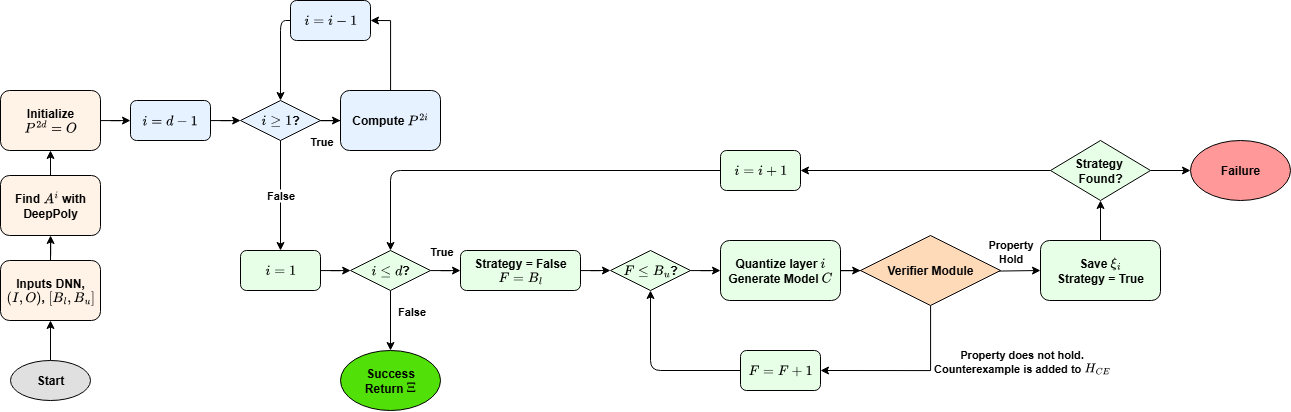
\includegraphics[width=1\textwidth]{figuras/3-metodologia/diagram_v1.png
}
\caption{Proposed Methodology Diagram}
\label{fig:diagrama_metodologia}
\end{figure}
\end{comment}

\begin{figure}[!hb]
\centering
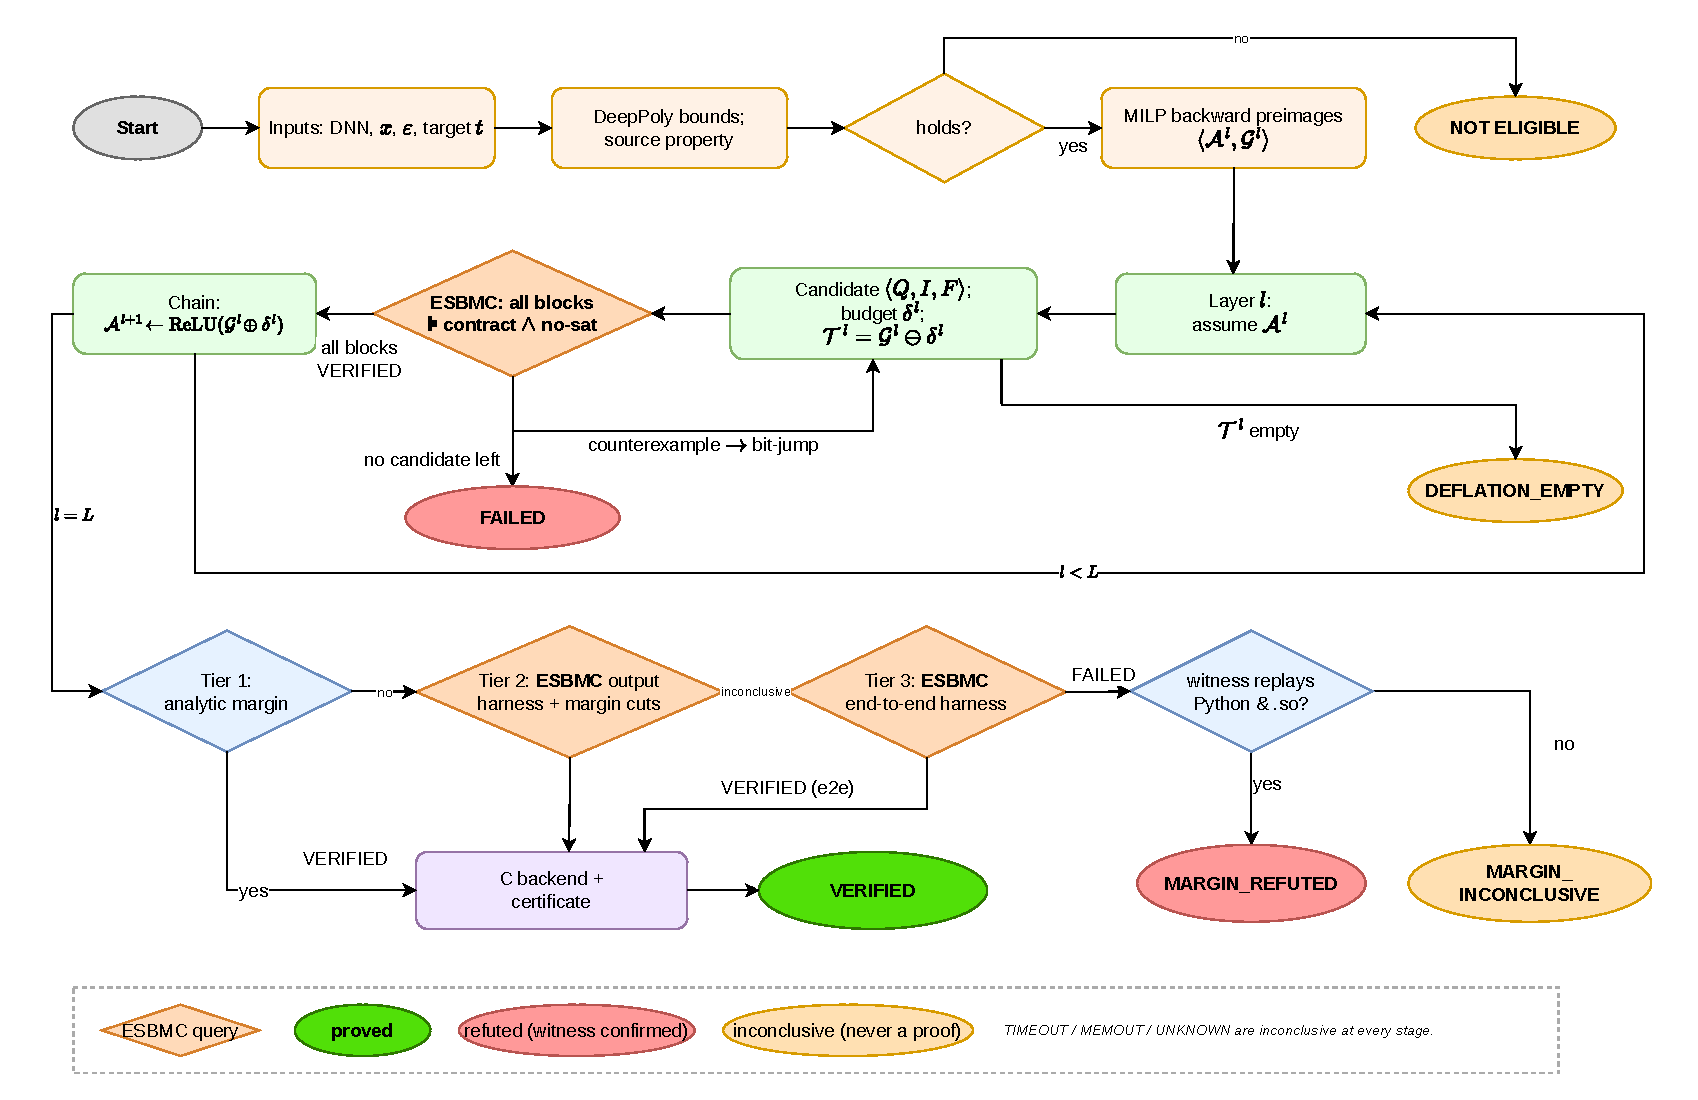
\includegraphics[width=1\textwidth]{figuras/3-metodologia/main_diagram_preqbmc_pdf.drawio.pdf}


\caption{Proposed Methodology Diagram}
\label{fig:diagrama_metodologia}

\end{figure}

%We call the original ANN as $\mathcal{N}$ and the quantized neural network as ${\hat{\mathcal N}}$. The layers of the ANN are represented as $f_i$ and the layers of the QNN as $\hat{f_i}$. The preimage of each layer $f_i$ is represented as $P_i$ and it represents the under-approximation $P^{2l} \subseteq \mathcal N^{1:2i}_{2i}(\mathcal O)$. Our approach decomposes this global verification problem into a series of layer-wise counter-example verification problems. Specifically, for each affine layer $f_{2i}$. Initially, we use the DeepPoly \cite{singhAbstractDomainCertifying2019} abstract interpretation framework to prove that the original floating-point DNN satisfies the robustness property and to compute admissible output intervals for each layer, $\mathcal{A}^i_{j}$. Next, we perform a backward preimage computation to derive output intervals for each layer that are sufficient to guarantee the overall robustness property. These intervals are defined by $P^{2l}$ and will be used to guide the synthesis of the QNN. Then, for each layer independently, we verify that its quantized counterpart $\hat{f_{2i}}$ satisfies the property shown in Equation \ref{eq:main_preposition_milp} which ensures that the quantized affine layer's output falls within the calculated preimage, thus implying that the entire quantized network $\hat{N}$ satisfies the global robustness property defined.
We call the original ANN as $\mathcal{N}$ and the quantized neural network as ${\hat{\mathcal N}}$. The layers of the ANN are represented as $f^{[l]}$ and the layers of the QNN as $\hat{f^{[l]}}$. The preimage of each layer $f^{[l]}$ is represented as $P_i$ and it represents the under-approximation $P^{2[l]} \subseteq \mathcal N^{1:2[l]}_{2[l]}(\mathcal O)$. Our approach decomposes this global verification problem into a series of layer-wise counter-example verification problems. Specifically, for each affine layer $f^{2[l]}$. Initially, we use the DeepPoly \cite{singhAbstractDomainCertifying2019} abstract interpretation framework to prove that the original floating-point ANN satisfies the robustness property and to compute admissible output intervals for each layer, $\mathcal{A}^{[l]}_{j}$. Next, we perform a backward preimage computation to derive output intervals for each layer that are sufficient to guarantee the overall robustness property. These intervals are defined by $P^{2[l]}$ and will be used to guide the synthesis of the QNN. For each affine quantized layer, $\hat{f^{2[l]}}$, we verify whether the condition in equation \ref{eq:main_preposition_milp} holds. By confirming this property at every layer, we establish that the entire $\mathcal{ \hat{N}}$ satisfies the global robustness property.


\begin{equation}\label{eq:main_preposition_milp}
    %\hat{N}^{1:2[l]}_{2[l]}(\mathcal I) \subseteq P^{2[l]} \implies \hat{N} \vDash <\mathcal I, \mathcal O>
\hat{\mathcal{N}}^{1:2[l]}_{2[l]}(\mathcal{I}) \subseteq P^{2[l]} \implies \hat{\mathcal{N}} \models \langle \mathcal{I}, \mathcal{O} \rangle
\end{equation}

%% Algorithm
\begin{algorithm}[H]
\caption{SMT-Based Quantization Synthesis for Robust Neural Networks}
\label{alg:quantization_synthesis}
\begin{algorithmic}[1]
\Require Original network $\mathcal N$, input region $\mathcal{I}$, output region $\mathcal{O}$, bit-width search space $\Xi$
\Ensure Quantized network $\mathcal{\hat{N}}$ satisfying robustness property, or synthesis failure
\State \textbf{Phase 1:} Compute $\mathcal{A}^{[l]}_{j}$ using DeepPoly and backward preimage $P^{2l}$ from $\mathcal{O}$
\For{each affine layer $f^{2[l]} \in \mathcal N$}
    \For{each bit-width configuration $\xi_{[l]} \in \Xi$}
        \State Quantize $\mathbf{W}^{2[l]}, \mathbf{b}_{2l}$ with $\xi_{[l]} = \langle Q_{[l]}, F_{[l]} \rangle$
        \State Generate C harness for $\hat{f}^{2[l]}$ with fixed-point arithmetic
        \State Encode constraint $\mathcal{\hat{N}}^{1:2[l]}_{2[l]}(\mathcal{I}) \subseteq P^{2[l]}$ as SMT assertions
        \State $\text{result} \gets$ \Call{ESBMC-Verify}{C harness, timeout}
        \If{$\text{result} = \textsc{Verified}$}
            \State Record $\xi_{[l]}^* \gets \xi_{[l]}$ and \textbf{break}
        \EndIf
    \EndFor
    \If{no verified configuration found}
        \State \Return \textsc{Synthesis-Failure} for layer $[l]$
    \EndIf
\EndFor
\State \textbf{return} $\hat{N}$ with $\Xi = \{\xi_1^*, \xi_2^*, \ldots, \xi_d^*\}$
\end{algorithmic}
\end{algorithm}

\section{Input Region Definition and Initialization}
% Text below had indices of AI usage. We will fix it.
%The verification process begins by defining the input uncertainty region in the main entry point of the program. Given the input $x$ $\forall$ $\in$ $\mathbb{R}^n$ and the pertubation $\delta$ such that $||\delta||_\infty \leq \epsilon$, we define the input bounds as follows: $x_{low} = clip(x - \epsilon)$ and $x_{high} = clip( x + \epsilon)$, where the clip function ensures that the extubated inputs remain within the valid input range domain. For datasets like iris and seeds, the dataset perturbation is determined by the natural features of the data. \textcolor{blue}{For example for the iris dataset or seeds one the addition of $\epsilon$ could not make sense, as $0.01$ could not be enough to be considered a significant perturbation. Thus, for these datasets, we define a normalized perturbation based on the standard deviation of each feature in the dataset.}



The verification procedure starts by defining an uncertainty region around the input at the program's main entry point. Let $x \in \mathbb{R}^n$ be the nominal input and let $\delta$ be a perturbation such that $\lVert \delta \rVert_\infty \leq \epsilon$. From this, we obtain lower and upper bounds for the input:
\begin{equation}
    x_{\text{low}} = \operatorname{clip}(x - \epsilon),
    \qquad
    x_{\text{high}} = \operatorname{clip}(x + \epsilon),
\end{equation}
where the function $\operatorname{clip}(\cdot)$ keeps each feature inside its valid range.

For image-like data, using a fixed $\epsilon$ in the original scale is usually reasonable, because all features share a similar range. For tabular data, however, this is not always the case. In datasets such as \textit{Iris} or \textit{Seeds}, different features can have very different scales, so a small value like $\epsilon = 0.01$ may be almost irrelevant for some features and too strong for others. To avoid this issue, we use a feature-wise normalized perturbation based on each feature's standard deviation. For each feature $j$, we define
\begin{equation}
    \epsilon_j = \kappa \sigma_j,
\end{equation}
where $\sigma_j$ is the standard deviation of feature $j$ in the dataset and $\kappa$ is a user-defined factor that controls the size of the perturbation. The bounds are then computed as
\begin{equation}
    x_{\text{low}} = \operatorname{clip}(x - \epsilon_j),
    \qquad
    x_{\text{high}} = \operatorname{clip}(x + \epsilon_j),
\end{equation}
with $\epsilon = (\epsilon_1, \dots, \epsilon_n)$.


\begin{comment}
    As explained in the paragraph before, the use of just a variable does not make sense as for some dataset the variable may influence a lot bot for other it may just be a insignificant change. Thus, we have some options as below:
        - Make the normalization based on the standard deviation of each feature in the dataset.

\end{comment}

\section{Symbolic Bound Propagation}
%With the input region defined by $\mathcal{I}$, the DeepPoly abstract interpretation framework is instantiated to compute the concrete lower and upper bounds for every neural of ANN. It performs a forward pass through the network, maintaining  symbolic linear constraints that express each neuron's activation as a function of the input variables like shown in Figure \ref{fig:preimage_backpropagation}. For each affine layer transformation, DeepPoly computes both concrete bounds and symbolic bounds and the symbolic constraints that relate the output to the input.

%The results of this propagation are stored in the layer structures of the network. For each $f_i$, the framework maintain several sets of bounds: $l_i$ and $u_i$ represent respectively the concrete lower and upper bounds of the affine $i$ layer outputs.
With the input region defined by $\mathcal{I}$, the DeepPoly abstract interpretation framework is instantiated to compute the concrete lower and upper bounds for every neural network of ANN. It performs a forward pass through the network, maintaining  symbolic linear constraints that express each neuron's activation as a function of the input variables, as shown in Figure \ref{fig:preimage_backpropagation}. For each affine-layer transformation, DeepPoly computes both concrete and symbolic bounds, as well as the symbolic constraints relating the output to the input.

The results of this propagation are stored in the network's layer structures. For each $f^{[l]}$, the framework maintains several sets of bounds: $l_i$ and $u_i$ represent the concrete lower and upper bounds of the affine $i$ layer outputs.

\section{Backward Preimage Computation}
%The backward image computation is crucial for decomposing the global verification problem into a layer-wise sub-problem. By knowing the desired output region $\mathcal{O}$ of output layer, we compute the under-approximation of the preimage $P^{2d}$ for each affine layer $f^{2i}$. This preimage represents the set of output domain of each layer, thus by knowing that the output of last layer is $\mathcal{O}$, we can compute the preimage of the last affine layer $P^{2d}$ and then use it to compute the preimage of the previous layer $P^{2(d-1)}$ and so on until reaching the first layer $P^{0}$. The preimage is also computed to the activation layers by propagating the preimage through the activation functions to later use it in the verification of the next affine layer.

%This backward propagation is conservative in the sense that the computed preimages may be smaller than strictly necessary, but it guarantees that if the quantized layer's output falls within this preimage, then all the subsequent layers will also behave correctly. This conservatism is essential for ensuring the soundness of the layer-wise verification approach \textcolor{red}{WHY???}. The preimage intervals serve as the verification targets during the subsequent ESBMC verification step for each quantized layer.
The backward image computation is crucial for decomposing the global verification problem into a layer-wise sub-problem. By knowing the desired output region $\mathcal{O}$ of the output layer, we compute the under-approximation of the preimage $P^{2d}$ for each affine layer $f^{2[l]}$. This preimage represents the set of output domain of each layer, thus by knowing that the output of last layer is $\mathcal{O}$, we can compute the preimage of the last affine layer $P^{2d}$ and then use it to compute the preimage of the previous layer $P^{2(d-1)}$ and so on until reaching the first layer $P^{0}$. The preimage is also computed for the activation layers by propagating it through the activation functions for later use in verifying the next affine layer.

The mentioned backward calculation of the preimage is conservative, i.e., an underapproximation of the real region; thus, it may represent a smaller region than strictly necessary, but it guarantees that if the quantized layer is within its bounds, all subsequent layers will also behave correctly. The preimage intervals serve as the verification targets during the subsequent ESBMC verification step for each quantized layer.
\begin{figure}[!hb]
\centering
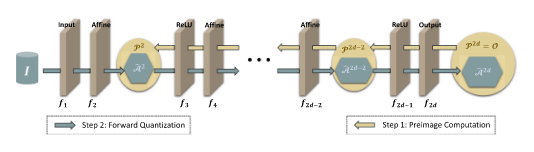
\includegraphics[width=0.8\textwidth]{figuras/3-metodologia/preimage_backpropagation.png} 
\caption{Backpropagation of Preimage through the Network Layers \cite{cai2025certified}}
\label{fig:preimage_backpropagation}
\end{figure}

\section{Quantization Search with ESBMC}
\begin{comment}
    
$The method implements the core quantization verification loop, systematically searching for the optimal bit-width configuration $\mathcal <Q, F\mathcal>$ where  $Q$ is the total bit-width and $F$ is the number of fractional bits for each layer that ensures the satisfaction of the robustness property.  The method iterates over each affine layer of the network until reach the output, and for each layer, it explores a range of bit-width, the method tries different divisions between integer and fractional bits to find the optimal configuration. Once found the configuration $\xi _{i}$ for layer $i$, it is fixed and the method proceeds to the next layer. The set of possible solutions is defined as $\varXi = {\{\xi _1, \xi _2, ..., \xi _{d}\}}$ where $d$ is the number of layers. 

$For a given configuration, the layer's weight and biases are quantized by scaling them by $2^{fractional\_bits}$ and rounding to the nearest integer: $round(weight * 2^{fractional\_bits})$ and $round(bias * 2^{fractional\_bits})$. This quantization scheme represents values in QF format, where arithmetic operation are performed on integers that implicitly represent fixed-point numbers with $F$ fractional bits. 

$The search strategy is greedy as for each layer the method tries bit-widths from the smallest to largest, and for each bit-width, it tries configurations with different fractional bit allocations. As soon as ESBMC successfully verifies a passing configuration, the method records this configuration and moves to the next layer. If no configuration passes for a given layer, the method raises an exception indicating that the quantization synthesis has failed for the network.
\end{comment}

The method implements the core quantization verification loop, systematically searching for the optimal bit-width configuration $\mathcal <Q, F\mathcal>$ where  $Q$ is the total bit-width and $F$ is the number of fractional bits per layer that ensures the satisfaction of the robustness property.  The method iterates over each affine layer of the network until it reaches the output, and for each layer, it explores a range of bit-width. The method tries different divisions between integer and fractional bits to find the optimal configuration. Once found, the configuration $\xi _{[l]}$ for layer $i$ it is fixed, and the method proceeds to the next layer. The set of possible solutions is defined as $\varXi = {\{\xi _1, \xi _2, ..., \xi _{d}\}}$ where $d$ is the number of layers. 

For a given configuration, the layer's weight and biases are quantized by scaling them by $2^{fractional\_bits}$ and rounding to the nearest integer: $round(weight * 2^{fractional\_bits})$ and $round(bias * 2^{fractional\_bits})$. This quantization scheme represents values in QF format, where arithmetic operations are performed on integers that implicitly represent fixed-point numbers with $F$ fractional bits. 

The search strategy is greedy: for each layer, the method tries bit-widths from the smallest to largest, and for each bit-width, it tries configurations with different fractional bit allocations. As soon as ESBMC successfully verifies a passing configuration, it records the configuration and proceeds to the next layer. If no configuration passes for a given layer, the method throws an exception indicating that the quantization synthesis has failed for the network.

\subsection{QNN Code Generation}
\begin{comment}
    - Usually ANN are thought as mathematical functions, but in reality they are implemented in HW as source code of a certain language. Thus, we can think it as a code verification problem.
    - We use C Language as an abstraction of QNN implementation
\end{comment}
%In the Machine Learning community, ANNs are typically represented as mathematical functions that map the input space to the outer space through a series of layers and activation functions. Our work, rather than focusing on the mathematical representation of ANNs, adopts a code-centric perspective, viewing ANNs as programs implemented in a C programming language. Thus, we approach the verification of the ANNs as a code verification problem like proposed by other works such as Cordeiro et al. \cite{cordeiro2025neuralnetworkverificationprogramming} and Sena et al. \cite{abdi2021counterexample}.
In the Machine Learning community, ANNs are typically represented as mathematical functions that map the input space to the outer space through a series of layers and activation functions. Our work, rather than focusing on the mathematical representation of ANNs, adopts a code-centric perspective, treating ANNs as programs implemented in the C programming language. Thus, we approach the verification of the ANNs as a code verification problem, as proposed by other works as Sena et al. \cite{abdi2021counterexample} and subsequently Cordeiro et al. \cite{cordeiro2025neuralnetworkverificationprogramming}.
\subsection{Introducing Safety Properties in ANN Code}\label{sec:safety_prop}

%As described before, we intend to use the SMT Theory to verify safety properties in QNNs. To do so, we will follow the approach proposed by Cordeiro et al. \cite{cordeiro2025neuralnetworkverificationprogramming} that consists of translating the neural network and the safety property into a C program. This program can then be verified using an SMT-based verifier like ESBMC \cite{esbmc2025}.

%Since the Bound Model Check technique used by ESBMC explores all possible execution paths of the program up to a certain depth, it was necessary to make use of non-deterministic variables to represent the inputs of the neural network. This allows ESBMC to explore all possible input combinations and verify if the safety property holds to all possible inputs. Thus, the first step in our methodology is to define the input variables of the neural network as non-deterministic variables in the C code. This can be done using the following notation:
As described before, we intend to use the SMT Theory to verify safety properties in QNNs. To do so, we follow the approach proposed by Cordeiro et al. \cite{cordeiro2025neuralnetworkverificationprogramming} that consists of translating the neural network and the safety property into a C program. This program can then be verified using an SMT-based verifier like ESBMC \cite{esbmc2025}.

Since the Bound Model Check technique used by ESBMC explores all possible execution paths of the program up to a given k-depth, it was necessary to use nondeterministic variables to represent the neural network’s input. This allows ESBMC to explore all possible input combinations and verify if the safety property holds for an n-set of possible inputs. Thus, the first step in our methodology is to define the neural network's input variables as nondeterministic in the C code. This can be done using the following notation:
\begin{equation}
    \begin{aligned}
    \texttt{in\_[j] = nondet\_longlong();}
    \end{aligned}
\end{equation}

%Let's consider the robustness property as an example. To verify if a neural network is robust against adversarial attacks within a certain radius $\epsilon$ under the $\ell^\infty$ norm, we need to ensure that for any input $x$ and any perturbation $\delta$ such that $||\delta||_\infty \leq \epsilon$, the output of the neural network remains unchanged. Consequently, we encode the premise with precondition assertions that define the input space and the pertubation limits within the bound of the original ANN. \textcolor{red}{Explain the perturbation is already included in the input bounds}
To verify if a neural network is robust, we are considering a perturbation radius $\epsilon$ under the $\ell^\infty$ norm. In resume: we need to ensure that for any input $x$, and any perturbation $\delta$ such that $||\delta||_\infty \leq \epsilon$, the output of the QNN will remain unchanged. Consequently, we encode the premise as precondition assertions that define the input space and the perturbation limits within the original ANN's bounds. 
\begin{equation}
    \begin{aligned}
    \texttt{\_\_ESBMC\_assume(in\_[j] >= input\_bounds\_low[j] \&\&} \\
    \texttt{in\_[j] <= input\_bounds\_high[j]);}
    \end{aligned}
\end{equation}

This notation ensures that the SMT solver only considers input within the specified assumption bounds. Next, we need to encode the conclusion of the robustness property using post-condition assertions that check if the output of the neural network remains unchanged for all perturbed inputs within the defined bounds by checking for a counter-example, i.e., if there exists an output that falls outside the expected range defined by the preimage of the output layer.


\begin{equation}
    \begin{aligned}
    \texttt{\_\_ESBMC\_assert(s\_out >= pre\_lo - eps \&\& s\_out <= pre\_hi + eps)}
    \end{aligned}
\end{equation}
%%%%%%%%%%%%%%%%%%%%%%%%%%%%%%%%% STOPPED Verifing Here
In case of ESBMC finding a counter-example, i.e., an example that violates the defined assertion, it would indicate by the definition of the assertion that the QNN is not robust, thus the $\xi _{x}$ configuration is not safe, therefore it must dismiss that configuration and try with another one until no counter-example is found. Conversely, if no counter-example is found within the specified bounds, it confirms that the QNN maintains its robustness property under the defined perturbations. 

\section{ESBMC Execution}
The framework calls for the ESBMC instance tool version 7.11 to verify the safety property on the generated C harness and to interpret the results. ESBMC is invoked with a carefully chosen set of command-line options that balance verification power with execution time. 

\begin{itemize}
    \item \texttt{-{}-boolevectors} chooses the Boolevector solver as it shows better performance in previous works \cite{li2025esbmcv76enhancedmodel}.
    \item \texttt{-{}-ir} use of integral/real arithmetic for fixed-point operations verification.
    \item \texttt{-{}-loop-invariant} enables loop invariant generation, which can help ESBMC reason about loops more effectively.
    \item \texttt{--incremental-bmc} enables incremental bounded model checking, which can improve performance by reusing solver state across different unrolling depths.
    \item \texttt{-{}-interval-analysis} activates interval analysis to compute variable bounds, aiding in pruning infeasible paths.
    \item \texttt{--no-unwinding-assertions} disables unwinding assertions to reduce overhead when loops are fully unrolled.
    \item \texttt{-{}-state-hashing} enables state hashing to avoid redundant exploration of identical program states.
\end{itemize}

Among others, \texttt{-{}-no-bounds-check}, \texttt{-{}-no-div-by-zero-check}, and \texttt{-{}-no-pointer-check} to disable unnecessary checks that are not relevant for our verification task.

To report verification status, our verification module parses the ESBMC output to determine the verification outcome. The ESBMC has three predefined outputs; the first would be ``VERIFICATION SUCCESSFUL'' to indicate successful verification, i.e., no counter-example was found in the assertion verification; the second would be ``VERIFICATION FAILED'', i.e., a counter-example was found, indicating that the quantization of that layer for a specific bit-width is not robust; If neither success nor failure is reported, or if the tool runs out, the result is classified as `UNKNOWN'', and the method proceeds to try the next quantization configuration.

%The overall methodology provide formal soundness guarantees through the composition of sound techniques. DeepPoly's over-approximation ensures that the computed bound may include unreachable values. The backward preimage computation maintains this conservatism, computing for each layer a set of admissible outputs that is sufficient to guarantee correct final outputs. ESBMC's bounded model checking provides complete verification within the specified bounds and unrolling depth: if ESBMC reports success, then the quantized arithmetic provably satisfies the assertions for all inputs in the range.

%Therefore, the composition of these techniques ensure the preservation of sounds: if every hidden layer's quantized affine outputs fall within their respective preimages bound and if the output layer satisfies the argmax property, then the complete quantized network satisfies the global robustness property under finite-precision arithmetic.
The composition of these techniques and the use of SMT backend by ESBMC ensures the preservation of soundness within our methodology \cite{sena2021verifying}: if every hidden layer's quantized affine outputs fall within their respective preimages bound and if the output layer satisfies the argmax property, then the complete quantized network satisfies the global robustness property under finite-precision arithmetic.
\section{Central Problem}
%Several works in the literature have addressed the synthesis of QNNs that are robust against adversarial attacks. Notably, Cai et al. \cite{cai2025certified} introduced Quadapter, a framework that employs MILP solvers to synthesize quantized neural networks with certified robustness properties. However, a significant limitation of this approach is its reliance on idealized mathematical models that do not account for the intricacies of finite-precision arithmetic used in real-world implementations of QNNs. This discrepancy can lead to a behavioral gap between the synthesized model and its actual implementation, potentially undermining the robustness guarantees provided by the synthesis process.



The scope of our work is to construct a synthesis of QNNs that takes into consideration the safety property of robustness, and also is bit-precise with Integer Arithmetic. Cai et al. \cite{cai2025certified} introduced Quadapter, a framework that uses MILP solvers to synthesize quantized neural networks with certified robustness. However, a significant limitation of this approach is that it does not account for the bit precision of the matter; it treats quantization as a mathematical problem rather than a code problem, and thus it can lead to the omission of integer arithmetic in the quantization process. This discrepancy is addressed in our work by using SMT verifiers as a backend instead of MILP solvers, as reported by \cite{baranowski2020smt}. SMT verifiers are bit-precise and sound and can handle Integer arithmetic used in embedded hardware.


\section{Algortihm}

\newcommand{\fmt}[1]{\ensuremath{\langle n^{[#1]}, i^{[#1]}, f^{[#1]}\rangle}}
\newcommand{\Abox}[1]{\ensuremath{\mathcal{A}^{[#1]}}}
\newcommand{\Gbox}[1]{\ensuremath{\mathcal{G}^{[#1]}}}
\newcommand{\dbud}[1]{\ensuremath{\delta^{[#1]}}}
\newcommand{\Nfp}[1]{\ensuremath{\widehat{N}^{[#1]}_{\mathit{fp}}}}
\algrenewcommand\algorithmicrequire{\textbf{Input:}}
\algrenewcommand\algorithmicensure{\textbf{Output:}}


\begin{comment}
    
 
% =====================================================================
\begin{algorithm}[t]
\caption{PreQ-BMC: preimage-guided synthesis with derived error budgets}
\label{alg:preqbmc}
\small
\begin{algorithmic}[1]
\Require Trained network $N$ with layers $l=1,\dots,L$; sample $\mathbf{x}$;
         radius $\varepsilon$; target class $t$; bit range $[n_{lb},n_{ub}]$;
         block size $\beta$
\Ensure  Format $\Phi=\{\fmt{l}\}_{l=1}^{L}$, verdict, guarantee level
 
\Statex \textbf{\emph{Stage 1: contracts}}
\State $\Abox{1} \gets B_\varepsilon(\mathbf{x})$
\State $(\mathit{lb},\mathit{ub}) \gets \textsc{DeepPoly}(N, \Abox{1})$
   \Comment{sound forward bounds}
\For{$l = L$ \textbf{down to} $1$}
   \State $\Gbox{l} \gets \textsc{MilpPreimage}(N, l, t, \mathit{lb}, \mathit{ub})$
      \Comment{under-approx.; CBC/Gurobi}
   \State record \textsc{PreimageSource}$(l)$
      \Comment{MILP vs.\ forward fallback}
\EndFor
 
\Statex \textbf{\emph{Stage 2: layer-wise search with derived budgets}}
\State $\dbud{0} \gets \mathbf{0}$
\For{$l = 1$ \textbf{to} $L$}
   \State $\Abox{l} \gets$ \Call{AssumptionBox}{$l$}
      \Comment{$l{=}1$: input box; else $\mathrm{ReLU}(\Gbox{l-1}\oplus\dbud{l-1})$}
   \If{$\textsc{Card}(\Abox{l}) = 0$}
      \State \Return \textsc{Vacuous}
   \EndIf
   \State $\mathit{accepted} \gets \textsc{false}$
   \ForAll{candidate \fmt{l} in increasing bit order}
      \State $W^{[l]}_{\mathit{int}} \gets \mathrm{round}(W^{[l]}\cdot 2^{f^{[l]}})$
      \If{$\exists\, \mathbf{c}\in\mathcal{C}^{[l]}:
            \Nfp{l}(\mathbf{c}) \notin \Gbox{l}\oplus\dbud{l}$}
         \State \textbf{continue}
            \Comment{CEGIS filter: pooled counterexample, no solver call}
      \EndIf
      \State $\dbud{l} \gets \textsc{DerivedBudget}(W^{[l]}_{\mathit{int}},
              \Abox{l}, \dbud{l-1})$
         \Comment{Alg.~\ref{alg:budget}}
      \State $\mathcal{B} \gets \textsc{Partition}(\text{neurons of } l, \beta)$
         \Comment{$\beta{=}0$: single block}
      \State $\mathit{ok} \gets \bigwedge_{b\in\mathcal{B}}
              \big[\textsc{Esbmc}(\textsc{Harness}(l,b,\Abox{l},
              \Gbox{l}\oplus\dbud{l})) = \textsc{Verified}\big]$
      \If{$\mathit{ok}$ \textbf{and}
          $\textsc{Esbmc}(\textsc{NoSatHarness}(l)) = \textsc{Verified}$}
         \State $\mathit{accepted} \gets \textsc{true}$; \textbf{break}
      \Else
         \State $\mathcal{C}^{[l]} \gets \mathcal{C}^{[l]} \cup
                 \{\textsc{Witness}\}$;\;
                $i^{[l]} \gets \textsc{BitJump}(\textsc{Witness})$
      \EndIf
   \EndFor
   \If{$\neg\,\mathit{accepted}$} \Return \textsc{Failed} \EndIf
\EndFor
 
\Statex \textbf{\emph{Stage 3: output property (tiered)}}
\State $\rho \gets$ \Call{OutputMargin}{$\Gbox{L}, \dbud{L}, t$}
   \Comment{Alg.~\ref{alg:margin}}
 
\Statex \textbf{\emph{Stage 4: deployment}}
\State emit C backend; evaluate Python/C agreement and diagnostics
\State \Return $\Phi$, $\rho$, \textsc{GuaranteeLevel}$(\rho,
       \mathit{chaining}, \mathit{nosat})$
\end{algorithmic}
\end{algorithm}
 
% =====================================================================
\begin{algorithm}[t]
\caption{\textsc{DerivedBudget}: sound per-neuron deviation bound (output ULPs)}
\label{alg:budget}
\small
\begin{algorithmic}[1]
\Require $W^{[l]}_{\mathit{int}}$; assumed box $\Abox{l}=[\underline{a},\overline{a}]$;
         inherited $\dbud{l-1}$; scales $f_{\mathit{in}}, f^{[l]}$
\Ensure  $\dbud{l}\in\mathbb{Z}_{\ge 1}^{m}$ bounding
         $\big|\Nfp{l}(h) - 2^{f^{[l]}} N^{[l]}_{\mathbb{R}}(h)\big|$
\For{each output neuron $j$}
  \State $\delta^{w}_j \gets \Big\lceil \tfrac{1}{2}
         \sum_k \max(|\underline{a}_k|,|\overline{a}_k|)\,/\,2^{f_{\mathit{in}}}
         \Big\rceil$
     \Comment{weight quantization; \emph{independent of} $f^{[l]}$}
  \State $\delta^{r}_j \gets 1$
     \Comment{round-half-away-from-zero: $\le \tfrac12$ ULP}
  \State $\delta^{p}_j \gets \Big\lceil
         \sum_k |W^{[l]}_{\mathit{int},jk}|\cdot \dbud{l-1}_k
         \,/\,2^{f_{\mathit{in}}}\Big\rceil$
     \Comment{inherited error, amplified by the layer gain}
  \State $\dbud{l}_j \gets \delta^{w}_j + \delta^{r}_j + \delta^{p}_j$
\EndFor
\State \Return $\dbud{l}$
   \Comment{$\mathrm{ReLU}$ is $1$-Lipschitz: budgets pass unamplified}
\end{algorithmic}
\end{algorithm}
 
% =====================================================================
\begin{algorithm}[t]
\caption{\textsc{OutputMargin}: tiered decision for the classification property}
\label{alg:margin}
\small
\begin{algorithmic}[1]
\Require $\Gbox{L}$, $\dbud{L}$, target $t$, competitors $k\neq t$
\Ensure  \textsc{Verified} $\mid$ \textsc{MarginRefuted} $\mid$
         \textsc{MarginInconclusive}
 
\Statex \emph{Tier 1 --- analytic pre-pass (cheap, incomplete)}
\If{$\forall k:\;
     \underline{G}^{[L]}_t - \overline{G}^{[L]}_k > \dbud{L}_t + \dbud{L}_k$}
   \State \Return \textsc{Verified}
      \Comment{\texttt{analytic\_pass}}
\EndIf
 
\Statex \emph{Tier 2 --- exact output harness over a \emph{single} symbolic $h$}
\State $\Xi \gets \emptyset$
\If{margin cuts enabled}
   \ForAll{$k \neq t$}
      \State $d_k \gets V_k - V_t$;\;
             $[\underline{c}_k,\overline{c}_k] \gets
              \textsc{MilpRange}(d_k^{\top} h_{\mathbb{R}}(\mathbf{x}'),\,
              \mathbf{x}'\!\in\!B_\varepsilon(\mathbf{x}))$
      \State $w_k \gets \big\lceil S_d\!\sum_j |d_{kj}|\,\dbud{L-1}_j
              + \sum_j |D_{kj} - S_d d_{kj}|\max|h_j| \big\rceil$
         \Comment{exact rational, rounded outward}
      \State $\Xi \gets \Xi \cup
             \{\underline{c}_k - w_k \le D_k^{\top} h \le \overline{c}_k + w_k\}$
   \EndFor
\EndIf
\State $h \gets \textsc{Nondet}()$;\;
       \textbf{assume} $h \in \mathrm{ReLU}(\Gbox{L-1}\oplus\dbud{L-1}) \wedge \Xi$
\State $r \gets \textsc{Esbmc}\big(\textbf{assert}\;
        \bigwedge_{k\neq t} \mathit{out}_t(h) > \mathit{out}_k(h)\big)$
   \Comment{deployed weights; no budget term}
\If{$r = \textsc{Verified}$} \Return \textsc{Verified}
   \Comment{\texttt{composition\_path} $=$ layer-wise} \EndIf
 
\Statex \emph{Tier 3 --- single end-to-end fallback}
\State $r_{e} \gets \textsc{Esbmc}\big(\textsc{E2EHarness}(B_\varepsilon(\mathbf{x}),
        \Phi)\big)$
   \Comment{exact interval invariants injected per layer}
\If{$r_{e} = \textsc{Verified}$} \Return \textsc{Verified}
   \Comment{\texttt{composition\_path} $=$ \texttt{e2e\_fallback}} \EndIf
\If{$r_{e} = \textsc{Failed}$ \textbf{and} \textsc{ReplayPython} \textbf{and}
    \textsc{ReplaySo}}
   \State \Return \textsc{MarginRefuted}
      \Comment{witness confirmed on the deployed binary}
\EndIf
\State \Return \textsc{MarginInconclusive}
   \Comment{abstraction too coarse; never counted as proof}
\end{algorithmic}
\end{algorithm}
\end{comment}

\section{The PreQ-BMC Methodology}
\label{sec:preqbmc}
 
PreQ-BMC synthesizes one fixed-point format per affine layer of a trained
network and certifies that the resulting \emph{deployed integer
implementation}---including input quantization, integer accumulation,
rounding, saturation, and activation---classifies every input of a local
perturbation region as the target class. The distinguishing dependability
concern is that the object of verification is the generated C program
that ships, not a real-valued abstraction of it. The methodology
composes four ingredients with strictly separated trust roles:
conservative abstract interpretation (DeepPoly) establishes a source
prerequisite and bounding constants; mixed-integer linear programming
(MILP) \emph{proposes} layer contracts and directional invariants;
bit-precise bounded model checking (ESBMC) discharges every certifying
proof obligation over generated C harnesses; and an empirical
deployment-quality stage evaluates, but never certifies, the exported
implementation. MILP results alone never constitute a certificate, and
resource-bounded solver outcomes (\textsc{Timeout}, \textsc{Memout},
\textsc{Unknown}) are reported as inconclusive, never as refutations.
 
\subsection{State of the Art and Positioning}
\label{sec:related}
 
Complete and abstraction-based verifiers such as Marabou
[CITATION NEEDED] and DeepPoly [CITATION NEEDED] target real-valued
networks; their certificates do not transfer to fixed-point
deployments, where rounding and saturation change the semantics.
Quadapter [CITATION NEEDED] synthesizes per-layer bit-widths whose
DeepPoly-abstracted reachable regions remain inside MILP
under-approximate preimages of the property; the certificate is stated
over a real-valued model of quantization rather than over deployed
integer arithmetic. CEG4N [CITATION NEEDED] couples search-based
quantization with equivalence checking between the original and
quantized networks, and QNNRepair [CITATION NEEDED] repairs quantized
networks post hoc; neither certifies the compiled implementation-level
robustness property addressed here. PreQ-BMC closes this gap by making
the generated C program the verification subject, at the cost of
BMC scalability, which the block decomposition of
Sect.~\ref{sec:blocks} addresses as a semantics-preserving measure.
PreQ-BMC's preimage formulation is an independent reimplementation
derived from Quadapter's published construction, ported to a
backend-neutral MILP layer (CBC by default, Gurobi optionally); it is
not a reuse of the Quadapter tool, and any empirical comparison in
Sect.~4 runs the published tools unmodified.
 
\subsection{Notation and Deployed Semantics}
\label{sec:semantics}
 
Let $\mathcal{N}$ be a feed-forward ReLU network with affine layers
$l = 1,\dots,L$, weights $W^{[l]}$, biases $\mathbf{b}^{[l]}$. A
\emph{format} $\phi_l = \langle Q^{[l]}, I^{[l]}, F^{[l]}\rangle$
assigns layer $l$ a signed total width $Q^{[l]}$ with $F^{[l]}$
fractional bits; $\Phi = \{\phi_l\}_{l=1}^{L}$. Parameters are
quantized by the saturating, round-half-away-from-zero map
\begin{equation}
  \mathrm{q}_{\phi}(v) \;=\; \operatorname{clamp}\!\bigl(
    \operatorname{rnd}_{\mathrm{away}}(v\cdot 2^{F}),\,
    -2^{Q-1},\, 2^{Q-1}\!-\!1\bigr),
  \label{eq:quantizer}
\end{equation}
yielding integer parameters
$\widetilde{W}^{[l]} = \mathrm{q}_{\phi_l}(W^{[l]})$,
$\widetilde{\mathbf{b}}^{[l]} = \mathrm{q}_{\phi_l}(\mathbf{b}^{[l]})$.
Given an integer input vector $\mathbf{v}$ at scale $2^{F_{\mathrm{in}}}$,
the deployed layer computes, for each output neuron $i$,
\begin{equation}
  \widehat{\mathcal{N}}^{[l]}_{\mathrm{fp}}(\mathbf{v})_i =
  \mathrm{act}\Bigl(
  \operatorname{clamp}_{Q^{[l]}}\Bigl(
    \operatorname{rnd}_{\mathrm{away}}\!\Bigl(
      \tfrac{\sum_j \widetilde{W}^{[l]}_{ij}\, v_j}{2^{F_{\mathrm{in}}}}
    \Bigr) + \widetilde{b}^{[l]}_i
  \Bigr)\Bigr),
  \label{eq:kernel}
\end{equation}
where the accumulation $\sum_j \widetilde{W}^{[l]}_{ij} v_j$ is
performed in a 128-bit signed container, $\operatorname{clamp}_{Q}$
saturates to $[-2^{Q-1}, 2^{Q-1}\!-\!1]$, and
$\mathrm{act} = \operatorname{clamp}_{Q}\circ\mathrm{ReLU}$ for hidden
layers and the identity for the output layer. Verification harnesses
and the exported deployment backend embed the \emph{same generated
arithmetic-kernel source text} (128-bit multiply--accumulate,
half-away rescaling, saturation), so both implement identical
layer-level semantics by construction; this fidelity claim is
kernel-level, not a compiler-correctness guarantee, and is additionally
exercised empirically in Stage~5.
 
Given a sample $\mathbf{x}$ with target class $t$ and radius
$\varepsilon$, the region is
$B_\varepsilon(\mathbf{x}) = \{\mathbf{x}' \in [c_{\min},c_{\max}]^n :
\|\mathbf{x}'-\mathbf{x}\|_\infty \le \varepsilon\}$, clipped to the
dataset domain (Iris and Seeds are preprocessed to approximately
$[0,1]$; the MNIST family uses raw grayscale $[0,255]$, so radii are
stated in raw levels and reported alongside their normalized value
$\varepsilon/255$). The certified property is
\begin{equation}
  \forall \mathbf{x}' \in B_\varepsilon(\mathbf{x})\colon\;
  \operatorname*{argmax}_k
  \widehat{\mathcal{N}}_{\mathrm{fp}}\bigl(\iota(\mathbf{x}')\bigr)_k
  = t,
  \label{eq:property}
\end{equation}
where $\iota$ is the deployed input quantizer at scale $2^{F^{[1]}}$.
 
\begin{lemma}[Input coverage]
\label{lem:coverage}
For each input dimension with continuous range $[\ell_i, u_i]$, the
harness domain is the clamped integer box
$[\lfloor \ell_i 2^{F}\rfloor,\, \lceil u_i 2^{F}\rceil]
\cap [-2^{Q-1}, 2^{Q-1}\!-\!1]$. Since
$\lfloor \ell 2^{F}\rfloor \le \mathrm{q}(\ell') \le
\lceil u 2^{F}\rceil$ for every $\ell'\in[\ell,u]$ under the monotone
quantizer \eqref{eq:quantizer}, the box contains the image
$\iota(B_\varepsilon(\mathbf{x}))$. Verification over this domain is
therefore sound for \eqref{eq:property}; it may include integer points
unreachable under exact endpoint rounding, which can only make the
obligation harder, never weaker.
\end{lemma}
 
\subsection{Stage 1--2: Source Prerequisite and Contract Synthesis}
\label{sec:contracts}
 
DeepPoly [CITATION NEEDED] first propagates $B_\varepsilon(\mathbf{x})$
through the floating-point source network. The pipeline proceeds only
if the abstract output bounds already certify the source property,
$\operatorname{lb}(y_t) \ge \max_{j\ne t}\operatorname{ub}(y_j)$;
otherwise the run terminates as
\textsc{Source\_Property\_Inconclusive}, which, DeepPoly being
incomplete, asserts nothing about non-robustness. This gate ensures the
quantization question is never conflated with source-level
non-robustness.
 
For the layer-contract mode, a backward preimage analysis then
synthesizes one contract
$\langle \mathcal{A}^{[l]}, \mathcal{G}^{[l]}\rangle$ per layer, where
$\mathcal{A}^{[l]}$ bounds the layer's admissible integer inputs and
$\mathcal{G}^{[l]}$ its admissible outputs. Contracts are proposed
either by an MILP under-approximate preimage construction in the style
of Quadapter [CITATION NEEDED] (mode \texttt{milp}) or by a cheaper
abstraction-based propagation (mode \texttt{abstr}); in both cases the
proposal is untrusted. The obligations that certify are
\begin{align}
  &\forall \mathbf{v}\in\mathcal{A}^{[l]}:\;
    \widehat{\mathcal{N}}^{[l]}_{\mathrm{fp}}(\mathbf{v})
    \in \mathcal{G}^{[l]} \ominus \Delta^{[l]},
  \label{eq:contract}\\
  &\operatorname{ReLU}\bigl(\mathcal{G}^{[l]}
    \oplus \Delta^{[l]}\bigr) \subseteq \mathcal{A}^{[l+1]},
  \label{eq:chaining}
\end{align}
checked respectively by ESBMC (Eq.~\eqref{eq:contract}, Stage 3) and by
an exact integer-domain containment test (Eq.~\eqref{eq:chaining}).
Here $\Delta^{[l]}$ is a per-neuron \emph{derived error budget}
computed with exact rational arithmetic and outward rounding: it
accounts for the inherited budget of the previous layer amplified
through the quantized weights, weight and bias quantization error, and
rescaling error. Deflating the target by $\Delta^{[l]}$
(Eq.~\eqref{eq:contract}) and inflating the guarantee before chaining
(Eq.~\eqref{eq:chaining}) strengthens every obligation, so budget
arithmetic can only reject candidates, never admit unsound ones. A
legacy heuristic tolerance mode remains available for artifact
compatibility and is permanently labeled \emph{degraded}; it cannot
yield the strongest guarantee level. Two guards close the argument:
a chaining failure rejects the candidate outright, and a
\emph{vacuity sentinel} harness confirms each assumption box is
non-empty (an assumption set proved empty yields \textsc{Vacuous},
never a certificate).
 
\begin{lemma}[Chaining composition]
\label{lem:chaining}
If $\iota(B_\varepsilon(\mathbf{x}))\subseteq\mathcal{A}^{[1]}$, all
obligations \eqref{eq:contract}--\eqref{eq:chaining} hold for
$l=1,\dots,L{-}1$, and every assumption box is non-empty, then every
deployed hidden activation reachable from the region lies in the final
assumption box $\mathcal{A}^{[L]}$ used by the output obligation.
\end{lemma}
 
\subsection{Stage 3: Bit-Precise Verification and Format Search}
\label{sec:search}
 
For each layer, PreQ-BMC searches fractional widths
$F \in [\mathrm{bit}_{\mathrm{lb}}, \mathrm{bit}_{\mathrm{ub}}]$ in
increasing order; the integer width $I$ is initialized from the layer's
required magnitude and $Q = F + I$. Every candidate induces a C harness
in which the inputs are nondeterministic integers assumed inside
$\mathcal{A}^{[l]}$, the layer is computed by the deployed kernel
\eqref{eq:kernel} with the quantized parameters, and the contract
membership is asserted with \texttt{\_\_ESBMC\_assert}. A separate,
optional obligation asserts the absence of arithmetic saturation; when
it is not required, saturation remains modeled (the kernel clamps
exactly as deployed), so transfer soundness does not depend on it.
Counterexamples returned by ESBMC are replayed on an exact Python
fixed-point interpreter; validated witnesses filter later candidates
without re-invoking the solver and drive a CEGIS-style integer-width
jump computed from the witness's pre-clamp magnitude. \textsc{Timeout},
\textsc{Memout}, and \textsc{Unknown} outcomes are inconclusive:
they neither certify nor refute, and they block certification of the
affected candidate.
 
\subsubsection{Block-wise decomposition}
\label{sec:blocks}
To bound query size, a hidden layer's output neurons are partitioned
into blocks $\mathcal{J}_1,\dots,\mathcal{J}_q$ of at most $\beta$
neurons ($\beta$ is the configured block size; $\beta = 0$ denotes the
monolithic mode, $q=1$). Each block receives the \emph{complete} input
region and the \emph{same} layer format, and its harness asserts the
contract restricted to $\mathcal{J}_r$. This is a scalability
decomposition, not mixed precision.
 
\begin{lemma}[Block conjunction]
\label{lem:blocks}
Within one affine layer, each output neuron depends only on the shared
input vector, its own weight row, bias, accumulator, and clamp.
Hence
$\bigwedge_{r=1}^{q}\bigl[\forall \mathbf{v}\in\mathcal{A}^{[l]}:
\widehat{\mathcal{N}}^{[l]}_{\mathrm{fp},\mathcal{J}_r}(\mathbf{v})\in
\mathcal{G}^{[l]}_{\mathcal{J}_r}\ominus\Delta^{[l]}_{\mathcal{J}_r}\bigr]$
is logically equivalent to Eq.~\eqref{eq:contract}. A layer is accepted
only when every block (and, where required, every no-saturation block)
reports \textsc{Verified}; fail-fast termination can only reject.
\end{lemma}
 
\subsubsection{Output obligation}
The multiclass property at the output layer is
$\bigwedge_{j\ne t} y_t > y_j$ over the deployed logits. PreQ-BMC first
applies a conservative analytical pre-pass: it bounds each logit
independently over the verified hidden box, subtracts both classes'
budgets, and accepts only if every competitor margin survives with
saturation-aware endpoints. Because logit extrema may come from
different hidden vectors, an analytic \emph{pass} is a sound proof
while an analytic \emph{failure} is only an abstraction artifact and is
forwarded to the exact harness. That harness draws a nondeterministic
hidden vector from the verified activation box of
Lemma~\ref{lem:chaining}, optionally strengthened by directional
invariants (below), executes the deployed output layer, and asserts
strict dominance of the target logit; the loop-based assertion is
equivalent to the competitor conjunction.
 
\begin{lemma}[Output decomposition]
\label{lem:output}
$\operatorname{argmax}_k y_k = t$ uniquely holds iff
$\max_{j\ne t} y_j < y_t$, i.e., iff $\bigwedge_{j\ne t} y_t > y_j$.
The harness assertion computes exactly this maximum, so a
\textsc{Verified} output harness discharges every competitor
simultaneously; analytically discharged competitors use only
conservative bounds.
\end{lemma}
 
\subsubsection{Relational invariants (margin cuts)}
Cartesian hidden boxes admit jointly unreachable corners that can make
margins appear inconclusive. For each undischarged competitor $j$ with
direction $\mathbf{d}_j = W^{[L]}_{j,:} - W^{[L]}_{t,:}$, PreQ-BMC
bounds $\mathbf{d}_j^{\!\top}\mathbf{h}$ over the \emph{exact}
real-valued one-hidden-layer graph by MILP with binary-exact ReLU
encoding (DeepPoly pre-activation bounds supply finite big-$M$
constants), takes each direction's \emph{global dual bound} rounded
outward, and then widens the resulting interval by two exact rational
terms: the inherited hidden error budget contracted with
$|\mathbf{d}_j|$, and the direction-quantization error against the
maximal hidden magnitudes. Every widening rounds outward, so each
emitted cut over-approximates all reachable deployed hidden vectors;
cuts are injected into the output harness as assumptions. In the
inspected artifact this validity argument is analytical
(dual bound plus exact outward widening) rather than a per-cut ESBMC
obligation, and its trust base therefore includes the MILP backend's
bound reporting; the mechanism is currently enabled only for
single-hidden-layer networks and is disabled otherwise.
 
\begin{lemma}[Cut validity, conditional]
\label{lem:cuts}
If the MILP backend's reported objective bounds enclose the true optima
of $\mathbf{d}_j^{\!\top}\mathbf{h}$ over the real one-hidden-layer
graph, then, after outward conversion and the exact rational widening
for inherited budgets and coefficient quantization, every reachable
deployed hidden vector satisfies the emitted cut. Assuming validated
cuts then removes only unreachable points and preserves soundness of
the output obligation.
\end{lemma}
 
\subsubsection{End-to-end modes}
Independently of layer contracts, PreQ-BMC can verify the whole
deployed integer program in a single harness
(\texttt{harness\_scope=network}): nondeterministic quantized inputs in
the clamped input box of Lemma~\ref{lem:coverage} flow through all
layers of the generated kernel, and the classification assertion of
Lemma~\ref{lem:output} closes the property. Two variants are evaluated:
\emph{with intermediate invariants}, where sound per-layer integer
boxes---computed by an exact monotone interval transformer over the
deployed kernel itself (same accumulation, rounding, clamp, and ReLU
order)---are assumed after each layer to prune the search space, and
\emph{without invariants}. Because the transformer is an
over-approximation of the deployed transition, injected boxes exclude
no reachable state. In the layer-contract mode, a failed exact output
query may trigger at most one end-to-end fallback attempt; a fallback
\textsc{Failed} verdict counts as a refutation
(\textsc{Margin\_Refuted}) only when the extracted witness is confirmed
by \emph{both} the Python fixed-point interpreter and the compiled
generated-C library, and remains \textsc{Margin\_Inconclusive}
otherwise.
 
\subsection{Stages 4--6: Deployment, Diagnostics, and Verdicts}
\label{sec:deployment}
 
Accepted formats are translated into a fixed-point C backend that
instantiates each layer with its synthesized $\phi_l$ and the shared
kernel. Stage~5 evaluates this implementation empirically---accuracy,
prediction mismatch, logit deviation, saturation rates, and
Python-versus-C exact agreement---and may propose bit reallocation;
any refined format re-enters Stage~3, so refinement never alters a
certified format without re-verification. These diagnostics gate the
\emph{deployment-quality} acceptance but certify nothing by themselves.
 
Every run reports a status whose semantics are fixed by
Table~\ref{tab:status}, and a guarantee level derived from recorded
preconditions. The artifact emits \texttt{deployed-transfer} only when
its summary logic confirms all preconditions of
Theorem~\ref{thm:sound}; runs in the compatibility contract profile are
capped at \texttt{harness-verified} by construction.
 
\begin{table}[t]
\centering\small
\caption{Status and guarantee-level semantics.}
\label{tab:status}
\begin{tabular}{@{}ll@{}}
\toprule
Outcome & Meaning \\
\midrule
\textsc{Verified} & Obligation proved by ESBMC (or sound analytic pass) \\
\textsc{Failed} + replayed CE & Concrete violation confirmed on deployed semantics \\
\textsc{Margin\_Refuted} & E2E \textsc{Failed} with Python \emph{and} C replay confirmation \\
\textsc{Timeout}/\textsc{Memout}/\textsc{Unknown} & Inconclusive resource outcome; never a refutation \\
\textsc{Margin\_Inconclusive} & Box-level output query undecided; not a refutation \\
\textsc{Source\_Property\_Inconclusive} & DeepPoly gate not established; nothing follows \\
\textsc{Vacuous} & Assumption set proved empty; certification blocked \\
\midrule
\texttt{deployed-transfer} & All preconditions of Thm.~\ref{thm:sound} recorded as satisfied \\
\texttt{harness-verified} & Contracts proved; $\ge 1$ transfer precondition missing/diagnostic \\
\texttt{failed} & Definite formal or deployment-quality failure \\
\texttt{unknown} & Insufficient conclusive evidence \\
\bottomrule
\end{tabular}
\end{table}
 
\begin{lemma}[Arithmetic correspondence]
\label{lem:fidelity}
Harnesses and the exported backend embed the same generated kernel
text; the Python interpreter implements the same operation order with
arbitrary-precision integers. Provided every accumulator provably fits
its container (the interval transformer types accumulators as 64- or
128-bit from exact bounds, and formal no-saturation obligations are
available on demand), the three implementations coincide on all layer
outputs; Stage~5's exact-match diagnostic tests this correspondence
empirically on the deployment inputs.
\end{lemma}
 
\begin{theorem}[Conditional soundness of deployed transfer]
\label{thm:sound}
Fix a run of Algorithm~\ref{alg:preqbmc} with formats $\Phi$. Suppose:
(i) the DeepPoly source prerequisite is established;
(ii) the quantized input encoding of Lemma~\ref{lem:coverage} covers
$\iota(B_\varepsilon(\mathbf{x}))$;
(iii) every hidden contract obligation \eqref{eq:contract}, block
obligation (Lemma~\ref{lem:blocks}), chaining obligation
\eqref{eq:chaining}, and vacuity guard is verified;
(iv) every assumed relational cut is valid in the sense of
Lemma~\ref{lem:cuts};
(v) the output obligation of Lemma~\ref{lem:output} is discharged
analytically, by the exact output harness, or by the end-to-end
harness;
(vi) arithmetic correspondence (Lemma~\ref{lem:fidelity}) holds,
including accumulator containment; and
(vii) deployment-quality prerequisites are accepted.
Then every execution of the deployed fixed-point implementation on any
input in $B_\varepsilon(\mathbf{x})$ predicts class $t$. The verdict is
relative to ESBMC's C semantics and the selected SMT solver, and, where
cuts are assumed, to the MILP backend's bound validity.
\end{theorem}
 
\begin{algorithm}[t]
\caption{PreQ-BMC synthesis and verification (layer-contract mode)}
\label{alg:preqbmc}
\small
\begin{algorithmic}[1]
\Require network $\mathcal{N}$, sample $\mathbf{x}$, radius $\varepsilon$, target $t$, block size $\beta$, widths $[\mathrm{bit}_{\mathrm{lb}},\mathrm{bit}_{\mathrm{ub}}]$
\State DeepPoly on $B_\varepsilon(\mathbf{x})$; \textbf{if} source gate fails \Return \textsc{Source\_Property\_Inconclusive}
\State propose contracts $\langle\mathcal{A}^{[l]},\mathcal{G}^{[l]}\rangle$ by MILP (or abstraction); \Comment{untrusted}
\For{$l = 1$ \textbf{to} $L$}
  \For{$F = \mathrm{bit}_{\mathrm{lb}}$ \textbf{to} $\mathrm{bit}_{\mathrm{ub}}$}
    \State \textbf{if} a replayed witness violates $\phi_l$ \textbf{continue} \Comment{no solver call}
    \State derive budget $\Delta^{[l]}$; vacuity sentinel on $\mathcal{A}^{[l]}$
    \State $ok \gets \bigwedge_{r\le q}\textsc{Esbmc}\bigl(\mathcal{A}^{[l]} \Rightarrow \widehat{\mathcal{N}}^{[l]}_{\mathrm{fp},\mathcal{J}_r} \in \mathcal{G}^{[l]}_{\mathcal{J}_r}\ominus\Delta^{[l]}\bigr)$ \Comment{$\beta{=}0$: $q{=}1$}
    \State \textbf{if} $ok \wedge$ chaining \eqref{eq:chaining} \textbf{then} accept $\phi_l$; \textbf{break}
    \State replay counterexample; possibly jump integer width \Comment{CEGIS}
  \EndFor
  \State \textbf{if} no $\phi_l$ accepted \Return terminal status
\EndFor
\State analytic margin pre-pass; \textbf{if} pass \Return \textsc{Verified}
\State propose cuts $\Xi$ (MILP dual bounds $+$ outward widening); assume $\mathcal{A}^{[L+1]}\wedge\Xi$
\State \textbf{if} \textsc{Esbmc}(output harness) \Return \textsc{Verified}
\State $r \gets$ \textsc{Esbmc}(E2E harness) \Comment{at most one fallback}
\State \Return \textsc{Verified} if $r$; \textsc{Margin\_Refuted} if failed and doubly replayed; else \textsc{Margin\_Inconclusive}
\end{algorithmic}
\end{algorithm}
 
\subsection{Verification Environment and Reproducibility}
\label{sec:repro}
 
All certifying queries run ESBMC [CITATION NEEDED] with fully unwound,
statically bounded loops: the unwind bound is inferred as the maximal
static size constant of the generated harness plus one, and the
invocation is
\texttt{--function main --unwind $N$ (--z3|--bitwuzla) --bv --timeout
$T$ --memlimit $M$ --interval-analysis --interval-analysis-simplify
--result-only}. Unwinding assertions and standard checks remain
enabled; no option disabling assertions or checks is used anywhere in
the artifact. ESBMC queries execute sequentially (job count 1), so
wall-clock figures are free of intra-run solver parallelism. MILP uses
CBC through \texttt{python-mip} by default, with Gurobi as an optional
reference backend; the artifact's cached-contract mode
(\texttt{--no-gurobi}) \emph{replays} stored contracts and reproduces
harness generation, verification, export, and reporting, but not
preimage synthesis itself. The exact ESBMC release, SMT-solver,
Python, and compiler versions are recorded per run and reported with
the results; the artifact is pinned at commit
\texttt{f3c0fc3}. Sect.~4 instantiates this methodology on five
networks over three datasets, pairing block-wise against monolithic
($\beta = 0$) configurations and end-to-end modes with and without
invariants under identical samples, radii, and resource limits.

\chapter{Experimental Evaluation}\label{chap:experimental_evaluation}

%\textcolor{red}{can you please reestructure this section as follows. First, describe the setup and benchmarks. Second, descrbibe the objectives. Third, describe the results. Lastly, describe the threads of validity.}

\section{Hardware and Software Configuration}

To run the experiments, we used the hardware and software configurations shown in Tables~\ref{tab:hardware_config} and~\ref{tab:software_config2}, respectively.


\begin{table}[h!]
\centering
\caption{Hardware Configuration Used in the Experiments}
\label{tab:hardware_config}
\begin{tabular}{|l|l|}
\hline
\textbf{Componente} & \textbf{Especificação} \\
\hline
Processor & Intel® Core™ Ultra 7 155H \\
Architecture & x86-64, 64-bit \\
Cores & 16 cores (8P + 8E) \\
Threads & 22 threads \\
Frequency & 2.0 GHz (up to 4.8 GHz Turbo) \\
L3 Cache & 24 MB Intel® Smart Cache \\
Instruction Set & AVX2, AVX-VNNI, SHA-NI, AES-NI \\
\hline
Memory & 26 GiB DDR5 Dual-channel \\
\hline
Main Storage & 1 TiB SSD NVMe (EXT4) \\
Swap & 7 GiB \\
\hline
\end{tabular}
\end{table}

\begin{table}[h!]
\centering
\caption{Software Environment Used in the Experiments}
\label{tab:software_config2}
\begin{tabular}{|l|l|}
\hline
\textbf{Component} & \textbf{Specification} \\
\hline
Operating System & Windows Subsystem for Linux (WSL2) \\
Kernel & Linux 6.6.87.2-microsoft-standard-WSL \\
\hline
ML Framework & TensorFlow 2.13+ / PyTorch 2.0+ \\
Formal Verifier & ESBMC 7.5+ \\
MILP Solver & Gurobi 9.5+ \\
\hline
Language & Python 3.10.18 \\
Libraries & NumPy 1.24+, SciPy 1.10+ \\
\hline
\end{tabular}
\end{table}

\subsection{Benchmarks}

In the Quadapter work, the authors used the MNIST and Fashion-MNIST datasets to evaluate their synthesizer. However, given the limitations of our algorithm in handling layers with a high number of inputs, we opted to use smaller datasets to validate our proposed methodology:

\begin{itemize}
    \item \textbf{Iris Dataset:} This dataset consists of 150 samples from three species of iris flowers (Iris setosa, Iris virginica, and Iris versicolor). Each sample has four features: sepal length, sepal width, petal length, and petal width. The objective is to classify the species based on these features. In our experiments, we used fully connected feedforward neural networks with two hidden layers containing 10, 15, 3, and 4 neurons, respectively.
    \item \textbf{Seeds Dataset:} This dataset contains 210 samples of three different varieties of wheat seeds. Each sample has seven features, including area, perimeter, compactness, length of kernel, width of kernel, asymmetry coefficient, and length of kernel groove. The goal is to classify wheat seed varieties based on these features. In our experiments, we used fully connected feedforward neural networks with one hidden layer containing 10, 15, 2, 4, 5, and 6 neurons, respectively. 
\end{itemize}

\section{Experimental Objectives}

This work aims to compare two different methods for the synthesis of QNNs that are robust to adversarial attacks:

\begin{enumerate}
    \item The MILP-based approach proposed by Cai et al.~\cite{cai2025certified} in Quadapter.
    \item And our bit-precise approach using the SMT-based verifier ESBMC.
\end{enumerate}

The robustness property is the variant considered in our experiments. We evaluated the robustness under $\ell^\infty$ norm with radius $\epsilon \in \{0.01, 0.1, 0.2, 0.3\}$. By doing that, we aim to:

\begin{itemize}
    \item Compare the quantization strategies synthesized by both approaches in terms of bit-width allocation.
    \item Evaluate the accuracy preservation of the QNN relative to the baseline ANN.
    \item Evaluate the computational synthesis time among the methods.
    \item Assess the scalability of each approach with respect to network size.
\end{itemize}

\section{Experimental Results}

The results of both sets of experiments are presented in Table~\ref{tab:results-attack001-id25}.

\begin{table}[htbp]
\centering
\caption{Quantization and verification results (Attack $\epsilon=0.01$, ID=25). Times in seconds.}
\label{tab:results-attack001-id25}
\small
\begin{tabular}{@{}llccc rrr rr@{}}
\hline
Dataset & Backend & All bits & Frac bits & Int bits & Backward & Forward & Total & Acc. DNN & Acc. QNN \\
\hline
Iris\_10$\times$2 & ESBMC & {[4, 3, 3]} & {[2, 1, 1]} & {[2, 2, 2]} & 0.024 & 2.498 & 2.522 & 0.900 & 0.867 \\
Iris\_10$\times$2 & MILP & {[5, 4, 3]} & {[3, 2, 1]} & {[2, 2, 2]} & 0.022 & 0.015 & 0.036 & 0.900 & 0.900 \\
\hline
Iris\_15$\times$2 & ESBMC & --- & --- & --- & --- & --- & 6.934 & --- & --- \\
Iris\_15$\times$2 & MILP & {[3, 3, 3]} & {[1, 1, 1]} & {[2, 2, 2]} & 0.004 & 0.005 & 0.009 & 0.867 & 0.867 \\
\hline
Iris\_3$\times$2 & ESBMC & {[4, 4, 3]} & {[2, 1, 1]} & {[2, 3, 2]} & 0.014 & 1.271 & 1.285 & 0.933 & 0.900 \\
Iris\_3$\times$2 & MILP & {[3, 4, 3]} & {[1, 1, 1]} & {[2, 3, 2]} & 0.026 & 0.005 & 0.030 & 0.933 & 0.833 \\
\hline
Iris\_4$\times$2 & ESBMC & --- & --- & --- & --- & --- & 5.160 & --- & --- \\
Iris\_4$\times$2 & MILP & {[3, 3, 3]} & {[1, 1, 1]} & {[2, 2, 2]} & 0.004 & 0.005 & 0.009 & 0.867 & 0.867 \\
\hline
Seeds\_10$\times$1 & ESBMC & {[7, 3]} & {[5, 1]} & {[2, 2]} & 0.030 & 8.476 & 8.506 & 0.905 & 0.905 \\
Seeds\_10$\times$1 & MILP & {[7, 3]} & {[5, 1]} & {[2, 2]} & 0.016 & 0.033 & 0.048 & 0.905 & 0.905 \\
\hline
Seeds\_15$\times$1 & ESBMC & {[7, 3]} & {[5, 1]} & {[2, 2]} & 0.060 & 24.926 & 24.986 & 0.905 & 0.905 \\
Seeds\_15$\times$1 & MILP & {[6, 4]} & {[4, 2]} & {[2, 2]} & 0.020 & 0.031 & 0.051 & 0.905 & 0.905 \\
\hline
Seeds\_2$\times$1 & ESBMC & {[6, 4]} & {[3, 1]} & {[3, 3]} & 0.008 & 1.412 & 1.420 & 0.857 & 0.833 \\
Seeds\_2$\times$1 & MILP & {[4, 4]} & {[1, 1]} & {[3, 3]} & 0.064 & 0.005 & 0.069 & 0.857 & 0.500 \\
\hline
Seeds\_4$\times$1 & ESBMC & --- & --- & --- & --- & --- & 7.107 & --- & --- \\
Seeds\_4$\times$1 & MILP & {[4, 4]} & {[2, 1]} & {[2, 3]} & 0.008 & 0.005 & 0.014 & 0.881 & 0.905 \\
\hline
Seeds\_5$\times$1 & ESBMC & {[6, 3]} & {[4, 1]} & {[2, 2]} & 0.011 & 2.219 & 2.230 & 0.833 & 0.833 \\
Seeds\_5$\times$1 & MILP & {[4, 4]} & {[2, 2]} & {[2, 2]} & 0.029 & 0.017 & 0.046 & 0.833 & 0.857 \\
\hline
Seeds\_6$\times$1 & ESBMC & {[6, 3]} & {[4, 1]} & {[2, 2]} & 0.012 & 2.299 & 2.310 & 0.833 & 0.833 \\
Seeds\_6$\times$1 & MILP & {[4, 4]} & {[2, 2]} & {[2, 2]} & 0.012 & 0.013 & 0.025 & 0.833 & 0.857 \\
\hline
\end{tabular}
\end{table}

\subsection{Analysis of Results}


As shown in Table~\ref{tab:results-attack001-id25}, our SMT-based methodology successfully synthesized the QNN for several benchmarks, achieving competitive accuracy compared to the non-quantized model. From it, we were also able to compare our methodology with the prior synthesis method using MILP solvers.


\begin{itemize}
    \item \textbf{Accuracy Comparison} Both the SMT and MILP approaches achieved similar accuracies for most benchmarks. For instance, in the Seeds\_10$\times$1 configuration, both SMT and MILP achieved identical accuracy (0.905) with the same bit-width allocation ([7, 3]).
    
    \item \textbf{Synthesis Time:} MILP demonstrated significantly faster synthesis times across all configurations tested. For example, in the Seeds\_15$\times$1 configuration, MILP completed synthesis in 0.051 seconds, while ours took 24.986 seconds, yielding a speed-up of approximately 490$\times$.
    
    \item \textbf{Scalability:} For larger networks (e.g., Iris\_15$\times$2, Iris\_4$\times$2, Seeds\_4$\times$1), our approach ran into problems in completing the synthesis within the time limits, as indicated by the ``---'' spaces and timeout values.
    \item \textbf{Quantization Precision}: In some cases, our approach found a different bit-width compared to the MILP solver's. For instance, in Seeds\_2$\times$1, our work used [6, 4] bit-width, whereas MILP used [4, 4] bits. In addition, the SMT method achieved better accuracy, suggesting that bit-precise reasoning can lead to more robust quantization strategies in specific scenarios.
    
      \item \textbf{Trade-offs:} Overall, the MILP strategy is much faster than using our work strategy, as the SMT solver must explore every state within a k-depth in search of counterexamples. However, in some cases, such as Seeds\_2$\times$1, our work displayed a notable enhancement over the Quadapter MILP strategy.
\end{itemize}

\section{Threats to Validity}

\subsection{Internal Validity}

\begin{itemize}
    \item \textbf{Implementation Differences:} The two approaches may have different underlying implementations and optimizations that could affect the comparison. We attempted to minimize this by applying equivalent configuration parameters and evaluation criteria.
    
    \item \textbf{Timeout Settings:} The timeout values for ESBMC may have been insufficient for larger networks. Different timeout settings could potentially yield different results.
    

\end{itemize}

\subsection{External Validity}

\begin{itemize}
    \item \textbf{Limited Benchmarks:} The baseline study that utilized an MILP solver as the backend relied on the MNIST database \cite{cai2025certified}. However, this database contains a large number of inputs, which can lead to timeouts for the SMT solver due to state explosion \cite{henzinger2021scalable, eleftheriadis2022neuralnetworkequivalencechecking, cordeiro2025neuralnetworkverificationprogramming}. To demonstrate our concept effectively, we have opted to use smaller datasets, such as the Iris and Seeds databases.
    
    \item \textbf{Network Architecture:} The results may not be applicable to convolutional neural networks, recurrent networks, or deeper architectures.
    
    \item \textbf{Robustness Property:} We focused exclusively on evaluating the robustness property under the $\ell^\infty$ norm using a single perturbation radius ($\epsilon$).
    
    \item \textbf{Hardware Dependency:} The time required for SMT verification is influenced by the hardware used, as it requires a considerable amount of computing resources.
\end{itemize}

\subsection{Construct Validity}
\begin{itemize}

 \item \textbf{Accuracy Metric:} We used the accuracy metric as the primary evaluation metric. Other metrics, such as F1-score, precision, and recall \cite{aldjanabi_2021}, may provide additional knowledge about the model's quality.
    
    \item \textbf{Time Measurement:} Synthesis time includes both the backward phase (preimage computation) and the forward phase (verification). The level of detail in time measurement can affect the level of detail in the comparison.
\end{itemize}

\section{Summary}

This experiment confirms the effectiveness of a bit-precise SMT-based approach for synthesizing QNNs and draws attention to the advantages of MILP-based methods for speed as well as scalability. The bit-precise approach shows promise for developing more robust quantization strategies in specific scenarios, though it incurs a higher computational cost. Furthermore, subsequent research will tackle scalability by extending the SMT-based synthesis process to handle larger networks.

\begin{table}[htbp]
\centering
\caption{Quantization and verification results (Attack $\epsilon=0.01$, ID=25). Times in seconds.}
\label{tab:results-attack001-id252}
\small
\begin{tabular}{@{}llccc rrr rr@{}}
\hline
Dataset & Backend & All bits & Frac bits & Int bits & Backward & Forward & Total & Acc. DNN & Acc. QNN \\
\hline
Iris\_10$\times$2 & ESBMC & {[4, 3, 3]} & {[2, 1, 1]} & {[2, 2, 2]} & 0.023 & 2.442 & 2.465 & 0.900 & 0.867 \\
Iris\_10$\times$2 & MILP & {[5, 4, 3]} & {[3, 2, 1]} & {[2, 2, 2]} & 0.024 & 0.065 & 0.089 & 0.900 & 0.900 \\
\hline
Iris\_15$\times$2 & ESBMC & --- & --- & --- & --- & --- & 5.560 & --- & --- \\
Iris\_15$\times$2 & MILP & {[3, 3, 3]} & {[1, 1, 1]} & {[2, 2, 2]} & 0.020 & 0.028 & 0.048 & 0.867 & 0.867 \\
\hline
Iris\_3$\times$2 & ESBMC & {[4, 4, 3]} & {[2, 1, 1]} & {[2, 3, 2]} & 0.020 & 0.856 & 0.876 & 0.933 & 0.900 \\
Iris\_3$\times$2 & MILP & {[3, 4, 3]} & {[1, 1, 1]} & {[2, 3, 2]} & 0.811 & 0.027 & 0.838 & 0.933 & 0.833 \\
\hline
Iris\_4$\times$2 & ESBMC & --- & --- & --- & --- & --- & 5.510 & --- & --- \\
Iris\_4$\times$2 & MILP & {[3, 3, 3]} & {[1, 1, 1]} & {[2, 2, 2]} & 0.016 & 0.031 & 0.047 & 0.867 & 0.867 \\
\hline
Seeds\_10$\times$1 & ESBMC & {[7, 3]} & {[5, 1]} & {[2, 2]} & 0.012 & 3.945 & 3.957 & 0.905 & 0.905 \\
Seeds\_10$\times$1 & MILP & {[7, 3]} & {[5, 1]} & {[2, 2]} & 0.012 & 0.056 & 0.067 & 0.905 & 0.905 \\
\hline
Seeds\_15$\times$1 & ESBMC & {[7, 3]} & {[5, 1]} & {[2, 2]} & 0.012 & 8.194 & 8.206 & 0.905 & 0.905 \\
Seeds\_15$\times$1 & MILP & {[6, 4]} & {[4, 2]} & {[2, 2]} & 0.012 & 0.056 & 0.068 & 0.905 & 0.905 \\
\hline
Seeds\_2$\times$1 & ESBMC & {[6, 4]} & {[3, 1]} & {[3, 3]} & 0.011 & 0.871 & 0.882 & 0.857 & 0.833 \\
Seeds\_2$\times$1 & MILP & {[4, 4]} & {[1, 1]} & {[3, 3]} & 0.011 & 0.018 & 0.029 & 0.857 & 0.500 \\
\hline
Seeds\_4$\times$1 & ESBMC & --- & --- & --- & --- & --- & 14.009 & --- & --- \\
Seeds\_4$\times$1 & MILP & {[4, 4]} & {[2, 1]} & {[2, 3]} & 0.010 & 0.027 & 0.037 & 0.881 & 0.905 \\
\hline
Seeds\_5$\times$1 & ESBMC & {[6, 3]} & {[4, 1]} & {[2, 2]} & 0.013 & 1.841 & 1.854 & 0.833 & 0.833 \\
Seeds\_5$\times$1 & MILP & {[4, 4]} & {[2, 2]} & {[2, 2]} & 0.011 & 0.037 & 0.047 & 0.833 & 0.857 \\
\hline
Seeds\_6$\times$1 & ESBMC & {[6, 3]} & {[4, 1]} & {[2, 2]} & 0.012 & 1.717 & 1.729 & 0.833 & 0.833 \\
Seeds\_6$\times$1 & MILP & {[4, 4]} & {[2, 2]} & {[2, 2]} & 0.012 & 0.036 & 0.048 & 0.833 & 0.857 \\
\hline
\end{tabular}
\end{table}
\chapter{Conclusion} \label{chap:conclusao}

This work is expected to make a considerable contribution to the field of formal methods applied to the verification and synthesis of quantized networks. By developing a methodology that integrates the use of off-the-shelf tools to find the preimage of each layer of neural networks and using the SMT theory of fixed-point arithmetic formalized by Baranowski et al. \cite{baranowski2020smt} in the synthesis process, it is intended to ensure that quantization strategies are certified for specific finite precision. This will not only tackle the implementation gap identified by Cordeiro et al. \cite{cordeiro2025neuralnetworkverificationprogramming}, but also improve the robustness and safety of quantized neural networks in high-stakes scenarios.


\section{Future Works}

For future work, we aim to address the scalability issue, as seen in Section \ref{sec:comparison_against_state_of_the_art}, where all comparisons were made using small datasets. For the next step, we aim to improve scalability by applying Invariants for Bounded Model Checking \cite{10.1145/3691620.3695512} and also pruning techniques to remove less important nodes \cite{dantasComprehensiveReviewModel2024}. Then, run the tests on larger models again.


\subsection*{Chronogram}
In this section, we define the main tasks to be accomplished in order to achieve the proposed objectives. The table below summarizes these activities along with their respective deadlines:
\begin{table}[!ht]
\centering
\caption{Dissertation Activity Schedule}
\label{tab:schedule}
\resizebox{\textwidth}{!}{% This command resizes the table to fit the text width
\begin{tabular}{|l|c|c|}
\hline
\textbf{Activity} & \textbf{Start Date} & \textbf{End Date \textcolor{red}{(Deadline)}} \\ \hline \hline
Literature Review and Review of Fundamental Concepts & 01/06/2025 & 31/08/2025 \\ \hline
Write Introduction and Theoretical Foundation & 01/06/2025 & 31/10/2025 \\ \hline
Write Methodology & 01/08/2025 & 31/10/2025 \\ \hline
Present Qualification & - & 15/11/2025 \\ \hline
Understand the impact of quantization on ANN properties & 12/09/2025 & 12/10/2025 \\ \hline
Investigate the behavioral gap induced by finite-precision arithmetic & 12/09/2025 & 12/10/2025 \\ \hline
Propose a formal methodology for bit-precise preimage computation & 12/09/2025 & 12/10/2025 \\ \hline
Develop a bit-precise synthesis framework & 12/09/2025 & 31/12/2025 \\ \hline
Integrate bit-precise equivalence verification & 12/09/2025 & 31/12/2025 \\ \hline
Evaluate the proposed framework & 12/09/2025 & 01/02/2026 \\ \hline
Write Results & 01/06/2026 & 31/07/2026 \\ \hline
Write Conclusion & 01/07/2026 & 31/08/2026 \\ \hline
Review Complete Document & - & 31/08/2026 \\ \hline
Submit Final Document & - & 15/09/2026 \\ \hline
Present Defense & - & 30/09/2026 \\ \hline
\end{tabular}%
}
\end{table}

\begin{comment}

\begin{table}[ht]
\centering
\caption{Classification of related work with respect to adversarial robustness verification and the use of BMC/SMT-based methods.}
\label{tab:related_works_smt_robustness}
\footnotesize

\begin{tabular}{@{}l>{\RaggedRight\arraybackslash}p{8cm}cc@{}}
\toprule
\textbf{Reference} & \textbf{Title} &
\textbf{\shortstack{Adversarial\\Robustness?}} &
\textbf{\shortstack{Uses BMC\\or SMT?}} \\
\midrule

Liao et al. (2018) \cite{liaoDefenseAdversarialAttacks2018} &
Defense against Adversarial Attacks (HGD) & Yes & No \\

Gorsline et al. (2021) \cite{gorslineAdversarialRobustnessQuantized2021} &
On the Adversarial Robustness of QNNs & Yes & No \\

Baranowski et al. (2020) \cite{baranowski2020smt} &
An SMT Theory of Fixed-Point Arithmetic & Yes\textsuperscript{1} & Yes \\

Giacobbe et al. (2020) \cite{giacobbe2020how} &
How Many Bits Does it Take to Quantize? & Yes & Yes \\

Amir et al. (2021) \cite{amir2021smt} &
SMT-Based Approach for Verifying Binarized NNs & Yes & Yes \\

Cordeiro et al. (2025) \cite{cordeiro2025neuralnetworkverificationprogramming} &
Neural Network Verification as a Programming Languages Challenge & Yes & Yes \\

Ehlers (2017) \cite{ehlers2017formal} &
Formal Verification of Piecewise-Linear FFNNs & Yes & Yes \\

Eleftheriadis et al. (2022) \cite{eleftheriadis2022neuralnetworkequivalencechecking} &
Neural Network Equivalence Checking Using SMT Solvers & Yes & Yes \\

Henzinger et al. (2020) \cite{henzinger2021scalable} &
Scalable Verification of Quantized Neural Networks & Yes & Yes \\

Huang et al. (2017) \cite{huangSafetyVerificationDeep2017} &
Safety Verification of Deep Neural Networks (DLV) & Yes & Yes \\

Katz et al. (2017) \cite{katz2017reluplex} &
Reluplex: An Efficient SMT Solver for DNNs & Yes & Yes \\

Katz et al. (2019) \cite{katz2019marabou} &
The Marabou Framework & Yes & Yes \\

Lin et al. (2019) \cite{lin2019defensivequantization} &
Defensive Quantization & Yes & No \\

Lin et al. (2021) \cite{linIntegerarithmeticonlyCertifiedRobustness2021} &
Integer-Arithmetic-Only Certified Robustness (IntRS) & Yes & No \\

Pulina \& Tacchella (2010) \cite{pulinaAbstractionRefinementApproachVerification2010} &
Abstraction-Refinement Approach (CEGAR) & Yes & Yes \\

Pulina \& Tacchella (2012) \cite{Pulina2012Challenging} &
Challenging SMT Solvers to Verify Neural Networks & Yes & Yes \\

Schuele \& Schneider (2006) \cite{article_schule_schneider} &
BMC of Infinite-State Systems & No & Yes \\

Sena et al. (2021) \cite{sena2021verifying} &
Verifying QNNs Using SMT-Based Model Checking & Yes & Yes \\

Song et al. (2021) \cite{song2021qnnverifier} &
QNNVerifier: SMT-Based Model Checking & Yes & Yes \\

Song et al. (2023) \cite{song2023qnnrepair} &
QNNRepair: Quantized Neural Network Repair & Yes & Yes \\

Wang et al. (2018) \cite{Wang2018} &
Efficient Formal Safety Analysis (Symbolic Intervals) & Yes & No \\

Wu et al. (2024) \cite{lemur} &
Lemur: LLMs in Automated Program Verification & No & Yes \\

Wu et al. (2024) \cite{wuMarabou20Versatile2024} &
Marabou 2.0 & Yes & Yes \\

Zhang et al. (2022) \cite{zhang2020qvip} &
QVIP: ILP-Based Formal Verification & Yes & No \\

Zhang et al. (2025) \cite{Cai2020Certified} &
Certified Quantization Strategy Synthesis (QuAdapter) & Yes & No\textsuperscript{6} \\

\bottomrule
\end{tabular}

\end{table}

    
\end{comment}


%\input{capitulos/4-resultados}
%\chapter{Conclusion} \label{chap:conclusao}

This work is expected to make a considerable contribution to the field of formal methods applied to the verification and synthesis of quantized networks. By developing a methodology that integrates the use of off-the-shelf tools to find the preimage of each layer of neural networks and using the SMT theory of fixed-point arithmetic formalized by Baranowski et al. \cite{baranowski2020smt} in the synthesis process, it is intended to ensure that quantization strategies are certified for specific finite precision. This will not only tackle the implementation gap identified by Cordeiro et al. \cite{cordeiro2025neuralnetworkverificationprogramming}, but also improve the robustness and safety of quantized neural networks in high-stakes scenarios.


\section{Future Works}

For future work, we aim to address the scalability issue, as seen in Section \ref{sec:comparison_against_state_of_the_art}, where all comparisons were made using small datasets. For the next step, we aim to improve scalability by applying Invariants for Bounded Model Checking \cite{10.1145/3691620.3695512} and also pruning techniques to remove less important nodes \cite{dantasComprehensiveReviewModel2024}. Then, run the tests on larger models again.


\subsection*{Chronogram}
In this section, we define the main tasks to be accomplished in order to achieve the proposed objectives. The table below summarizes these activities along with their respective deadlines:
\begin{table}[!ht]
\centering
\caption{Dissertation Activity Schedule}
\label{tab:schedule}
\resizebox{\textwidth}{!}{% This command resizes the table to fit the text width
\begin{tabular}{|l|c|c|}
\hline
\textbf{Activity} & \textbf{Start Date} & \textbf{End Date \textcolor{red}{(Deadline)}} \\ \hline \hline
Literature Review and Review of Fundamental Concepts & 01/06/2025 & 31/08/2025 \\ \hline
Write Introduction and Theoretical Foundation & 01/06/2025 & 31/10/2025 \\ \hline
Write Methodology & 01/08/2025 & 31/10/2025 \\ \hline
Present Qualification & - & 15/11/2025 \\ \hline
Understand the impact of quantization on ANN properties & 12/09/2025 & 12/10/2025 \\ \hline
Investigate the behavioral gap induced by finite-precision arithmetic & 12/09/2025 & 12/10/2025 \\ \hline
Propose a formal methodology for bit-precise preimage computation & 12/09/2025 & 12/10/2025 \\ \hline
Develop a bit-precise synthesis framework & 12/09/2025 & 31/12/2025 \\ \hline
Integrate bit-precise equivalence verification & 12/09/2025 & 31/12/2025 \\ \hline
Evaluate the proposed framework & 12/09/2025 & 01/02/2026 \\ \hline
Write Results & 01/06/2026 & 31/07/2026 \\ \hline
Write Conclusion & 01/07/2026 & 31/08/2026 \\ \hline
Review Complete Document & - & 31/08/2026 \\ \hline
Submit Final Document & - & 15/09/2026 \\ \hline
Present Defense & - & 30/09/2026 \\ \hline
\end{tabular}%
}
\end{table}

\begin{comment}

\begin{table}[ht]
\centering
\caption{Classification of related work with respect to adversarial robustness verification and the use of BMC/SMT-based methods.}
\label{tab:related_works_smt_robustness}
\footnotesize

\begin{tabular}{@{}l>{\RaggedRight\arraybackslash}p{8cm}cc@{}}
\toprule
\textbf{Reference} & \textbf{Title} &
\textbf{\shortstack{Adversarial\\Robustness?}} &
\textbf{\shortstack{Uses BMC\\or SMT?}} \\
\midrule

Liao et al. (2018) \cite{liaoDefenseAdversarialAttacks2018} &
Defense against Adversarial Attacks (HGD) & Yes & No \\

Gorsline et al. (2021) \cite{gorslineAdversarialRobustnessQuantized2021} &
On the Adversarial Robustness of QNNs & Yes & No \\

Baranowski et al. (2020) \cite{baranowski2020smt} &
An SMT Theory of Fixed-Point Arithmetic & Yes\textsuperscript{1} & Yes \\

Giacobbe et al. (2020) \cite{giacobbe2020how} &
How Many Bits Does it Take to Quantize? & Yes & Yes \\

Amir et al. (2021) \cite{amir2021smt} &
SMT-Based Approach for Verifying Binarized NNs & Yes & Yes \\

Cordeiro et al. (2025) \cite{cordeiro2025neuralnetworkverificationprogramming} &
Neural Network Verification as a Programming Languages Challenge & Yes & Yes \\

Ehlers (2017) \cite{ehlers2017formal} &
Formal Verification of Piecewise-Linear FFNNs & Yes & Yes \\

Eleftheriadis et al. (2022) \cite{eleftheriadis2022neuralnetworkequivalencechecking} &
Neural Network Equivalence Checking Using SMT Solvers & Yes & Yes \\

Henzinger et al. (2020) \cite{henzinger2021scalable} &
Scalable Verification of Quantized Neural Networks & Yes & Yes \\

Huang et al. (2017) \cite{huangSafetyVerificationDeep2017} &
Safety Verification of Deep Neural Networks (DLV) & Yes & Yes \\

Katz et al. (2017) \cite{katz2017reluplex} &
Reluplex: An Efficient SMT Solver for DNNs & Yes & Yes \\

Katz et al. (2019) \cite{katz2019marabou} &
The Marabou Framework & Yes & Yes \\

Lin et al. (2019) \cite{lin2019defensivequantization} &
Defensive Quantization & Yes & No \\

Lin et al. (2021) \cite{linIntegerarithmeticonlyCertifiedRobustness2021} &
Integer-Arithmetic-Only Certified Robustness (IntRS) & Yes & No \\

Pulina \& Tacchella (2010) \cite{pulinaAbstractionRefinementApproachVerification2010} &
Abstraction-Refinement Approach (CEGAR) & Yes & Yes \\

Pulina \& Tacchella (2012) \cite{Pulina2012Challenging} &
Challenging SMT Solvers to Verify Neural Networks & Yes & Yes \\

Schuele \& Schneider (2006) \cite{article_schule_schneider} &
BMC of Infinite-State Systems & No & Yes \\

Sena et al. (2021) \cite{sena2021verifying} &
Verifying QNNs Using SMT-Based Model Checking & Yes & Yes \\

Song et al. (2021) \cite{song2021qnnverifier} &
QNNVerifier: SMT-Based Model Checking & Yes & Yes \\

Song et al. (2023) \cite{song2023qnnrepair} &
QNNRepair: Quantized Neural Network Repair & Yes & Yes \\

Wang et al. (2018) \cite{Wang2018} &
Efficient Formal Safety Analysis (Symbolic Intervals) & Yes & No \\

Wu et al. (2024) \cite{lemur} &
Lemur: LLMs in Automated Program Verification & No & Yes \\

Wu et al. (2024) \cite{wuMarabou20Versatile2024} &
Marabou 2.0 & Yes & Yes \\

Zhang et al. (2022) \cite{zhang2020qvip} &
QVIP: ILP-Based Formal Verification & Yes & No \\

Zhang et al. (2025) \cite{Cai2020Certified} &
Certified Quantization Strategy Synthesis (QuAdapter) & Yes & No\textsuperscript{6} \\

\bottomrule
\end{tabular}

\end{table}

    
\end{comment}


%% Referencias
%\backmatter %turns off chapter numbering and doesn't fiddle with page numbering
%\nocite{*} % mostra todas as referencias disponiveis, se estiver comentado mostra apenas referências citadas ao longo do texto
%\bibliographystyle{cls_bst/bst_ufam}
% Troca o estilo para (author, ano)
\bibliographystyle{apalike}
\bibliography{referencias}

%% apêndice
%\appendix
%\chapter{Artigos Publicados}
Neste apêndice, o artigo desenvolvido nesta dissertação é apresentado.


\end{document}
